\documentclass[twoside]{book}

% Packages required by doxygen
\usepackage{fixltx2e}
\usepackage{calc}
\usepackage{doxygen}
\usepackage{graphicx}
\usepackage[utf8]{inputenc}
\usepackage{makeidx}
\usepackage{multicol}
\usepackage{multirow}
\PassOptionsToPackage{warn}{textcomp}
\usepackage{textcomp}
\usepackage[nointegrals]{wasysym}
\usepackage[table]{xcolor}

% Font selection
\usepackage[T1]{fontenc}
\usepackage{mathptmx}
\usepackage[scaled=.90]{helvet}
\usepackage{courier}
\usepackage{amssymb}
\usepackage{sectsty}
\renewcommand{\familydefault}{\sfdefault}
\allsectionsfont{%
  \fontseries{bc}\selectfont%
  \color{darkgray}%
}
\renewcommand{\DoxyLabelFont}{%
  \fontseries{bc}\selectfont%
  \color{darkgray}%
}
\newcommand{\+}{\discretionary{\mbox{\scriptsize$\hookleftarrow$}}{}{}}

% Page & text layout
\usepackage{geometry}
\geometry{%
  a4paper,%
  top=2.5cm,%
  bottom=2.5cm,%
  left=2.5cm,%
  right=2.5cm%
}
\tolerance=750
\hfuzz=15pt
\hbadness=750
\setlength{\emergencystretch}{15pt}
\setlength{\parindent}{0cm}
\setlength{\parskip}{0.2cm}
\makeatletter
\renewcommand{\paragraph}{%
  \@startsection{paragraph}{4}{0ex}{-1.0ex}{1.0ex}{%
    \normalfont\normalsize\bfseries\SS@parafont%
  }%
}
\renewcommand{\subparagraph}{%
  \@startsection{subparagraph}{5}{0ex}{-1.0ex}{1.0ex}{%
    \normalfont\normalsize\bfseries\SS@subparafont%
  }%
}
\makeatother

% Headers & footers
\usepackage{fancyhdr}
\pagestyle{fancyplain}
\fancyhead[LE]{\fancyplain{}{\bfseries\thepage}}
\fancyhead[CE]{\fancyplain{}{}}
\fancyhead[RE]{\fancyplain{}{\bfseries\leftmark}}
\fancyhead[LO]{\fancyplain{}{\bfseries\rightmark}}
\fancyhead[CO]{\fancyplain{}{}}
\fancyhead[RO]{\fancyplain{}{\bfseries\thepage}}
\fancyfoot[LE]{\fancyplain{}{}}
\fancyfoot[CE]{\fancyplain{}{}}
\fancyfoot[RE]{\fancyplain{}{\bfseries\scriptsize Generated on Mon Nov 3 2014 15\+:14\+:06 for My Project by Doxygen }}
\fancyfoot[LO]{\fancyplain{}{\bfseries\scriptsize Generated on Mon Nov 3 2014 15\+:14\+:06 for My Project by Doxygen }}
\fancyfoot[CO]{\fancyplain{}{}}
\fancyfoot[RO]{\fancyplain{}{}}
\renewcommand{\footrulewidth}{0.4pt}
\renewcommand{\chaptermark}[1]{%
  \markboth{#1}{}%
}
\renewcommand{\sectionmark}[1]{%
  \markright{\thesection\ #1}%
}

% Indices & bibliography
\usepackage{natbib}
\usepackage[titles]{tocloft}
\setcounter{tocdepth}{3}
\setcounter{secnumdepth}{5}
\makeindex

% Hyperlinks (required, but should be loaded last)
\usepackage{ifpdf}
\ifpdf
  \usepackage[pdftex,pagebackref=true]{hyperref}
\else
  \usepackage[ps2pdf,pagebackref=true]{hyperref}
\fi
\hypersetup{%
  colorlinks=true,%
  linkcolor=blue,%
  citecolor=blue,%
  unicode%
}

% Custom commands
\newcommand{\clearemptydoublepage}{%
  \newpage{\pagestyle{empty}\cleardoublepage}%
}


%===== C O N T E N T S =====

\begin{document}

% Titlepage & ToC
\hypersetup{pageanchor=false,
             bookmarks=true,
             bookmarksnumbered=true,
             pdfencoding=unicode
            }
\pagenumbering{roman}
\begin{titlepage}
\vspace*{7cm}
\begin{center}%
{\Large My Project }\\
\vspace*{1cm}
{\large Generated by Doxygen 1.8.8}\\
\vspace*{0.5cm}
{\small Mon Nov 3 2014 15:14:06}\\
\end{center}
\end{titlepage}
\clearemptydoublepage
\tableofcontents
\clearemptydoublepage
\pagenumbering{arabic}
\hypersetup{pageanchor=true}

%--- Begin generated contents ---
\chapter{Namespace Index}
\section{Namespace List}
Here is a list of all documented namespaces with brief descriptions\+:\begin{DoxyCompactList}
\item\contentsline{section}{\hyperlink{namespacedocstring}{docstring} \\*Complete Driver Collection of supported devices by F\+R\+O\+S\+T O\+S }{\pageref{namespacedocstring}}{}
\end{DoxyCompactList}

\chapter{Hierarchical Index}
\section{Class Hierarchy}
This inheritance list is sorted roughly, but not completely, alphabetically\+:\begin{DoxyCompactList}
\item \contentsline{section}{interface.\+M\+O\+T\+O\+R\+\_\+\+C\+O\+R\+E.\+D\+C}{\pageref{classinterface_1_1MOTOR__CORE_1_1DC}}{}
\item \contentsline{section}{network.\+I2\+C.\+i2c}{\pageref{classnetwork_1_1I2C_1_1i2c}}{}
\item \contentsline{section}{driver.\+i2c\+\_\+lib.\+i2c\+\_\+device}{\pageref{classdriver_1_1i2c__lib_1_1i2c__device}}{}
\item \contentsline{section}{driver.\+D\+R\+I\+V\+E\+R\+\_\+\+C\+O\+R\+E.\+L\+C\+D}{\pageref{classdriver_1_1DRIVER__CORE_1_1LCD}}{}
\item \contentsline{section}{driver.\+L\+C\+D\+\_\+\+D\+R\+I\+V\+E\+R.\+L\+C\+D}{\pageref{classdriver_1_1LCD__DRIVER_1_1LCD}}{}
\item \contentsline{section}{driver.\+lcddriver.\+L\+C\+D}{\pageref{classdriver_1_1lcddriver_1_1LCD}}{}
\item \contentsline{section}{network.\+utilities.\+link\+Stat}{\pageref{classnetwork_1_1utilities_1_1linkStat}}{}
\item \contentsline{section}{driver.\+L\+O\+G\+I\+T\+E\+C\+H\+\_\+\+G\+A\+M\+E\+P\+A\+D\+\_\+\+D\+R\+I\+V\+E\+R.\+Logitech\+Gamepad\+Driver}{\pageref{classdriver_1_1LOGITECH__GAMEPAD__DRIVER_1_1LogitechGamepadDriver}}{}
\item \contentsline{section}{model.\+L\+O\+G\+I\+T\+E\+C\+H\+\_\+\+G\+A\+M\+E\+P\+A\+D\+\_\+\+M\+O\+D\+E\+L.\+Logitech\+Gamepad\+Model}{\pageref{classmodel_1_1LOGITECH__GAMEPAD__MODEL_1_1LogitechGamepadModel}}{}
\item \contentsline{section}{model.\+M\+P\+S\+\_\+\+M\+O\+D\+E\+L.\+M\+P\+S}{\pageref{classmodel_1_1MPS__MODEL_1_1MPS}}{}
\item object\begin{DoxyCompactList}
\item \contentsline{section}{controller.\+controller.\+Controller}{\pageref{classcontroller_1_1controller_1_1Controller}}{}
\item \contentsline{section}{controller.\+controller.\+Controller}{\pageref{classcontroller_1_1controller_1_1Controller}}{}
\item \contentsline{section}{model.\+Astronaut\+Model.\+Astronaut\+Model}{\pageref{classmodel_1_1AstronautModel_1_1AstronautModel}}{}
\item \contentsline{section}{model.\+base\+Model.\+base\+Model}{\pageref{classmodel_1_1baseModel_1_1baseModel}}{}
\item \contentsline{section}{model.\+base\+Model.\+base\+Model}{\pageref{classmodel_1_1baseModel_1_1baseModel}}{}
\item \contentsline{section}{model.\+M\+O\+D\+E\+L\+\_\+\+C\+O\+R\+E.\+Model}{\pageref{classmodel_1_1MODEL__CORE_1_1Model}}{}
\item \contentsline{section}{model.\+M\+O\+D\+E\+L\+\_\+\+C\+O\+R\+E.\+Model}{\pageref{classmodel_1_1MODEL__CORE_1_1Model}}{}
\item \contentsline{section}{network.\+N\+E\+T\+W\+O\+R\+K\+\_\+\+C\+O\+R\+E.\+protocol}{\pageref{classnetwork_1_1NETWORK__CORE_1_1protocol}}{}
\item \contentsline{section}{network.\+N\+E\+T\+W\+O\+R\+K\+\_\+\+C\+O\+R\+E.\+protocol}{\pageref{classnetwork_1_1NETWORK__CORE_1_1protocol}}{}
\end{DoxyCompactList}
\item \contentsline{section}{model.\+P\+A\+N\+T\+I\+L\+T\+\_\+\+M\+O\+D\+E\+L.\+pantilt}{\pageref{classmodel_1_1PANTILT__MODEL_1_1pantilt}}{}
\item \contentsline{section}{driver.\+D\+R\+I\+V\+E\+R\+\_\+\+C\+O\+R\+E.\+P\+C\+A9865}{\pageref{classdriver_1_1DRIVER__CORE_1_1PCA9865}}{}
\item Q\+Object\begin{DoxyCompactList}
\item \contentsline{section}{network.\+comms\+Channel.\+U\+D\+P\+Channel}{\pageref{classnetwork_1_1commsChannel_1_1UDPChannel}}{}
\item \contentsline{section}{network.\+comms\+Channel.\+U\+D\+P\+Channel}{\pageref{classnetwork_1_1commsChannel_1_1UDPChannel}}{}
\item \contentsline{section}{network.\+N\+E\+T\+W\+O\+R\+K\+\_\+\+C\+O\+R\+E.\+U\+D\+P\+Channel}{\pageref{classnetwork_1_1NETWORK__CORE_1_1UDPChannel}}{}
\item \contentsline{section}{network.\+N\+E\+T\+W\+O\+R\+K\+\_\+\+C\+O\+R\+E.\+U\+D\+P\+Channel}{\pageref{classnetwork_1_1NETWORK__CORE_1_1UDPChannel}}{}
\end{DoxyCompactList}
\item Thread\begin{DoxyCompactList}
\item \contentsline{section}{controller.\+M\+P\+S\+\_\+\+C\+O\+N\+T\+R\+O\+L\+L\+E\+R.\+M\+P\+S}{\pageref{classcontroller_1_1MPS__CONTROLLER_1_1MPS}}{}
\item \contentsline{section}{controller.\+P\+A\+N\+T\+I\+L\+T\+\_\+\+C\+O\+N\+T\+R\+O\+L\+L\+E\+R.\+pantilt}{\pageref{classcontroller_1_1PANTILT__CONTROLLER_1_1pantilt}}{}
\item \contentsline{section}{driver.\+L\+O\+G\+I\+T\+E\+C\+H\+\_\+\+G\+A\+M\+E\+P\+A\+D\+\_\+\+D\+R\+I\+V\+E\+R.\+Logitech\+Gamepad\+Driver.\+Gamepad\+Thread}{\pageref{classdriver_1_1LOGITECH__GAMEPAD__DRIVER_1_1LogitechGamepadDriver_1_1GamepadThread}}{}
\item \contentsline{section}{driver.\+L\+O\+G\+I\+T\+E\+C\+H\+\_\+\+G\+A\+M\+E\+P\+A\+D\+\_\+\+D\+R\+I\+V\+E\+R.\+Logitech\+Gamepad\+Driver.\+Gamepad\+Thread}{\pageref{classdriver_1_1LOGITECH__GAMEPAD__DRIVER_1_1LogitechGamepadDriver_1_1GamepadThread}}{}
\item \contentsline{section}{interface.\+I\+N\+T\+E\+R\+F\+A\+C\+E\+\_\+\+C\+O\+R\+E.\+interface}{\pageref{classinterface_1_1INTERFACE__CORE_1_1interface}}{}
\item \contentsline{section}{interface.\+I\+N\+T\+E\+R\+F\+A\+C\+E\+\_\+\+C\+O\+R\+E.\+interface}{\pageref{classinterface_1_1INTERFACE__CORE_1_1interface}}{}
\item \contentsline{section}{interface.\+lcd.\+M\+P\+S}{\pageref{classinterface_1_1lcd_1_1MPS}}{}
\item \contentsline{section}{interface.\+L\+O\+G\+I\+T\+E\+C\+H\+\_\+\+G\+A\+M\+E\+P\+A\+D\+\_\+\+I\+N\+T\+E\+R\+F\+A\+C\+E.\+Logitech\+Gamepad\+Interface}{\pageref{classinterface_1_1LOGITECH__GAMEPAD__INTERFACE_1_1LogitechGamepadInterface}}{}
\item \contentsline{section}{interface.\+L\+O\+G\+I\+T\+E\+C\+H\+\_\+\+G\+A\+M\+E\+P\+A\+D\+\_\+\+I\+N\+T\+E\+R\+F\+A\+C\+E.\+Logitech\+Gamepad\+Interface}{\pageref{classinterface_1_1LOGITECH__GAMEPAD__INTERFACE_1_1LogitechGamepadInterface}}{}
\item \contentsline{section}{interface.\+M\+P\+S\+\_\+\+I\+N\+T\+E\+R\+F\+A\+C\+E.\+M\+P\+S}{\pageref{classinterface_1_1MPS__INTERFACE_1_1MPS}}{}
\item \contentsline{section}{interface.\+P\+A\+N\+T\+I\+L\+T\+\_\+\+I\+N\+T\+E\+R\+F\+A\+C\+E.\+pantilt}{\pageref{classinterface_1_1PANTILT__INTERFACE_1_1pantilt}}{}
\item \contentsline{section}{network.\+comms\+Channel.\+Comms\+Thread}{\pageref{classnetwork_1_1commsChannel_1_1CommsThread}}{}
\item \contentsline{section}{network.\+comms\+Channel.\+Comms\+Thread}{\pageref{classnetwork_1_1commsChannel_1_1CommsThread}}{}
\item \contentsline{section}{network.\+N\+E\+T\+W\+O\+R\+K\+\_\+\+C\+O\+R\+E.\+Comms\+Thread}{\pageref{classnetwork_1_1NETWORK__CORE_1_1CommsThread}}{}
\item \contentsline{section}{network.\+N\+E\+T\+W\+O\+R\+K\+\_\+\+C\+O\+R\+E.\+Comms\+Thread}{\pageref{classnetwork_1_1NETWORK__CORE_1_1CommsThread}}{}
\end{DoxyCompactList}
\item Adafruit\+\_\+\+I2\+C\begin{DoxyCompactList}
\item \contentsline{section}{driver.\+D\+R\+I\+V\+E\+R\+\_\+\+C\+O\+R\+E.\+Adafruit\+\_\+\+L\+S\+M303}{\pageref{classdriver_1_1DRIVER__CORE_1_1Adafruit__LSM303}}{}
\item \contentsline{section}{driver.\+D\+R\+I\+V\+E\+R\+\_\+\+C\+O\+R\+E.\+Adafruit\+\_\+\+L\+S\+M303}{\pageref{classdriver_1_1DRIVER__CORE_1_1Adafruit__LSM303}}{}
\end{DoxyCompactList}
\end{DoxyCompactList}

\chapter{Class Index}
\section{Class List}
Here are the classes, structs, unions and interfaces with brief descriptions\+:\begin{DoxyCompactList}
\item\contentsline{section}{\hyperlink{classdriver_1_1DRIVER__CORE_1_1Adafruit__LSM303}{driver.\+D\+R\+I\+V\+E\+R\+\_\+\+C\+O\+R\+E.\+Adafruit\+\_\+\+L\+S\+M303} }{\pageref{classdriver_1_1DRIVER__CORE_1_1Adafruit__LSM303}}{}
\item\contentsline{section}{\hyperlink{classmodel_1_1AstronautModel_1_1AstronautModel}{model.\+Astronaut\+Model.\+Astronaut\+Model} }{\pageref{classmodel_1_1AstronautModel_1_1AstronautModel}}{}
\item\contentsline{section}{\hyperlink{classmodel_1_1baseModel_1_1baseModel}{model.\+base\+Model.\+base\+Model} }{\pageref{classmodel_1_1baseModel_1_1baseModel}}{}
\item\contentsline{section}{\hyperlink{classnetwork_1_1NETWORK__CORE_1_1CommsThread}{network.\+N\+E\+T\+W\+O\+R\+K\+\_\+\+C\+O\+R\+E.\+Comms\+Thread} }{\pageref{classnetwork_1_1NETWORK__CORE_1_1CommsThread}}{}
\item\contentsline{section}{\hyperlink{classnetwork_1_1commsChannel_1_1CommsThread}{network.\+comms\+Channel.\+Comms\+Thread} }{\pageref{classnetwork_1_1commsChannel_1_1CommsThread}}{}
\item\contentsline{section}{\hyperlink{classcontroller_1_1controller_1_1Controller}{controller.\+controller.\+Controller} }{\pageref{classcontroller_1_1controller_1_1Controller}}{}
\item\contentsline{section}{\hyperlink{classinterface_1_1MOTOR__CORE_1_1DC}{interface.\+M\+O\+T\+O\+R\+\_\+\+C\+O\+R\+E.\+D\+C} \\*This class defines types of supported motor drivers and methods to use them }{\pageref{classinterface_1_1MOTOR__CORE_1_1DC}}{}
\item\contentsline{section}{\hyperlink{classdriver_1_1LOGITECH__GAMEPAD__DRIVER_1_1LogitechGamepadDriver_1_1GamepadThread}{driver.\+L\+O\+G\+I\+T\+E\+C\+H\+\_\+\+G\+A\+M\+E\+P\+A\+D\+\_\+\+D\+R\+I\+V\+E\+R.\+Logitech\+Gamepad\+Driver.\+Gamepad\+Thread} }{\pageref{classdriver_1_1LOGITECH__GAMEPAD__DRIVER_1_1LogitechGamepadDriver_1_1GamepadThread}}{}
\item\contentsline{section}{\hyperlink{classnetwork_1_1I2C_1_1i2c}{network.\+I2\+C.\+i2c} }{\pageref{classnetwork_1_1I2C_1_1i2c}}{}
\item\contentsline{section}{\hyperlink{classdriver_1_1i2c__lib_1_1i2c__device}{driver.\+i2c\+\_\+lib.\+i2c\+\_\+device} }{\pageref{classdriver_1_1i2c__lib_1_1i2c__device}}{}
\item\contentsline{section}{\hyperlink{classinterface_1_1INTERFACE__CORE_1_1interface}{interface.\+I\+N\+T\+E\+R\+F\+A\+C\+E\+\_\+\+C\+O\+R\+E.\+interface} }{\pageref{classinterface_1_1INTERFACE__CORE_1_1interface}}{}
\item\contentsline{section}{\hyperlink{classdriver_1_1DRIVER__CORE_1_1LCD}{driver.\+D\+R\+I\+V\+E\+R\+\_\+\+C\+O\+R\+E.\+L\+C\+D} }{\pageref{classdriver_1_1DRIVER__CORE_1_1LCD}}{}
\item\contentsline{section}{\hyperlink{classdriver_1_1LCD__DRIVER_1_1LCD}{driver.\+L\+C\+D\+\_\+\+D\+R\+I\+V\+E\+R.\+L\+C\+D} }{\pageref{classdriver_1_1LCD__DRIVER_1_1LCD}}{}
\item\contentsline{section}{\hyperlink{classdriver_1_1lcddriver_1_1LCD}{driver.\+lcddriver.\+L\+C\+D} }{\pageref{classdriver_1_1lcddriver_1_1LCD}}{}
\item\contentsline{section}{\hyperlink{classnetwork_1_1utilities_1_1linkStat}{network.\+utilities.\+link\+Stat} }{\pageref{classnetwork_1_1utilities_1_1linkStat}}{}
\item\contentsline{section}{\hyperlink{classdriver_1_1LOGITECH__GAMEPAD__DRIVER_1_1LogitechGamepadDriver}{driver.\+L\+O\+G\+I\+T\+E\+C\+H\+\_\+\+G\+A\+M\+E\+P\+A\+D\+\_\+\+D\+R\+I\+V\+E\+R.\+Logitech\+Gamepad\+Driver} }{\pageref{classdriver_1_1LOGITECH__GAMEPAD__DRIVER_1_1LogitechGamepadDriver}}{}
\item\contentsline{section}{\hyperlink{classinterface_1_1LOGITECH__GAMEPAD__INTERFACE_1_1LogitechGamepadInterface}{interface.\+L\+O\+G\+I\+T\+E\+C\+H\+\_\+\+G\+A\+M\+E\+P\+A\+D\+\_\+\+I\+N\+T\+E\+R\+F\+A\+C\+E.\+Logitech\+Gamepad\+Interface} }{\pageref{classinterface_1_1LOGITECH__GAMEPAD__INTERFACE_1_1LogitechGamepadInterface}}{}
\item\contentsline{section}{\hyperlink{classmodel_1_1LOGITECH__GAMEPAD__MODEL_1_1LogitechGamepadModel}{model.\+L\+O\+G\+I\+T\+E\+C\+H\+\_\+\+G\+A\+M\+E\+P\+A\+D\+\_\+\+M\+O\+D\+E\+L.\+Logitech\+Gamepad\+Model} }{\pageref{classmodel_1_1LOGITECH__GAMEPAD__MODEL_1_1LogitechGamepadModel}}{}
\item\contentsline{section}{\hyperlink{classmodel_1_1MODEL__CORE_1_1Model}{model.\+M\+O\+D\+E\+L\+\_\+\+C\+O\+R\+E.\+Model} }{\pageref{classmodel_1_1MODEL__CORE_1_1Model}}{}
\item\contentsline{section}{\hyperlink{classcontroller_1_1MPS__CONTROLLER_1_1MPS}{controller.\+M\+P\+S\+\_\+\+C\+O\+N\+T\+R\+O\+L\+L\+E\+R.\+M\+P\+S} }{\pageref{classcontroller_1_1MPS__CONTROLLER_1_1MPS}}{}
\item\contentsline{section}{\hyperlink{classinterface_1_1MPS__INTERFACE_1_1MPS}{interface.\+M\+P\+S\+\_\+\+I\+N\+T\+E\+R\+F\+A\+C\+E.\+M\+P\+S} }{\pageref{classinterface_1_1MPS__INTERFACE_1_1MPS}}{}
\item\contentsline{section}{\hyperlink{classinterface_1_1lcd_1_1MPS}{interface.\+lcd.\+M\+P\+S} }{\pageref{classinterface_1_1lcd_1_1MPS}}{}
\item\contentsline{section}{\hyperlink{classmodel_1_1MPS__MODEL_1_1MPS}{model.\+M\+P\+S\+\_\+\+M\+O\+D\+E\+L.\+M\+P\+S} }{\pageref{classmodel_1_1MPS__MODEL_1_1MPS}}{}
\item\contentsline{section}{\hyperlink{classinterface_1_1PANTILT__INTERFACE_1_1pantilt}{interface.\+P\+A\+N\+T\+I\+L\+T\+\_\+\+I\+N\+T\+E\+R\+F\+A\+C\+E.\+pantilt} }{\pageref{classinterface_1_1PANTILT__INTERFACE_1_1pantilt}}{}
\item\contentsline{section}{\hyperlink{classcontroller_1_1PANTILT__CONTROLLER_1_1pantilt}{controller.\+P\+A\+N\+T\+I\+L\+T\+\_\+\+C\+O\+N\+T\+R\+O\+L\+L\+E\+R.\+pantilt} }{\pageref{classcontroller_1_1PANTILT__CONTROLLER_1_1pantilt}}{}
\item\contentsline{section}{\hyperlink{classmodel_1_1PANTILT__MODEL_1_1pantilt}{model.\+P\+A\+N\+T\+I\+L\+T\+\_\+\+M\+O\+D\+E\+L.\+pantilt} }{\pageref{classmodel_1_1PANTILT__MODEL_1_1pantilt}}{}
\item\contentsline{section}{\hyperlink{classdriver_1_1DRIVER__CORE_1_1PCA9865}{driver.\+D\+R\+I\+V\+E\+R\+\_\+\+C\+O\+R\+E.\+P\+C\+A9865} }{\pageref{classdriver_1_1DRIVER__CORE_1_1PCA9865}}{}
\item\contentsline{section}{\hyperlink{classnetwork_1_1NETWORK__CORE_1_1protocol}{network.\+N\+E\+T\+W\+O\+R\+K\+\_\+\+C\+O\+R\+E.\+protocol} }{\pageref{classnetwork_1_1NETWORK__CORE_1_1protocol}}{}
\item\contentsline{section}{\hyperlink{classnetwork_1_1commsChannel_1_1UDPChannel}{network.\+comms\+Channel.\+U\+D\+P\+Channel} }{\pageref{classnetwork_1_1commsChannel_1_1UDPChannel}}{}
\item\contentsline{section}{\hyperlink{classnetwork_1_1NETWORK__CORE_1_1UDPChannel}{network.\+N\+E\+T\+W\+O\+R\+K\+\_\+\+C\+O\+R\+E.\+U\+D\+P\+Channel} }{\pageref{classnetwork_1_1NETWORK__CORE_1_1UDPChannel}}{}
\end{DoxyCompactList}

\chapter{Namespace Documentation}
\hypertarget{namespacedocstring}{}\section{docstring Namespace Reference}
\label{namespacedocstring}\index{docstring@{docstring}}


Complete Driver Collection of supported devices by F\+R\+O\+S\+T O\+S.  




\subsection{Detailed Description}
Complete Driver Collection of supported devices by F\+R\+O\+S\+T O\+S. 

Support devices datasheets can be found at www.\+ids-\/labs.\+me.

Version 0.\+1 Revision October 10,2014

Author\+: Isaac De\+Souza Copyright I\+D\+S L\+A\+B\+S 2014 
\chapter{Class Documentation}
\hypertarget{classdriver_1_1DRIVER__CORE_1_1Adafruit__LSM303}{}\section{driver.\+D\+R\+I\+V\+E\+R\+\_\+\+C\+O\+R\+E.\+Adafruit\+\_\+\+L\+S\+M303 Class Reference}
\label{classdriver_1_1DRIVER__CORE_1_1Adafruit__LSM303}\index{driver.\+D\+R\+I\+V\+E\+R\+\_\+\+C\+O\+R\+E.\+Adafruit\+\_\+\+L\+S\+M303@{driver.\+D\+R\+I\+V\+E\+R\+\_\+\+C\+O\+R\+E.\+Adafruit\+\_\+\+L\+S\+M303}}
Inheritance diagram for driver.\+D\+R\+I\+V\+E\+R\+\_\+\+C\+O\+R\+E.\+Adafruit\+\_\+\+L\+S\+M303\+:\begin{figure}[H]
\begin{center}
\leavevmode
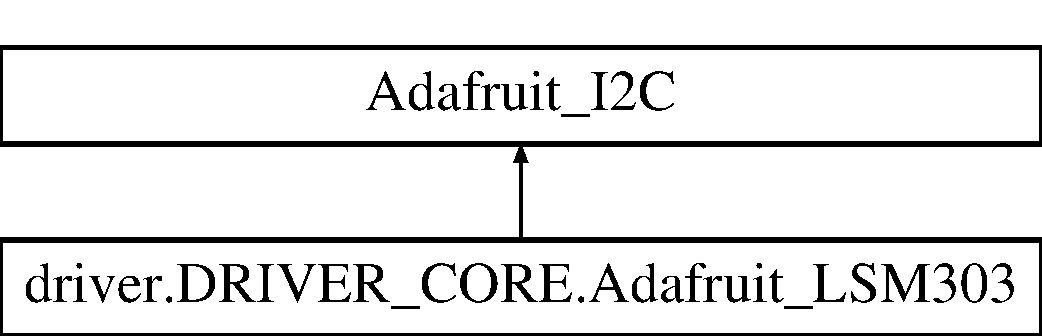
\includegraphics[height=2.000000cm]{classdriver_1_1DRIVER__CORE_1_1Adafruit__LSM303}
\end{center}
\end{figure}
\subsection*{Public Member Functions}
\begin{DoxyCompactItemize}
\item 
\hypertarget{classdriver_1_1DRIVER__CORE_1_1Adafruit__LSM303_ae5cf180d90f8866edaab4807bbe8f7bc}{}def {\bfseries \+\_\+\+\_\+init\+\_\+\+\_\+}\label{classdriver_1_1DRIVER__CORE_1_1Adafruit__LSM303_ae5cf180d90f8866edaab4807bbe8f7bc}

\item 
\hypertarget{classdriver_1_1DRIVER__CORE_1_1Adafruit__LSM303_a73f30f042346b5134d46ac40ea05287c}{}def {\bfseries accel12}\label{classdriver_1_1DRIVER__CORE_1_1Adafruit__LSM303_a73f30f042346b5134d46ac40ea05287c}

\item 
\hypertarget{classdriver_1_1DRIVER__CORE_1_1Adafruit__LSM303_a14da193d80d260f4d95a2636067685ce}{}def {\bfseries mag16}\label{classdriver_1_1DRIVER__CORE_1_1Adafruit__LSM303_a14da193d80d260f4d95a2636067685ce}

\item 
\hypertarget{classdriver_1_1DRIVER__CORE_1_1Adafruit__LSM303_a120ac3815a90e0b4ff49ae60958d568c}{}def {\bfseries read}\label{classdriver_1_1DRIVER__CORE_1_1Adafruit__LSM303_a120ac3815a90e0b4ff49ae60958d568c}

\item 
\hypertarget{classdriver_1_1DRIVER__CORE_1_1Adafruit__LSM303_a91452cc4c7ef0ab07e886843e1cc90dd}{}def {\bfseries set\+Mag\+Gain}\label{classdriver_1_1DRIVER__CORE_1_1Adafruit__LSM303_a91452cc4c7ef0ab07e886843e1cc90dd}

\end{DoxyCompactItemize}
\subsection*{Public Attributes}
\begin{DoxyCompactItemize}
\item 
\hypertarget{classdriver_1_1DRIVER__CORE_1_1Adafruit__LSM303_a17adc9c743af3a5829980b8a702c64d1}{}{\bfseries accel}\label{classdriver_1_1DRIVER__CORE_1_1Adafruit__LSM303_a17adc9c743af3a5829980b8a702c64d1}

\item 
\hypertarget{classdriver_1_1DRIVER__CORE_1_1Adafruit__LSM303_a2afbe1cbd59ce00af91d9e431eb2b391}{}{\bfseries mag}\label{classdriver_1_1DRIVER__CORE_1_1Adafruit__LSM303_a2afbe1cbd59ce00af91d9e431eb2b391}

\end{DoxyCompactItemize}
\subsection*{Static Public Attributes}
\begin{DoxyCompactItemize}
\item 
\hypertarget{classdriver_1_1DRIVER__CORE_1_1Adafruit__LSM303_a24ad319884adc1c09dd29f423b8b6692}{}tuple {\bfseries L\+S\+M303\+\_\+\+A\+D\+D\+R\+E\+S\+S\+\_\+\+A\+C\+C\+E\+L} = (0x32 $>$$>$ 1)\label{classdriver_1_1DRIVER__CORE_1_1Adafruit__LSM303_a24ad319884adc1c09dd29f423b8b6692}

\item 
\hypertarget{classdriver_1_1DRIVER__CORE_1_1Adafruit__LSM303_a0b503ed9efa5d7a4d6edc9e02d1cd61f}{}tuple {\bfseries L\+S\+M303\+\_\+\+A\+D\+D\+R\+E\+S\+S\+\_\+\+M\+A\+G} = (0x3\+C $>$$>$ 1)\label{classdriver_1_1DRIVER__CORE_1_1Adafruit__LSM303_a0b503ed9efa5d7a4d6edc9e02d1cd61f}

\item 
\hypertarget{classdriver_1_1DRIVER__CORE_1_1Adafruit__LSM303_ac907d5dc53fef3f3a59a99e7dd969de2}{}int {\bfseries L\+S\+M303\+\_\+\+R\+E\+G\+I\+S\+T\+E\+R\+\_\+\+A\+C\+C\+E\+L\+\_\+\+C\+T\+R\+L\+\_\+\+R\+E\+G1\+\_\+\+A} = 0x20\label{classdriver_1_1DRIVER__CORE_1_1Adafruit__LSM303_ac907d5dc53fef3f3a59a99e7dd969de2}

\item 
\hypertarget{classdriver_1_1DRIVER__CORE_1_1Adafruit__LSM303_ab9fecee305847de9273f660412fccf01}{}int {\bfseries L\+S\+M303\+\_\+\+R\+E\+G\+I\+S\+T\+E\+R\+\_\+\+A\+C\+C\+E\+L\+\_\+\+C\+T\+R\+L\+\_\+\+R\+E\+G4\+\_\+\+A} = 0x23\label{classdriver_1_1DRIVER__CORE_1_1Adafruit__LSM303_ab9fecee305847de9273f660412fccf01}

\item 
\hypertarget{classdriver_1_1DRIVER__CORE_1_1Adafruit__LSM303_a9db7d714f9448a3ac4121457f1996634}{}int {\bfseries L\+S\+M303\+\_\+\+R\+E\+G\+I\+S\+T\+E\+R\+\_\+\+A\+C\+C\+E\+L\+\_\+\+O\+U\+T\+\_\+\+X\+\_\+\+L\+\_\+\+A} = 0x28\label{classdriver_1_1DRIVER__CORE_1_1Adafruit__LSM303_a9db7d714f9448a3ac4121457f1996634}

\item 
\hypertarget{classdriver_1_1DRIVER__CORE_1_1Adafruit__LSM303_a9ce34b06b2a881fe87f4acf7275e788d}{}int {\bfseries L\+S\+M303\+\_\+\+R\+E\+G\+I\+S\+T\+E\+R\+\_\+\+M\+A\+G\+\_\+\+C\+R\+B\+\_\+\+R\+E\+G\+\_\+\+M} = 0x01\label{classdriver_1_1DRIVER__CORE_1_1Adafruit__LSM303_a9ce34b06b2a881fe87f4acf7275e788d}

\item 
\hypertarget{classdriver_1_1DRIVER__CORE_1_1Adafruit__LSM303_af17a9acb25451a4a2c5f388ff6f95754}{}int {\bfseries L\+S\+M303\+\_\+\+R\+E\+G\+I\+S\+T\+E\+R\+\_\+\+M\+A\+G\+\_\+\+M\+R\+\_\+\+R\+E\+G\+\_\+\+M} = 0x02\label{classdriver_1_1DRIVER__CORE_1_1Adafruit__LSM303_af17a9acb25451a4a2c5f388ff6f95754}

\item 
\hypertarget{classdriver_1_1DRIVER__CORE_1_1Adafruit__LSM303_a39399d95adf47130963ad6228b41f5b5}{}int {\bfseries L\+S\+M303\+\_\+\+R\+E\+G\+I\+S\+T\+E\+R\+\_\+\+M\+A\+G\+\_\+\+O\+U\+T\+\_\+\+X\+\_\+\+H\+\_\+\+M} = 0x03\label{classdriver_1_1DRIVER__CORE_1_1Adafruit__LSM303_a39399d95adf47130963ad6228b41f5b5}

\item 
\hypertarget{classdriver_1_1DRIVER__CORE_1_1Adafruit__LSM303_a7f838baa79a6ae3da80e428f07c0b9ae}{}int {\bfseries L\+S\+M303\+\_\+\+M\+A\+G\+G\+A\+I\+N\+\_\+1\+\_\+3} = 0x20\label{classdriver_1_1DRIVER__CORE_1_1Adafruit__LSM303_a7f838baa79a6ae3da80e428f07c0b9ae}

\item 
\hypertarget{classdriver_1_1DRIVER__CORE_1_1Adafruit__LSM303_a895624eb31381290c41eb4ba15762a21}{}int {\bfseries L\+S\+M303\+\_\+\+M\+A\+G\+G\+A\+I\+N\+\_\+1\+\_\+9} = 0x40\label{classdriver_1_1DRIVER__CORE_1_1Adafruit__LSM303_a895624eb31381290c41eb4ba15762a21}

\item 
\hypertarget{classdriver_1_1DRIVER__CORE_1_1Adafruit__LSM303_a690a2ccf1305ddb8e369e42e140a3d9e}{}int {\bfseries L\+S\+M303\+\_\+\+M\+A\+G\+G\+A\+I\+N\+\_\+2\+\_\+5} = 0x60\label{classdriver_1_1DRIVER__CORE_1_1Adafruit__LSM303_a690a2ccf1305ddb8e369e42e140a3d9e}

\item 
\hypertarget{classdriver_1_1DRIVER__CORE_1_1Adafruit__LSM303_aabf347d0927ecaea47e318cc804e10a0}{}int {\bfseries L\+S\+M303\+\_\+\+M\+A\+G\+G\+A\+I\+N\+\_\+4\+\_\+0} = 0x80\label{classdriver_1_1DRIVER__CORE_1_1Adafruit__LSM303_aabf347d0927ecaea47e318cc804e10a0}

\item 
\hypertarget{classdriver_1_1DRIVER__CORE_1_1Adafruit__LSM303_a1875f919180b6da6408c2d005bb8bdad}{}int {\bfseries L\+S\+M303\+\_\+\+M\+A\+G\+G\+A\+I\+N\+\_\+4\+\_\+7} = 0x\+A0\label{classdriver_1_1DRIVER__CORE_1_1Adafruit__LSM303_a1875f919180b6da6408c2d005bb8bdad}

\item 
\hypertarget{classdriver_1_1DRIVER__CORE_1_1Adafruit__LSM303_a9dfa52c66b43d044d18e642243a4c15d}{}int {\bfseries L\+S\+M303\+\_\+\+M\+A\+G\+G\+A\+I\+N\+\_\+5\+\_\+6} = 0x\+C0\label{classdriver_1_1DRIVER__CORE_1_1Adafruit__LSM303_a9dfa52c66b43d044d18e642243a4c15d}

\item 
\hypertarget{classdriver_1_1DRIVER__CORE_1_1Adafruit__LSM303_a4c33c59d6577266becd976da47b46e7c}{}int {\bfseries L\+S\+M303\+\_\+\+M\+A\+G\+G\+A\+I\+N\+\_\+8\+\_\+1} = 0x\+E0\label{classdriver_1_1DRIVER__CORE_1_1Adafruit__LSM303_a4c33c59d6577266becd976da47b46e7c}

\end{DoxyCompactItemize}


\subsection{Detailed Description}
\begin{DoxyVerb}Python library for Adafruit Flora Accelerometer/Compass Sensor (LSM303).
This is pretty much a direct port of the current Arduino library and is
similarly incomplete (e.g. no orientation value returned from read()
method).  This does add optional high resolution mode to accelerometer
though.

Copyright 2013 Adafruit Industries

Version 0.1

Revised October 10, 2014

Revision Author: Isaac DeSouza (IDS LABS)

Copyright 2014 IDS LABS
\end{DoxyVerb}
 

The documentation for this class was generated from the following file\+:\begin{DoxyCompactItemize}
\item 
D\+R\+I\+V\+E\+R\+\_\+\+C\+O\+R\+E.\+py\end{DoxyCompactItemize}

\hypertarget{classdriver_1_1LOGITECH__GAMEPAD__DRIVER_1_1LogitechGamepadDriver_1_1GamepadThread}{}\section{driver.\+L\+O\+G\+I\+T\+E\+C\+H\+\_\+\+G\+A\+M\+E\+P\+A\+D\+\_\+\+D\+R\+I\+V\+E\+R.\+Logitech\+Gamepad\+Driver.\+Gamepad\+Thread Class Reference}
\label{classdriver_1_1LOGITECH__GAMEPAD__DRIVER_1_1LogitechGamepadDriver_1_1GamepadThread}\index{driver.\+L\+O\+G\+I\+T\+E\+C\+H\+\_\+\+G\+A\+M\+E\+P\+A\+D\+\_\+\+D\+R\+I\+V\+E\+R.\+Logitech\+Gamepad\+Driver.\+Gamepad\+Thread@{driver.\+L\+O\+G\+I\+T\+E\+C\+H\+\_\+\+G\+A\+M\+E\+P\+A\+D\+\_\+\+D\+R\+I\+V\+E\+R.\+Logitech\+Gamepad\+Driver.\+Gamepad\+Thread}}
Inheritance diagram for driver.\+L\+O\+G\+I\+T\+E\+C\+H\+\_\+\+G\+A\+M\+E\+P\+A\+D\+\_\+\+D\+R\+I\+V\+E\+R.\+Logitech\+Gamepad\+Driver.\+Gamepad\+Thread\+:\begin{figure}[H]
\begin{center}
\leavevmode
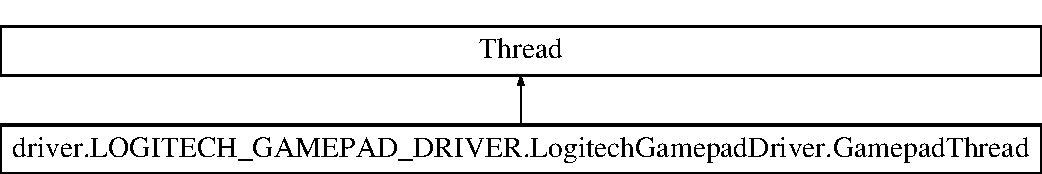
\includegraphics[height=1.166667cm]{classdriver_1_1LOGITECH__GAMEPAD__DRIVER_1_1LogitechGamepadDriver_1_1GamepadThread}
\end{center}
\end{figure}
\subsection*{Public Member Functions}
\begin{DoxyCompactItemize}
\item 
def \hyperlink{classdriver_1_1LOGITECH__GAMEPAD__DRIVER_1_1LogitechGamepadDriver_1_1GamepadThread_aa08ed3fd5770b7518dd3c3672adb37d3}{\+\_\+\+\_\+init\+\_\+\+\_\+}
\item 
def \hyperlink{classdriver_1_1LOGITECH__GAMEPAD__DRIVER_1_1LogitechGamepadDriver_1_1GamepadThread_a1081a12fcf001359ba0755676ef9db77}{run}
\item 
def \hyperlink{classdriver_1_1LOGITECH__GAMEPAD__DRIVER_1_1LogitechGamepadDriver_1_1GamepadThread_aa08ed3fd5770b7518dd3c3672adb37d3}{\+\_\+\+\_\+init\+\_\+\+\_\+}
\item 
def \hyperlink{classdriver_1_1LOGITECH__GAMEPAD__DRIVER_1_1LogitechGamepadDriver_1_1GamepadThread_a1081a12fcf001359ba0755676ef9db77}{run}
\end{DoxyCompactItemize}
\subsection*{Public Attributes}
\begin{DoxyCompactItemize}
\item 
\hyperlink{classdriver_1_1LOGITECH__GAMEPAD__DRIVER_1_1LogitechGamepadDriver_1_1GamepadThread_abede3a32608fc0d308e1cebcbd507eef}{parent}
\item 
\hyperlink{classdriver_1_1LOGITECH__GAMEPAD__DRIVER_1_1LogitechGamepadDriver_1_1GamepadThread_a01174be3f4261cd2dc0510a95907ae24}{num}
\item 
\hyperlink{classdriver_1_1LOGITECH__GAMEPAD__DRIVER_1_1LogitechGamepadDriver_1_1GamepadThread_a013099b962d25f2d0b6ed991527ba55b}{do\+Stuff}
\item 
\hyperlink{classdriver_1_1LOGITECH__GAMEPAD__DRIVER_1_1LogitechGamepadDriver_1_1GamepadThread_aefd0103bf5744b989ad40c8545f35388}{delay}
\end{DoxyCompactItemize}


\subsection{Constructor \& Destructor Documentation}
\hypertarget{classdriver_1_1LOGITECH__GAMEPAD__DRIVER_1_1LogitechGamepadDriver_1_1GamepadThread_aa08ed3fd5770b7518dd3c3672adb37d3}{}\index{driver\+::\+L\+O\+G\+I\+T\+E\+C\+H\+\_\+\+G\+A\+M\+E\+P\+A\+D\+\_\+\+D\+R\+I\+V\+E\+R\+::\+Logitech\+Gamepad\+Driver\+::\+Gamepad\+Thread@{driver\+::\+L\+O\+G\+I\+T\+E\+C\+H\+\_\+\+G\+A\+M\+E\+P\+A\+D\+\_\+\+D\+R\+I\+V\+E\+R\+::\+Logitech\+Gamepad\+Driver\+::\+Gamepad\+Thread}!\+\_\+\+\_\+init\+\_\+\+\_\+@{\+\_\+\+\_\+init\+\_\+\+\_\+}}
\index{\+\_\+\+\_\+init\+\_\+\+\_\+@{\+\_\+\+\_\+init\+\_\+\+\_\+}!driver\+::\+L\+O\+G\+I\+T\+E\+C\+H\+\_\+\+G\+A\+M\+E\+P\+A\+D\+\_\+\+D\+R\+I\+V\+E\+R\+::\+Logitech\+Gamepad\+Driver\+::\+Gamepad\+Thread@{driver\+::\+L\+O\+G\+I\+T\+E\+C\+H\+\_\+\+G\+A\+M\+E\+P\+A\+D\+\_\+\+D\+R\+I\+V\+E\+R\+::\+Logitech\+Gamepad\+Driver\+::\+Gamepad\+Thread}}
\subsubsection[{\+\_\+\+\_\+init\+\_\+\+\_\+}]{\setlength{\rightskip}{0pt plus 5cm}def driver.\+L\+O\+G\+I\+T\+E\+C\+H\+\_\+\+G\+A\+M\+E\+P\+A\+D\+\_\+\+D\+R\+I\+V\+E\+R.\+Logitech\+Gamepad\+Driver.\+Gamepad\+Thread.\+\_\+\+\_\+init\+\_\+\+\_\+ (
\begin{DoxyParamCaption}
\item[{}]{self, }
\item[{}]{parent, }
\item[{}]{num, }
\item[{}]{do\+Stuff, }
\item[{}]{delay}
\end{DoxyParamCaption}
)}\label{classdriver_1_1LOGITECH__GAMEPAD__DRIVER_1_1LogitechGamepadDriver_1_1GamepadThread_aa08ed3fd5770b7518dd3c3672adb37d3}
\hypertarget{classdriver_1_1LOGITECH__GAMEPAD__DRIVER_1_1LogitechGamepadDriver_1_1GamepadThread_aa08ed3fd5770b7518dd3c3672adb37d3}{}\index{driver\+::\+L\+O\+G\+I\+T\+E\+C\+H\+\_\+\+G\+A\+M\+E\+P\+A\+D\+\_\+\+D\+R\+I\+V\+E\+R\+::\+Logitech\+Gamepad\+Driver\+::\+Gamepad\+Thread@{driver\+::\+L\+O\+G\+I\+T\+E\+C\+H\+\_\+\+G\+A\+M\+E\+P\+A\+D\+\_\+\+D\+R\+I\+V\+E\+R\+::\+Logitech\+Gamepad\+Driver\+::\+Gamepad\+Thread}!\+\_\+\+\_\+init\+\_\+\+\_\+@{\+\_\+\+\_\+init\+\_\+\+\_\+}}
\index{\+\_\+\+\_\+init\+\_\+\+\_\+@{\+\_\+\+\_\+init\+\_\+\+\_\+}!driver\+::\+L\+O\+G\+I\+T\+E\+C\+H\+\_\+\+G\+A\+M\+E\+P\+A\+D\+\_\+\+D\+R\+I\+V\+E\+R\+::\+Logitech\+Gamepad\+Driver\+::\+Gamepad\+Thread@{driver\+::\+L\+O\+G\+I\+T\+E\+C\+H\+\_\+\+G\+A\+M\+E\+P\+A\+D\+\_\+\+D\+R\+I\+V\+E\+R\+::\+Logitech\+Gamepad\+Driver\+::\+Gamepad\+Thread}}
\subsubsection[{\+\_\+\+\_\+init\+\_\+\+\_\+}]{\setlength{\rightskip}{0pt plus 5cm}def driver.\+L\+O\+G\+I\+T\+E\+C\+H\+\_\+\+G\+A\+M\+E\+P\+A\+D\+\_\+\+D\+R\+I\+V\+E\+R.\+Logitech\+Gamepad\+Driver.\+Gamepad\+Thread.\+\_\+\+\_\+init\+\_\+\+\_\+ (
\begin{DoxyParamCaption}
\item[{}]{self, }
\item[{}]{parent, }
\item[{}]{num, }
\item[{}]{do\+Stuff, }
\item[{}]{delay}
\end{DoxyParamCaption}
)}\label{classdriver_1_1LOGITECH__GAMEPAD__DRIVER_1_1LogitechGamepadDriver_1_1GamepadThread_aa08ed3fd5770b7518dd3c3672adb37d3}


\subsection{Member Function Documentation}
\hypertarget{classdriver_1_1LOGITECH__GAMEPAD__DRIVER_1_1LogitechGamepadDriver_1_1GamepadThread_a1081a12fcf001359ba0755676ef9db77}{}\index{driver\+::\+L\+O\+G\+I\+T\+E\+C\+H\+\_\+\+G\+A\+M\+E\+P\+A\+D\+\_\+\+D\+R\+I\+V\+E\+R\+::\+Logitech\+Gamepad\+Driver\+::\+Gamepad\+Thread@{driver\+::\+L\+O\+G\+I\+T\+E\+C\+H\+\_\+\+G\+A\+M\+E\+P\+A\+D\+\_\+\+D\+R\+I\+V\+E\+R\+::\+Logitech\+Gamepad\+Driver\+::\+Gamepad\+Thread}!run@{run}}
\index{run@{run}!driver\+::\+L\+O\+G\+I\+T\+E\+C\+H\+\_\+\+G\+A\+M\+E\+P\+A\+D\+\_\+\+D\+R\+I\+V\+E\+R\+::\+Logitech\+Gamepad\+Driver\+::\+Gamepad\+Thread@{driver\+::\+L\+O\+G\+I\+T\+E\+C\+H\+\_\+\+G\+A\+M\+E\+P\+A\+D\+\_\+\+D\+R\+I\+V\+E\+R\+::\+Logitech\+Gamepad\+Driver\+::\+Gamepad\+Thread}}
\subsubsection[{run}]{\setlength{\rightskip}{0pt plus 5cm}def driver.\+L\+O\+G\+I\+T\+E\+C\+H\+\_\+\+G\+A\+M\+E\+P\+A\+D\+\_\+\+D\+R\+I\+V\+E\+R.\+Logitech\+Gamepad\+Driver.\+Gamepad\+Thread.\+run (
\begin{DoxyParamCaption}
\item[{}]{self}
\end{DoxyParamCaption}
)}\label{classdriver_1_1LOGITECH__GAMEPAD__DRIVER_1_1LogitechGamepadDriver_1_1GamepadThread_a1081a12fcf001359ba0755676ef9db77}
\hypertarget{classdriver_1_1LOGITECH__GAMEPAD__DRIVER_1_1LogitechGamepadDriver_1_1GamepadThread_a1081a12fcf001359ba0755676ef9db77}{}\index{driver\+::\+L\+O\+G\+I\+T\+E\+C\+H\+\_\+\+G\+A\+M\+E\+P\+A\+D\+\_\+\+D\+R\+I\+V\+E\+R\+::\+Logitech\+Gamepad\+Driver\+::\+Gamepad\+Thread@{driver\+::\+L\+O\+G\+I\+T\+E\+C\+H\+\_\+\+G\+A\+M\+E\+P\+A\+D\+\_\+\+D\+R\+I\+V\+E\+R\+::\+Logitech\+Gamepad\+Driver\+::\+Gamepad\+Thread}!run@{run}}
\index{run@{run}!driver\+::\+L\+O\+G\+I\+T\+E\+C\+H\+\_\+\+G\+A\+M\+E\+P\+A\+D\+\_\+\+D\+R\+I\+V\+E\+R\+::\+Logitech\+Gamepad\+Driver\+::\+Gamepad\+Thread@{driver\+::\+L\+O\+G\+I\+T\+E\+C\+H\+\_\+\+G\+A\+M\+E\+P\+A\+D\+\_\+\+D\+R\+I\+V\+E\+R\+::\+Logitech\+Gamepad\+Driver\+::\+Gamepad\+Thread}}
\subsubsection[{run}]{\setlength{\rightskip}{0pt plus 5cm}def driver.\+L\+O\+G\+I\+T\+E\+C\+H\+\_\+\+G\+A\+M\+E\+P\+A\+D\+\_\+\+D\+R\+I\+V\+E\+R.\+Logitech\+Gamepad\+Driver.\+Gamepad\+Thread.\+run (
\begin{DoxyParamCaption}
\item[{}]{self}
\end{DoxyParamCaption}
)}\label{classdriver_1_1LOGITECH__GAMEPAD__DRIVER_1_1LogitechGamepadDriver_1_1GamepadThread_a1081a12fcf001359ba0755676ef9db77}


\subsection{Member Data Documentation}
\hypertarget{classdriver_1_1LOGITECH__GAMEPAD__DRIVER_1_1LogitechGamepadDriver_1_1GamepadThread_aefd0103bf5744b989ad40c8545f35388}{}\index{driver\+::\+L\+O\+G\+I\+T\+E\+C\+H\+\_\+\+G\+A\+M\+E\+P\+A\+D\+\_\+\+D\+R\+I\+V\+E\+R\+::\+Logitech\+Gamepad\+Driver\+::\+Gamepad\+Thread@{driver\+::\+L\+O\+G\+I\+T\+E\+C\+H\+\_\+\+G\+A\+M\+E\+P\+A\+D\+\_\+\+D\+R\+I\+V\+E\+R\+::\+Logitech\+Gamepad\+Driver\+::\+Gamepad\+Thread}!delay@{delay}}
\index{delay@{delay}!driver\+::\+L\+O\+G\+I\+T\+E\+C\+H\+\_\+\+G\+A\+M\+E\+P\+A\+D\+\_\+\+D\+R\+I\+V\+E\+R\+::\+Logitech\+Gamepad\+Driver\+::\+Gamepad\+Thread@{driver\+::\+L\+O\+G\+I\+T\+E\+C\+H\+\_\+\+G\+A\+M\+E\+P\+A\+D\+\_\+\+D\+R\+I\+V\+E\+R\+::\+Logitech\+Gamepad\+Driver\+::\+Gamepad\+Thread}}
\subsubsection[{delay}]{\setlength{\rightskip}{0pt plus 5cm}driver.\+L\+O\+G\+I\+T\+E\+C\+H\+\_\+\+G\+A\+M\+E\+P\+A\+D\+\_\+\+D\+R\+I\+V\+E\+R.\+Logitech\+Gamepad\+Driver.\+Gamepad\+Thread.\+delay}\label{classdriver_1_1LOGITECH__GAMEPAD__DRIVER_1_1LogitechGamepadDriver_1_1GamepadThread_aefd0103bf5744b989ad40c8545f35388}
\hypertarget{classdriver_1_1LOGITECH__GAMEPAD__DRIVER_1_1LogitechGamepadDriver_1_1GamepadThread_a013099b962d25f2d0b6ed991527ba55b}{}\index{driver\+::\+L\+O\+G\+I\+T\+E\+C\+H\+\_\+\+G\+A\+M\+E\+P\+A\+D\+\_\+\+D\+R\+I\+V\+E\+R\+::\+Logitech\+Gamepad\+Driver\+::\+Gamepad\+Thread@{driver\+::\+L\+O\+G\+I\+T\+E\+C\+H\+\_\+\+G\+A\+M\+E\+P\+A\+D\+\_\+\+D\+R\+I\+V\+E\+R\+::\+Logitech\+Gamepad\+Driver\+::\+Gamepad\+Thread}!do\+Stuff@{do\+Stuff}}
\index{do\+Stuff@{do\+Stuff}!driver\+::\+L\+O\+G\+I\+T\+E\+C\+H\+\_\+\+G\+A\+M\+E\+P\+A\+D\+\_\+\+D\+R\+I\+V\+E\+R\+::\+Logitech\+Gamepad\+Driver\+::\+Gamepad\+Thread@{driver\+::\+L\+O\+G\+I\+T\+E\+C\+H\+\_\+\+G\+A\+M\+E\+P\+A\+D\+\_\+\+D\+R\+I\+V\+E\+R\+::\+Logitech\+Gamepad\+Driver\+::\+Gamepad\+Thread}}
\subsubsection[{do\+Stuff}]{\setlength{\rightskip}{0pt plus 5cm}driver.\+L\+O\+G\+I\+T\+E\+C\+H\+\_\+\+G\+A\+M\+E\+P\+A\+D\+\_\+\+D\+R\+I\+V\+E\+R.\+Logitech\+Gamepad\+Driver.\+Gamepad\+Thread.\+do\+Stuff}\label{classdriver_1_1LOGITECH__GAMEPAD__DRIVER_1_1LogitechGamepadDriver_1_1GamepadThread_a013099b962d25f2d0b6ed991527ba55b}
\hypertarget{classdriver_1_1LOGITECH__GAMEPAD__DRIVER_1_1LogitechGamepadDriver_1_1GamepadThread_a01174be3f4261cd2dc0510a95907ae24}{}\index{driver\+::\+L\+O\+G\+I\+T\+E\+C\+H\+\_\+\+G\+A\+M\+E\+P\+A\+D\+\_\+\+D\+R\+I\+V\+E\+R\+::\+Logitech\+Gamepad\+Driver\+::\+Gamepad\+Thread@{driver\+::\+L\+O\+G\+I\+T\+E\+C\+H\+\_\+\+G\+A\+M\+E\+P\+A\+D\+\_\+\+D\+R\+I\+V\+E\+R\+::\+Logitech\+Gamepad\+Driver\+::\+Gamepad\+Thread}!num@{num}}
\index{num@{num}!driver\+::\+L\+O\+G\+I\+T\+E\+C\+H\+\_\+\+G\+A\+M\+E\+P\+A\+D\+\_\+\+D\+R\+I\+V\+E\+R\+::\+Logitech\+Gamepad\+Driver\+::\+Gamepad\+Thread@{driver\+::\+L\+O\+G\+I\+T\+E\+C\+H\+\_\+\+G\+A\+M\+E\+P\+A\+D\+\_\+\+D\+R\+I\+V\+E\+R\+::\+Logitech\+Gamepad\+Driver\+::\+Gamepad\+Thread}}
\subsubsection[{num}]{\setlength{\rightskip}{0pt plus 5cm}driver.\+L\+O\+G\+I\+T\+E\+C\+H\+\_\+\+G\+A\+M\+E\+P\+A\+D\+\_\+\+D\+R\+I\+V\+E\+R.\+Logitech\+Gamepad\+Driver.\+Gamepad\+Thread.\+num}\label{classdriver_1_1LOGITECH__GAMEPAD__DRIVER_1_1LogitechGamepadDriver_1_1GamepadThread_a01174be3f4261cd2dc0510a95907ae24}
\hypertarget{classdriver_1_1LOGITECH__GAMEPAD__DRIVER_1_1LogitechGamepadDriver_1_1GamepadThread_abede3a32608fc0d308e1cebcbd507eef}{}\index{driver\+::\+L\+O\+G\+I\+T\+E\+C\+H\+\_\+\+G\+A\+M\+E\+P\+A\+D\+\_\+\+D\+R\+I\+V\+E\+R\+::\+Logitech\+Gamepad\+Driver\+::\+Gamepad\+Thread@{driver\+::\+L\+O\+G\+I\+T\+E\+C\+H\+\_\+\+G\+A\+M\+E\+P\+A\+D\+\_\+\+D\+R\+I\+V\+E\+R\+::\+Logitech\+Gamepad\+Driver\+::\+Gamepad\+Thread}!parent@{parent}}
\index{parent@{parent}!driver\+::\+L\+O\+G\+I\+T\+E\+C\+H\+\_\+\+G\+A\+M\+E\+P\+A\+D\+\_\+\+D\+R\+I\+V\+E\+R\+::\+Logitech\+Gamepad\+Driver\+::\+Gamepad\+Thread@{driver\+::\+L\+O\+G\+I\+T\+E\+C\+H\+\_\+\+G\+A\+M\+E\+P\+A\+D\+\_\+\+D\+R\+I\+V\+E\+R\+::\+Logitech\+Gamepad\+Driver\+::\+Gamepad\+Thread}}
\subsubsection[{parent}]{\setlength{\rightskip}{0pt plus 5cm}driver.\+L\+O\+G\+I\+T\+E\+C\+H\+\_\+\+G\+A\+M\+E\+P\+A\+D\+\_\+\+D\+R\+I\+V\+E\+R.\+Logitech\+Gamepad\+Driver.\+Gamepad\+Thread.\+parent}\label{classdriver_1_1LOGITECH__GAMEPAD__DRIVER_1_1LogitechGamepadDriver_1_1GamepadThread_abede3a32608fc0d308e1cebcbd507eef}


The documentation for this class was generated from the following file\+:\begin{DoxyCompactItemize}
\item 
build/lib.\+linux-\/x86\+\_\+64-\/2.\+7/driver/\hyperlink{build_2lib_8linux-x86__64-2_87_2driver_2LOGITECH__GAMEPAD__DRIVER_8py}{L\+O\+G\+I\+T\+E\+C\+H\+\_\+\+G\+A\+M\+E\+P\+A\+D\+\_\+\+D\+R\+I\+V\+E\+R.\+py}\end{DoxyCompactItemize}

\hypertarget{classdriver_1_1i2c__lib_1_1i2c__device}{}\section{driver.\+i2c\+\_\+lib.\+i2c\+\_\+device Class Reference}
\label{classdriver_1_1i2c__lib_1_1i2c__device}\index{driver.\+i2c\+\_\+lib.\+i2c\+\_\+device@{driver.\+i2c\+\_\+lib.\+i2c\+\_\+device}}
\subsection*{Public Member Functions}
\begin{DoxyCompactItemize}
\item 
\hypertarget{classdriver_1_1i2c__lib_1_1i2c__device_a6f4de0589e9fc9d80dfcbe78764adca6}{}def {\bfseries \+\_\+\+\_\+init\+\_\+\+\_\+}\label{classdriver_1_1i2c__lib_1_1i2c__device_a6f4de0589e9fc9d80dfcbe78764adca6}

\item 
\hypertarget{classdriver_1_1i2c__lib_1_1i2c__device_a4793439f363c2b22a7f3beae6074f755}{}def {\bfseries write\+\_\+cmd}\label{classdriver_1_1i2c__lib_1_1i2c__device_a4793439f363c2b22a7f3beae6074f755}

\item 
\hypertarget{classdriver_1_1i2c__lib_1_1i2c__device_ae998e6b6651a038c5b5466ae941e0eb8}{}def {\bfseries write\+\_\+cmd\+\_\+arg}\label{classdriver_1_1i2c__lib_1_1i2c__device_ae998e6b6651a038c5b5466ae941e0eb8}

\item 
\hypertarget{classdriver_1_1i2c__lib_1_1i2c__device_ae270018219f2f96ec9e37e36065d2edc}{}def {\bfseries write\+\_\+block\+\_\+data}\label{classdriver_1_1i2c__lib_1_1i2c__device_ae270018219f2f96ec9e37e36065d2edc}

\item 
\hypertarget{classdriver_1_1i2c__lib_1_1i2c__device_a9a8d9b4cc3d3890baa0738c9fa60ef4b}{}def {\bfseries read}\label{classdriver_1_1i2c__lib_1_1i2c__device_a9a8d9b4cc3d3890baa0738c9fa60ef4b}

\item 
\hypertarget{classdriver_1_1i2c__lib_1_1i2c__device_a7960797223c6a315d764f8b1ff11a8f2}{}def {\bfseries read\+\_\+data}\label{classdriver_1_1i2c__lib_1_1i2c__device_a7960797223c6a315d764f8b1ff11a8f2}

\item 
\hypertarget{classdriver_1_1i2c__lib_1_1i2c__device_ad837253a1137bd4ae725f80640ace947}{}def {\bfseries read\+\_\+block\+\_\+data}\label{classdriver_1_1i2c__lib_1_1i2c__device_ad837253a1137bd4ae725f80640ace947}

\end{DoxyCompactItemize}
\subsection*{Public Attributes}
\begin{DoxyCompactItemize}
\item 
\hypertarget{classdriver_1_1i2c__lib_1_1i2c__device_a9cfbff86867d526e3bcb5213d80b6f2c}{}{\bfseries addr}\label{classdriver_1_1i2c__lib_1_1i2c__device_a9cfbff86867d526e3bcb5213d80b6f2c}

\item 
\hypertarget{classdriver_1_1i2c__lib_1_1i2c__device_ac57614bbc2affcaf48f890e8a79c1e96}{}{\bfseries bus}\label{classdriver_1_1i2c__lib_1_1i2c__device_ac57614bbc2affcaf48f890e8a79c1e96}

\end{DoxyCompactItemize}


The documentation for this class was generated from the following file\+:\begin{DoxyCompactItemize}
\item 
i2c\+\_\+lib.\+py\end{DoxyCompactItemize}

\hypertarget{classdriver_1_1LCD__DRIVER_1_1LCD}{}\section{driver.\+L\+C\+D\+\_\+\+D\+R\+I\+V\+E\+R.\+L\+C\+D Class Reference}
\label{classdriver_1_1LCD__DRIVER_1_1LCD}\index{driver.\+L\+C\+D\+\_\+\+D\+R\+I\+V\+E\+R.\+L\+C\+D@{driver.\+L\+C\+D\+\_\+\+D\+R\+I\+V\+E\+R.\+L\+C\+D}}
\subsection*{Public Member Functions}
\begin{DoxyCompactItemize}
\item 
\hypertarget{classdriver_1_1LCD__DRIVER_1_1LCD_a20225b4d0a79ea608ab2788528735b17}{}def {\bfseries \+\_\+\+\_\+init\+\_\+\+\_\+}\label{classdriver_1_1LCD__DRIVER_1_1LCD_a20225b4d0a79ea608ab2788528735b17}

\item 
\hypertarget{classdriver_1_1LCD__DRIVER_1_1LCD_a15e214b2ce2f4e8e6e4eb46db360eb17}{}def {\bfseries lcd\+\_\+strobe}\label{classdriver_1_1LCD__DRIVER_1_1LCD_a15e214b2ce2f4e8e6e4eb46db360eb17}

\item 
\hypertarget{classdriver_1_1LCD__DRIVER_1_1LCD_ac5e728a550c74f93db7aeac717f71f56}{}def {\bfseries lcd\+\_\+backlight}\label{classdriver_1_1LCD__DRIVER_1_1LCD_ac5e728a550c74f93db7aeac717f71f56}

\item 
\hypertarget{classdriver_1_1LCD__DRIVER_1_1LCD_a50b4cd9441fc0869a3fc02823e1c4b50}{}def {\bfseries lcd\+\_\+write\+\_\+four\+\_\+bits}\label{classdriver_1_1LCD__DRIVER_1_1LCD_a50b4cd9441fc0869a3fc02823e1c4b50}

\item 
\hypertarget{classdriver_1_1LCD__DRIVER_1_1LCD_ad163c5a30bf46c9b7e794af4c5ee1580}{}def {\bfseries write}\label{classdriver_1_1LCD__DRIVER_1_1LCD_ad163c5a30bf46c9b7e794af4c5ee1580}

\item 
\hypertarget{classdriver_1_1LCD__DRIVER_1_1LCD_a234077a291a2a5fca1bac4e9cf6c05d0}{}def {\bfseries lcd\+\_\+display\+\_\+string}\label{classdriver_1_1LCD__DRIVER_1_1LCD_a234077a291a2a5fca1bac4e9cf6c05d0}

\item 
\hypertarget{classdriver_1_1LCD__DRIVER_1_1LCD_a6d9ced9d16566a567806e0bc2db053b4}{}def {\bfseries lcd\+\_\+clear}\label{classdriver_1_1LCD__DRIVER_1_1LCD_a6d9ced9d16566a567806e0bc2db053b4}

\item 
\hypertarget{classdriver_1_1LCD__DRIVER_1_1LCD_a4b8df3a45944a01d6a12b88f79d0d337}{}def {\bfseries write\+\_\+line}\label{classdriver_1_1LCD__DRIVER_1_1LCD_a4b8df3a45944a01d6a12b88f79d0d337}

\end{DoxyCompactItemize}
\subsection*{Public Attributes}
\begin{DoxyCompactItemize}
\item 
\hypertarget{classdriver_1_1LCD__DRIVER_1_1LCD_ac0009701948020eab39981e6db4f8b7e}{}{\bfseries lcd\+\_\+device}\label{classdriver_1_1LCD__DRIVER_1_1LCD_ac0009701948020eab39981e6db4f8b7e}

\end{DoxyCompactItemize}
\subsection*{Static Public Attributes}
\begin{DoxyCompactItemize}
\item 
\hypertarget{classdriver_1_1LCD__DRIVER_1_1LCD_a0061f642609eb37b58a8df87246def6d}{}int {\bfseries A\+D\+D\+R\+E\+S\+S} = 0x27\label{classdriver_1_1LCD__DRIVER_1_1LCD_a0061f642609eb37b58a8df87246def6d}

\item 
\hypertarget{classdriver_1_1LCD__DRIVER_1_1LCD_a299a1b5139186147d2365fc3a428c840}{}int {\bfseries L\+C\+D\+\_\+\+C\+L\+E\+A\+R\+D\+I\+S\+P\+L\+A\+Y} = 0x01\label{classdriver_1_1LCD__DRIVER_1_1LCD_a299a1b5139186147d2365fc3a428c840}

\item 
\hypertarget{classdriver_1_1LCD__DRIVER_1_1LCD_ab1c8daf615550583049053593bff7c34}{}int {\bfseries L\+C\+D\+\_\+\+R\+E\+T\+U\+R\+N\+H\+O\+M\+E} = 0x02\label{classdriver_1_1LCD__DRIVER_1_1LCD_ab1c8daf615550583049053593bff7c34}

\item 
\hypertarget{classdriver_1_1LCD__DRIVER_1_1LCD_aa8e41e4b48292db9fcc0bd02f670499b}{}int {\bfseries L\+C\+D\+\_\+\+E\+N\+T\+R\+Y\+M\+O\+D\+E\+S\+E\+T} = 0x04\label{classdriver_1_1LCD__DRIVER_1_1LCD_aa8e41e4b48292db9fcc0bd02f670499b}

\item 
\hypertarget{classdriver_1_1LCD__DRIVER_1_1LCD_a3409648ce4331caf45832bf19bc7984b}{}int {\bfseries L\+C\+D\+\_\+\+D\+I\+S\+P\+L\+A\+Y\+C\+O\+N\+T\+R\+O\+L} = 0x08\label{classdriver_1_1LCD__DRIVER_1_1LCD_a3409648ce4331caf45832bf19bc7984b}

\item 
\hypertarget{classdriver_1_1LCD__DRIVER_1_1LCD_a6e47d1add960ea5b04024403d9d25e04}{}int {\bfseries L\+C\+D\+\_\+\+C\+U\+R\+S\+O\+R\+S\+H\+I\+F\+T} = 0x10\label{classdriver_1_1LCD__DRIVER_1_1LCD_a6e47d1add960ea5b04024403d9d25e04}

\item 
\hypertarget{classdriver_1_1LCD__DRIVER_1_1LCD_adfe7a7294af65f234ecc08c47a59e9be}{}int {\bfseries L\+C\+D\+\_\+\+F\+U\+N\+C\+T\+I\+O\+N\+S\+E\+T} = 0x20\label{classdriver_1_1LCD__DRIVER_1_1LCD_adfe7a7294af65f234ecc08c47a59e9be}

\item 
\hypertarget{classdriver_1_1LCD__DRIVER_1_1LCD_a7e912765df7dedabcb7dd02d8c07b1dc}{}int {\bfseries L\+C\+D\+\_\+\+S\+E\+T\+C\+G\+R\+A\+M\+A\+D\+D\+R} = 0x40\label{classdriver_1_1LCD__DRIVER_1_1LCD_a7e912765df7dedabcb7dd02d8c07b1dc}

\item 
\hypertarget{classdriver_1_1LCD__DRIVER_1_1LCD_a921474b833fcba1fe8d9d50fa2055776}{}int {\bfseries L\+C\+D\+\_\+\+S\+E\+T\+D\+D\+R\+A\+M\+A\+D\+D\+R} = 0x80\label{classdriver_1_1LCD__DRIVER_1_1LCD_a921474b833fcba1fe8d9d50fa2055776}

\item 
\hypertarget{classdriver_1_1LCD__DRIVER_1_1LCD_a6bc7920d4f35acb30387f1af2ad0994d}{}int {\bfseries L\+C\+D\+\_\+\+E\+N\+T\+R\+Y\+R\+I\+G\+H\+T} = 0x00\label{classdriver_1_1LCD__DRIVER_1_1LCD_a6bc7920d4f35acb30387f1af2ad0994d}

\item 
\hypertarget{classdriver_1_1LCD__DRIVER_1_1LCD_a29a167818e530e0b99be3a84450bdb91}{}int {\bfseries L\+C\+D\+\_\+\+E\+N\+T\+R\+Y\+L\+E\+F\+T} = 0x02\label{classdriver_1_1LCD__DRIVER_1_1LCD_a29a167818e530e0b99be3a84450bdb91}

\item 
\hypertarget{classdriver_1_1LCD__DRIVER_1_1LCD_a37c462f71833cb0ce4c36849277d1c43}{}int {\bfseries L\+C\+D\+\_\+\+E\+N\+T\+R\+Y\+S\+H\+I\+F\+T\+I\+N\+C\+R\+E\+M\+E\+N\+T} = 0x01\label{classdriver_1_1LCD__DRIVER_1_1LCD_a37c462f71833cb0ce4c36849277d1c43}

\item 
\hypertarget{classdriver_1_1LCD__DRIVER_1_1LCD_a1eb9d5c133147cdc54f923d954375ea1}{}int {\bfseries L\+C\+D\+\_\+\+E\+N\+T\+R\+Y\+S\+H\+I\+F\+T\+D\+E\+C\+R\+E\+M\+E\+N\+T} = 0x00\label{classdriver_1_1LCD__DRIVER_1_1LCD_a1eb9d5c133147cdc54f923d954375ea1}

\item 
\hypertarget{classdriver_1_1LCD__DRIVER_1_1LCD_aaed9b4664cf1eb0523304b2047e8884c}{}int {\bfseries L\+C\+D\+\_\+\+D\+I\+S\+P\+L\+A\+Y\+O\+N} = 0x04\label{classdriver_1_1LCD__DRIVER_1_1LCD_aaed9b4664cf1eb0523304b2047e8884c}

\item 
\hypertarget{classdriver_1_1LCD__DRIVER_1_1LCD_add6574491ae0ed518608872bec12cfa8}{}int {\bfseries L\+C\+D\+\_\+\+D\+I\+S\+P\+L\+A\+Y\+O\+F\+F} = 0x00\label{classdriver_1_1LCD__DRIVER_1_1LCD_add6574491ae0ed518608872bec12cfa8}

\item 
\hypertarget{classdriver_1_1LCD__DRIVER_1_1LCD_af80191c1b33748720db37c55f1ca99f1}{}int {\bfseries L\+C\+D\+\_\+\+C\+U\+R\+S\+O\+R\+O\+N} = 0x02\label{classdriver_1_1LCD__DRIVER_1_1LCD_af80191c1b33748720db37c55f1ca99f1}

\item 
\hypertarget{classdriver_1_1LCD__DRIVER_1_1LCD_aba246001518d56be161b015ad1271b0b}{}int {\bfseries L\+C\+D\+\_\+\+C\+U\+R\+S\+O\+R\+O\+F\+F} = 0x00\label{classdriver_1_1LCD__DRIVER_1_1LCD_aba246001518d56be161b015ad1271b0b}

\item 
\hypertarget{classdriver_1_1LCD__DRIVER_1_1LCD_a75768c5b9f18bd3140b217517ab6945b}{}int {\bfseries L\+C\+D\+\_\+\+B\+L\+I\+N\+K\+O\+N} = 0x01\label{classdriver_1_1LCD__DRIVER_1_1LCD_a75768c5b9f18bd3140b217517ab6945b}

\item 
\hypertarget{classdriver_1_1LCD__DRIVER_1_1LCD_a9f4c910cc45c62062314b16bc71cc43c}{}int {\bfseries L\+C\+D\+\_\+\+B\+L\+I\+N\+K\+O\+F\+F} = 0x00\label{classdriver_1_1LCD__DRIVER_1_1LCD_a9f4c910cc45c62062314b16bc71cc43c}

\item 
\hypertarget{classdriver_1_1LCD__DRIVER_1_1LCD_a1ffdaef6e27d005a9e8c4e28f6b5bfd8}{}int {\bfseries L\+C\+D\+\_\+\+D\+I\+S\+P\+L\+A\+Y\+M\+O\+V\+E} = 0x08\label{classdriver_1_1LCD__DRIVER_1_1LCD_a1ffdaef6e27d005a9e8c4e28f6b5bfd8}

\item 
\hypertarget{classdriver_1_1LCD__DRIVER_1_1LCD_a70338cb7a5d13741797a7c9820722a2f}{}int {\bfseries L\+C\+D\+\_\+\+C\+U\+R\+S\+O\+R\+M\+O\+V\+E} = 0x00\label{classdriver_1_1LCD__DRIVER_1_1LCD_a70338cb7a5d13741797a7c9820722a2f}

\item 
\hypertarget{classdriver_1_1LCD__DRIVER_1_1LCD_a8fa79d888190cf2e382db095081c3e7b}{}int {\bfseries L\+C\+D\+\_\+\+M\+O\+V\+E\+R\+I\+G\+H\+T} = 0x04\label{classdriver_1_1LCD__DRIVER_1_1LCD_a8fa79d888190cf2e382db095081c3e7b}

\item 
\hypertarget{classdriver_1_1LCD__DRIVER_1_1LCD_ad6d5867fbd51bad82db761f0993a99bc}{}int {\bfseries L\+C\+D\+\_\+\+M\+O\+V\+E\+L\+E\+F\+T} = 0x00\label{classdriver_1_1LCD__DRIVER_1_1LCD_ad6d5867fbd51bad82db761f0993a99bc}

\item 
\hypertarget{classdriver_1_1LCD__DRIVER_1_1LCD_a71aba0023fc2a2c9e4f7d0c2e3530c51}{}int {\bfseries L\+C\+D\+\_\+8\+B\+I\+T\+M\+O\+D\+E} = 0x10\label{classdriver_1_1LCD__DRIVER_1_1LCD_a71aba0023fc2a2c9e4f7d0c2e3530c51}

\item 
\hypertarget{classdriver_1_1LCD__DRIVER_1_1LCD_afe367a2e77065624e93cbe1bcfe5a213}{}int {\bfseries L\+C\+D\+\_\+4\+B\+I\+T\+M\+O\+D\+E} = 0x00\label{classdriver_1_1LCD__DRIVER_1_1LCD_afe367a2e77065624e93cbe1bcfe5a213}

\item 
\hypertarget{classdriver_1_1LCD__DRIVER_1_1LCD_adff821ac4bc8133e94dbc30a4a8cea3e}{}int {\bfseries L\+C\+D\+\_\+2\+L\+I\+N\+E} = 0x08\label{classdriver_1_1LCD__DRIVER_1_1LCD_adff821ac4bc8133e94dbc30a4a8cea3e}

\item 
\hypertarget{classdriver_1_1LCD__DRIVER_1_1LCD_a7a6ac4fbef8a8b85dca204ea6f68563b}{}int {\bfseries L\+C\+D\+\_\+1\+L\+I\+N\+E} = 0x00\label{classdriver_1_1LCD__DRIVER_1_1LCD_a7a6ac4fbef8a8b85dca204ea6f68563b}

\item 
\hypertarget{classdriver_1_1LCD__DRIVER_1_1LCD_abb958d3d77183e9d79dec256939bf6ce}{}int {\bfseries L\+C\+D\+\_\+5x10\+D\+O\+T\+S} = 0x04\label{classdriver_1_1LCD__DRIVER_1_1LCD_abb958d3d77183e9d79dec256939bf6ce}

\item 
\hypertarget{classdriver_1_1LCD__DRIVER_1_1LCD_a5ec59491f9f0ffcff843f4d942fe9b73}{}int {\bfseries L\+C\+D\+\_\+5x8\+D\+O\+T\+S} = 0x00\label{classdriver_1_1LCD__DRIVER_1_1LCD_a5ec59491f9f0ffcff843f4d942fe9b73}

\item 
\hypertarget{classdriver_1_1LCD__DRIVER_1_1LCD_ab561475ec42356be07b859bccc49e441}{}int {\bfseries L\+C\+D\+\_\+\+B\+A\+C\+K\+L\+I\+G\+H\+T} = 0x08\label{classdriver_1_1LCD__DRIVER_1_1LCD_ab561475ec42356be07b859bccc49e441}

\item 
\hypertarget{classdriver_1_1LCD__DRIVER_1_1LCD_a177f789e02e3cc5beb8c962b6f413101}{}int {\bfseries L\+C\+D\+\_\+\+N\+O\+B\+A\+C\+K\+L\+I\+G\+H\+T} = 0x00\label{classdriver_1_1LCD__DRIVER_1_1LCD_a177f789e02e3cc5beb8c962b6f413101}

\item 
\hypertarget{classdriver_1_1LCD__DRIVER_1_1LCD_a4ac70789c28a90ac717c080eb0ad44c5}{}int {\bfseries En} = 0\label{classdriver_1_1LCD__DRIVER_1_1LCD_a4ac70789c28a90ac717c080eb0ad44c5}

\item 
\hypertarget{classdriver_1_1LCD__DRIVER_1_1LCD_aa414dbce7b4b58751c5c08c8cf5bb406}{}int {\bfseries Rw} = 0\label{classdriver_1_1LCD__DRIVER_1_1LCD_aa414dbce7b4b58751c5c08c8cf5bb406}

\item 
\hypertarget{classdriver_1_1LCD__DRIVER_1_1LCD_a35d42fe004231a154653b30da370cbdc}{}int {\bfseries Rs} = 0\label{classdriver_1_1LCD__DRIVER_1_1LCD_a35d42fe004231a154653b30da370cbdc}

\item 
\hypertarget{classdriver_1_1LCD__DRIVER_1_1LCD_a15ab6095283680557c894c117a6b4fff}{}{\bfseries backlight} = L\+C\+D\+\_\+\+B\+A\+C\+K\+L\+I\+G\+H\+T\label{classdriver_1_1LCD__DRIVER_1_1LCD_a15ab6095283680557c894c117a6b4fff}

\end{DoxyCompactItemize}


The documentation for this class was generated from the following file\+:\begin{DoxyCompactItemize}
\item 
L\+C\+D\+\_\+\+D\+R\+I\+V\+E\+R.\+py\end{DoxyCompactItemize}

\hypertarget{classdriver_1_1lcddriver_1_1LCD}{}\section{driver.\+lcddriver.\+L\+C\+D Class Reference}
\label{classdriver_1_1lcddriver_1_1LCD}\index{driver.\+lcddriver.\+L\+C\+D@{driver.\+lcddriver.\+L\+C\+D}}
\subsection*{Public Member Functions}
\begin{DoxyCompactItemize}
\item 
def \hyperlink{classdriver_1_1lcddriver_1_1LCD_a64d4c8185093f73c7c5ab6979396ed8c}{\+\_\+\+\_\+init\+\_\+\+\_\+}
\item 
def \hyperlink{classdriver_1_1lcddriver_1_1LCD_a596a7bb9c9fa633b6e5890886f40a07f}{lcd\+\_\+strobe}
\item 
def \hyperlink{classdriver_1_1lcddriver_1_1LCD_ab01c3cddd70d0812a0703aa65eede3e4}{lcd\+\_\+backlight}
\item 
def \hyperlink{classdriver_1_1lcddriver_1_1LCD_abbda7dc71e106248dd905d4a2b14c935}{lcd\+\_\+write\+\_\+four\+\_\+bits}
\item 
def \hyperlink{classdriver_1_1lcddriver_1_1LCD_a27bd6dcf5856e68ef269a70ca6d8557d}{lcd\+\_\+write}
\item 
def \hyperlink{classdriver_1_1lcddriver_1_1LCD_a0458faa2d341063ea03b2124fe8166df}{lcd\+\_\+display\+\_\+string}
\item 
def \hyperlink{classdriver_1_1lcddriver_1_1LCD_aca18a41a4d0e8c71dd5e8f908dc51329}{lcd\+\_\+clear}
\item 
def \hyperlink{classdriver_1_1lcddriver_1_1LCD_a7fffd68b641188b78a2876d5f04810db}{write\+\_\+line}
\item 
def \hyperlink{classdriver_1_1lcddriver_1_1LCD_a64d4c8185093f73c7c5ab6979396ed8c}{\+\_\+\+\_\+init\+\_\+\+\_\+}
\item 
def \hyperlink{classdriver_1_1lcddriver_1_1LCD_a596a7bb9c9fa633b6e5890886f40a07f}{lcd\+\_\+strobe}
\item 
def \hyperlink{classdriver_1_1lcddriver_1_1LCD_ab01c3cddd70d0812a0703aa65eede3e4}{lcd\+\_\+backlight}
\item 
def \hyperlink{classdriver_1_1lcddriver_1_1LCD_abbda7dc71e106248dd905d4a2b14c935}{lcd\+\_\+write\+\_\+four\+\_\+bits}
\item 
def \hyperlink{classdriver_1_1lcddriver_1_1LCD_a27bd6dcf5856e68ef269a70ca6d8557d}{lcd\+\_\+write}
\item 
def \hyperlink{classdriver_1_1lcddriver_1_1LCD_a0458faa2d341063ea03b2124fe8166df}{lcd\+\_\+display\+\_\+string}
\item 
def \hyperlink{classdriver_1_1lcddriver_1_1LCD_aca18a41a4d0e8c71dd5e8f908dc51329}{lcd\+\_\+clear}
\item 
def \hyperlink{classdriver_1_1lcddriver_1_1LCD_a7fffd68b641188b78a2876d5f04810db}{write\+\_\+line}
\end{DoxyCompactItemize}
\subsection*{Public Attributes}
\begin{DoxyCompactItemize}
\item 
\hyperlink{classdriver_1_1lcddriver_1_1LCD_acb52d8faa24a5c08b5d12fba91094d79}{lcd\+\_\+device}
\end{DoxyCompactItemize}
\subsection*{Static Public Attributes}
\begin{DoxyCompactItemize}
\item 
int \hyperlink{classdriver_1_1lcddriver_1_1LCD_a6e8fcfe16ac6a89b63d5b762cd9bd06e}{A\+D\+D\+R\+E\+S\+S} = 0x27
\item 
int \hyperlink{classdriver_1_1lcddriver_1_1LCD_aa43256ca8663609e2850dec547ae0bc8}{L\+C\+D\+\_\+\+C\+L\+E\+A\+R\+D\+I\+S\+P\+L\+A\+Y} = 0x01
\item 
int \hyperlink{classdriver_1_1lcddriver_1_1LCD_acf40de71d53d84362471dfc55bb030b6}{L\+C\+D\+\_\+\+R\+E\+T\+U\+R\+N\+H\+O\+M\+E} = 0x02
\item 
int \hyperlink{classdriver_1_1lcddriver_1_1LCD_aa5323d26915a13340c28064518bb06cc}{L\+C\+D\+\_\+\+E\+N\+T\+R\+Y\+M\+O\+D\+E\+S\+E\+T} = 0x04
\item 
int \hyperlink{classdriver_1_1lcddriver_1_1LCD_a331b751eb560b039a0d1c3b617ce4a0e}{L\+C\+D\+\_\+\+D\+I\+S\+P\+L\+A\+Y\+C\+O\+N\+T\+R\+O\+L} = 0x08
\item 
int \hyperlink{classdriver_1_1lcddriver_1_1LCD_afd4840903210723443ac32543b17b738}{L\+C\+D\+\_\+\+C\+U\+R\+S\+O\+R\+S\+H\+I\+F\+T} = 0x10
\item 
int \hyperlink{classdriver_1_1lcddriver_1_1LCD_a62caebc13ddfcb42f4120a4571db6f0f}{L\+C\+D\+\_\+\+F\+U\+N\+C\+T\+I\+O\+N\+S\+E\+T} = 0x20
\item 
int \hyperlink{classdriver_1_1lcddriver_1_1LCD_ae4a4677f5382a2b3917a55d2d891f392}{L\+C\+D\+\_\+\+S\+E\+T\+C\+G\+R\+A\+M\+A\+D\+D\+R} = 0x40
\item 
int \hyperlink{classdriver_1_1lcddriver_1_1LCD_a919c560fc7039c4123fe071ca9b1a95e}{L\+C\+D\+\_\+\+S\+E\+T\+D\+D\+R\+A\+M\+A\+D\+D\+R} = 0x80
\item 
int \hyperlink{classdriver_1_1lcddriver_1_1LCD_afe038639fc77fae8196e37043f54ee0d}{L\+C\+D\+\_\+\+E\+N\+T\+R\+Y\+R\+I\+G\+H\+T} = 0x00
\item 
int \hyperlink{classdriver_1_1lcddriver_1_1LCD_a09936225902d4720c01c0dc18a65a6d4}{L\+C\+D\+\_\+\+E\+N\+T\+R\+Y\+L\+E\+F\+T} = 0x02
\item 
int \hyperlink{classdriver_1_1lcddriver_1_1LCD_ab05f0585141437001f5f97baa7970e92}{L\+C\+D\+\_\+\+E\+N\+T\+R\+Y\+S\+H\+I\+F\+T\+I\+N\+C\+R\+E\+M\+E\+N\+T} = 0x01
\item 
int \hyperlink{classdriver_1_1lcddriver_1_1LCD_a6152ca10d6e0877a8922d2b861507d53}{L\+C\+D\+\_\+\+E\+N\+T\+R\+Y\+S\+H\+I\+F\+T\+D\+E\+C\+R\+E\+M\+E\+N\+T} = 0x00
\item 
int \hyperlink{classdriver_1_1lcddriver_1_1LCD_a1166dd566fcbd47b561d137b0fa38e19}{L\+C\+D\+\_\+\+D\+I\+S\+P\+L\+A\+Y\+O\+N} = 0x04
\item 
int \hyperlink{classdriver_1_1lcddriver_1_1LCD_a6113f6e5cf2c80c5ea68d2f34c5f1ca2}{L\+C\+D\+\_\+\+D\+I\+S\+P\+L\+A\+Y\+O\+F\+F} = 0x00
\item 
int \hyperlink{classdriver_1_1lcddriver_1_1LCD_a34ea8189e3222102e97b662aaae5d332}{L\+C\+D\+\_\+\+C\+U\+R\+S\+O\+R\+O\+N} = 0x02
\item 
int \hyperlink{classdriver_1_1lcddriver_1_1LCD_acc862e541ee4b7f6b8e740b8a8094c05}{L\+C\+D\+\_\+\+C\+U\+R\+S\+O\+R\+O\+F\+F} = 0x00
\item 
int \hyperlink{classdriver_1_1lcddriver_1_1LCD_a514301fa46be458a5f950e211cb43bd2}{L\+C\+D\+\_\+\+B\+L\+I\+N\+K\+O\+N} = 0x01
\item 
int \hyperlink{classdriver_1_1lcddriver_1_1LCD_a61e178552476017961e98ac1fa65fa22}{L\+C\+D\+\_\+\+B\+L\+I\+N\+K\+O\+F\+F} = 0x00
\item 
int \hyperlink{classdriver_1_1lcddriver_1_1LCD_ad502c8c98ba69c1f3b43c4225c876524}{L\+C\+D\+\_\+\+D\+I\+S\+P\+L\+A\+Y\+M\+O\+V\+E} = 0x08
\item 
int \hyperlink{classdriver_1_1lcddriver_1_1LCD_ae7d2eeedf5bd3df458d40ebd76891079}{L\+C\+D\+\_\+\+C\+U\+R\+S\+O\+R\+M\+O\+V\+E} = 0x00
\item 
int \hyperlink{classdriver_1_1lcddriver_1_1LCD_a44a2274366be5c829028a640a853e9d0}{L\+C\+D\+\_\+\+M\+O\+V\+E\+R\+I\+G\+H\+T} = 0x04
\item 
int \hyperlink{classdriver_1_1lcddriver_1_1LCD_ad3da8b6ddb30a1108a339e61e4f175de}{L\+C\+D\+\_\+\+M\+O\+V\+E\+L\+E\+F\+T} = 0x00
\item 
int \hyperlink{classdriver_1_1lcddriver_1_1LCD_afaea510460b8767962a48a00580bc5cf}{L\+C\+D\+\_\+8\+B\+I\+T\+M\+O\+D\+E} = 0x10
\item 
int \hyperlink{classdriver_1_1lcddriver_1_1LCD_ae21f4fea97e55c08d4cd9e3ee644de5e}{L\+C\+D\+\_\+4\+B\+I\+T\+M\+O\+D\+E} = 0x00
\item 
int \hyperlink{classdriver_1_1lcddriver_1_1LCD_acfb7374d380ac99f996b6ae4b7fc85d3}{L\+C\+D\+\_\+2\+L\+I\+N\+E} = 0x08
\item 
int \hyperlink{classdriver_1_1lcddriver_1_1LCD_a0257b6dd1746ac7dcb991c25b9060413}{L\+C\+D\+\_\+1\+L\+I\+N\+E} = 0x00
\item 
int \hyperlink{classdriver_1_1lcddriver_1_1LCD_ad0446494d53b4941d8c0b4903aaa066f}{L\+C\+D\+\_\+5x10\+D\+O\+T\+S} = 0x04
\item 
int \hyperlink{classdriver_1_1lcddriver_1_1LCD_a7b32a67aff00266d16e6f27916f55bda}{L\+C\+D\+\_\+5x8\+D\+O\+T\+S} = 0x00
\item 
int \hyperlink{classdriver_1_1lcddriver_1_1LCD_a3e06c45ced35bec8ff543776b64cbee8}{L\+C\+D\+\_\+\+B\+A\+C\+K\+L\+I\+G\+H\+T} = 0x08
\item 
int \hyperlink{classdriver_1_1lcddriver_1_1LCD_a715b3e907a038f41e4c34318ecb400cf}{L\+C\+D\+\_\+\+N\+O\+B\+A\+C\+K\+L\+I\+G\+H\+T} = 0x00
\item 
int \hyperlink{classdriver_1_1lcddriver_1_1LCD_a9053ef7d21f4f4bf75fd0669f5ef1871}{En} = 0
\item 
int \hyperlink{classdriver_1_1lcddriver_1_1LCD_acd0d0ce3f9b3aa9d0a0c71c4436035e5}{Rw} = 0
\item 
int \hyperlink{classdriver_1_1lcddriver_1_1LCD_a99b7db0cf5e9abd67898c5b63df45036}{Rs} = 0
\item 
\hyperlink{classdriver_1_1lcddriver_1_1LCD_a98506805f23b68d88e5734f4a6e172e6}{backlight} = \hyperlink{classdriver_1_1lcddriver_1_1LCD_a3e06c45ced35bec8ff543776b64cbee8}{L\+C\+D\+\_\+\+B\+A\+C\+K\+L\+I\+G\+H\+T}
\end{DoxyCompactItemize}


\subsection{Constructor \& Destructor Documentation}
\hypertarget{classdriver_1_1lcddriver_1_1LCD_a64d4c8185093f73c7c5ab6979396ed8c}{}\index{driver\+::lcddriver\+::\+L\+C\+D@{driver\+::lcddriver\+::\+L\+C\+D}!\+\_\+\+\_\+init\+\_\+\+\_\+@{\+\_\+\+\_\+init\+\_\+\+\_\+}}
\index{\+\_\+\+\_\+init\+\_\+\+\_\+@{\+\_\+\+\_\+init\+\_\+\+\_\+}!driver\+::lcddriver\+::\+L\+C\+D@{driver\+::lcddriver\+::\+L\+C\+D}}
\subsubsection[{\+\_\+\+\_\+init\+\_\+\+\_\+}]{\setlength{\rightskip}{0pt plus 5cm}def driver.\+lcddriver.\+L\+C\+D.\+\_\+\+\_\+init\+\_\+\+\_\+ (
\begin{DoxyParamCaption}
\item[{}]{self}
\end{DoxyParamCaption}
)}\label{classdriver_1_1lcddriver_1_1LCD_a64d4c8185093f73c7c5ab6979396ed8c}
\hypertarget{classdriver_1_1lcddriver_1_1LCD_a64d4c8185093f73c7c5ab6979396ed8c}{}\index{driver\+::lcddriver\+::\+L\+C\+D@{driver\+::lcddriver\+::\+L\+C\+D}!\+\_\+\+\_\+init\+\_\+\+\_\+@{\+\_\+\+\_\+init\+\_\+\+\_\+}}
\index{\+\_\+\+\_\+init\+\_\+\+\_\+@{\+\_\+\+\_\+init\+\_\+\+\_\+}!driver\+::lcddriver\+::\+L\+C\+D@{driver\+::lcddriver\+::\+L\+C\+D}}
\subsubsection[{\+\_\+\+\_\+init\+\_\+\+\_\+}]{\setlength{\rightskip}{0pt plus 5cm}def driver.\+lcddriver.\+L\+C\+D.\+\_\+\+\_\+init\+\_\+\+\_\+ (
\begin{DoxyParamCaption}
\item[{}]{self}
\end{DoxyParamCaption}
)}\label{classdriver_1_1lcddriver_1_1LCD_a64d4c8185093f73c7c5ab6979396ed8c}


\subsection{Member Function Documentation}
\hypertarget{classdriver_1_1lcddriver_1_1LCD_ab01c3cddd70d0812a0703aa65eede3e4}{}\index{driver\+::lcddriver\+::\+L\+C\+D@{driver\+::lcddriver\+::\+L\+C\+D}!lcd\+\_\+backlight@{lcd\+\_\+backlight}}
\index{lcd\+\_\+backlight@{lcd\+\_\+backlight}!driver\+::lcddriver\+::\+L\+C\+D@{driver\+::lcddriver\+::\+L\+C\+D}}
\subsubsection[{lcd\+\_\+backlight}]{\setlength{\rightskip}{0pt plus 5cm}def driver.\+lcddriver.\+L\+C\+D.\+lcd\+\_\+backlight (
\begin{DoxyParamCaption}
\item[{}]{self, }
\item[{}]{on}
\end{DoxyParamCaption}
)}\label{classdriver_1_1lcddriver_1_1LCD_ab01c3cddd70d0812a0703aa65eede3e4}
\hypertarget{classdriver_1_1lcddriver_1_1LCD_ab01c3cddd70d0812a0703aa65eede3e4}{}\index{driver\+::lcddriver\+::\+L\+C\+D@{driver\+::lcddriver\+::\+L\+C\+D}!lcd\+\_\+backlight@{lcd\+\_\+backlight}}
\index{lcd\+\_\+backlight@{lcd\+\_\+backlight}!driver\+::lcddriver\+::\+L\+C\+D@{driver\+::lcddriver\+::\+L\+C\+D}}
\subsubsection[{lcd\+\_\+backlight}]{\setlength{\rightskip}{0pt plus 5cm}def driver.\+lcddriver.\+L\+C\+D.\+lcd\+\_\+backlight (
\begin{DoxyParamCaption}
\item[{}]{self, }
\item[{}]{on}
\end{DoxyParamCaption}
)}\label{classdriver_1_1lcddriver_1_1LCD_ab01c3cddd70d0812a0703aa65eede3e4}
\hypertarget{classdriver_1_1lcddriver_1_1LCD_aca18a41a4d0e8c71dd5e8f908dc51329}{}\index{driver\+::lcddriver\+::\+L\+C\+D@{driver\+::lcddriver\+::\+L\+C\+D}!lcd\+\_\+clear@{lcd\+\_\+clear}}
\index{lcd\+\_\+clear@{lcd\+\_\+clear}!driver\+::lcddriver\+::\+L\+C\+D@{driver\+::lcddriver\+::\+L\+C\+D}}
\subsubsection[{lcd\+\_\+clear}]{\setlength{\rightskip}{0pt plus 5cm}def driver.\+lcddriver.\+L\+C\+D.\+lcd\+\_\+clear (
\begin{DoxyParamCaption}
\item[{}]{self}
\end{DoxyParamCaption}
)}\label{classdriver_1_1lcddriver_1_1LCD_aca18a41a4d0e8c71dd5e8f908dc51329}
\hypertarget{classdriver_1_1lcddriver_1_1LCD_aca18a41a4d0e8c71dd5e8f908dc51329}{}\index{driver\+::lcddriver\+::\+L\+C\+D@{driver\+::lcddriver\+::\+L\+C\+D}!lcd\+\_\+clear@{lcd\+\_\+clear}}
\index{lcd\+\_\+clear@{lcd\+\_\+clear}!driver\+::lcddriver\+::\+L\+C\+D@{driver\+::lcddriver\+::\+L\+C\+D}}
\subsubsection[{lcd\+\_\+clear}]{\setlength{\rightskip}{0pt plus 5cm}def driver.\+lcddriver.\+L\+C\+D.\+lcd\+\_\+clear (
\begin{DoxyParamCaption}
\item[{}]{self}
\end{DoxyParamCaption}
)}\label{classdriver_1_1lcddriver_1_1LCD_aca18a41a4d0e8c71dd5e8f908dc51329}
\hypertarget{classdriver_1_1lcddriver_1_1LCD_a0458faa2d341063ea03b2124fe8166df}{}\index{driver\+::lcddriver\+::\+L\+C\+D@{driver\+::lcddriver\+::\+L\+C\+D}!lcd\+\_\+display\+\_\+string@{lcd\+\_\+display\+\_\+string}}
\index{lcd\+\_\+display\+\_\+string@{lcd\+\_\+display\+\_\+string}!driver\+::lcddriver\+::\+L\+C\+D@{driver\+::lcddriver\+::\+L\+C\+D}}
\subsubsection[{lcd\+\_\+display\+\_\+string}]{\setlength{\rightskip}{0pt plus 5cm}def driver.\+lcddriver.\+L\+C\+D.\+lcd\+\_\+display\+\_\+string (
\begin{DoxyParamCaption}
\item[{}]{self, }
\item[{}]{string, }
\item[{}]{line}
\end{DoxyParamCaption}
)}\label{classdriver_1_1lcddriver_1_1LCD_a0458faa2d341063ea03b2124fe8166df}
\hypertarget{classdriver_1_1lcddriver_1_1LCD_a0458faa2d341063ea03b2124fe8166df}{}\index{driver\+::lcddriver\+::\+L\+C\+D@{driver\+::lcddriver\+::\+L\+C\+D}!lcd\+\_\+display\+\_\+string@{lcd\+\_\+display\+\_\+string}}
\index{lcd\+\_\+display\+\_\+string@{lcd\+\_\+display\+\_\+string}!driver\+::lcddriver\+::\+L\+C\+D@{driver\+::lcddriver\+::\+L\+C\+D}}
\subsubsection[{lcd\+\_\+display\+\_\+string}]{\setlength{\rightskip}{0pt plus 5cm}def driver.\+lcddriver.\+L\+C\+D.\+lcd\+\_\+display\+\_\+string (
\begin{DoxyParamCaption}
\item[{}]{self, }
\item[{}]{string, }
\item[{}]{line}
\end{DoxyParamCaption}
)}\label{classdriver_1_1lcddriver_1_1LCD_a0458faa2d341063ea03b2124fe8166df}
\hypertarget{classdriver_1_1lcddriver_1_1LCD_a596a7bb9c9fa633b6e5890886f40a07f}{}\index{driver\+::lcddriver\+::\+L\+C\+D@{driver\+::lcddriver\+::\+L\+C\+D}!lcd\+\_\+strobe@{lcd\+\_\+strobe}}
\index{lcd\+\_\+strobe@{lcd\+\_\+strobe}!driver\+::lcddriver\+::\+L\+C\+D@{driver\+::lcddriver\+::\+L\+C\+D}}
\subsubsection[{lcd\+\_\+strobe}]{\setlength{\rightskip}{0pt plus 5cm}def driver.\+lcddriver.\+L\+C\+D.\+lcd\+\_\+strobe (
\begin{DoxyParamCaption}
\item[{}]{self, }
\item[{}]{data}
\end{DoxyParamCaption}
)}\label{classdriver_1_1lcddriver_1_1LCD_a596a7bb9c9fa633b6e5890886f40a07f}
\hypertarget{classdriver_1_1lcddriver_1_1LCD_a596a7bb9c9fa633b6e5890886f40a07f}{}\index{driver\+::lcddriver\+::\+L\+C\+D@{driver\+::lcddriver\+::\+L\+C\+D}!lcd\+\_\+strobe@{lcd\+\_\+strobe}}
\index{lcd\+\_\+strobe@{lcd\+\_\+strobe}!driver\+::lcddriver\+::\+L\+C\+D@{driver\+::lcddriver\+::\+L\+C\+D}}
\subsubsection[{lcd\+\_\+strobe}]{\setlength{\rightskip}{0pt plus 5cm}def driver.\+lcddriver.\+L\+C\+D.\+lcd\+\_\+strobe (
\begin{DoxyParamCaption}
\item[{}]{self, }
\item[{}]{data}
\end{DoxyParamCaption}
)}\label{classdriver_1_1lcddriver_1_1LCD_a596a7bb9c9fa633b6e5890886f40a07f}
\hypertarget{classdriver_1_1lcddriver_1_1LCD_a27bd6dcf5856e68ef269a70ca6d8557d}{}\index{driver\+::lcddriver\+::\+L\+C\+D@{driver\+::lcddriver\+::\+L\+C\+D}!lcd\+\_\+write@{lcd\+\_\+write}}
\index{lcd\+\_\+write@{lcd\+\_\+write}!driver\+::lcddriver\+::\+L\+C\+D@{driver\+::lcddriver\+::\+L\+C\+D}}
\subsubsection[{lcd\+\_\+write}]{\setlength{\rightskip}{0pt plus 5cm}def driver.\+lcddriver.\+L\+C\+D.\+lcd\+\_\+write (
\begin{DoxyParamCaption}
\item[{}]{self, }
\item[{}]{cmd, }
\item[{}]{mode = {\ttfamily 0}}
\end{DoxyParamCaption}
)}\label{classdriver_1_1lcddriver_1_1LCD_a27bd6dcf5856e68ef269a70ca6d8557d}
\hypertarget{classdriver_1_1lcddriver_1_1LCD_a27bd6dcf5856e68ef269a70ca6d8557d}{}\index{driver\+::lcddriver\+::\+L\+C\+D@{driver\+::lcddriver\+::\+L\+C\+D}!lcd\+\_\+write@{lcd\+\_\+write}}
\index{lcd\+\_\+write@{lcd\+\_\+write}!driver\+::lcddriver\+::\+L\+C\+D@{driver\+::lcddriver\+::\+L\+C\+D}}
\subsubsection[{lcd\+\_\+write}]{\setlength{\rightskip}{0pt plus 5cm}def driver.\+lcddriver.\+L\+C\+D.\+lcd\+\_\+write (
\begin{DoxyParamCaption}
\item[{}]{self, }
\item[{}]{cmd, }
\item[{}]{mode = {\ttfamily 0}}
\end{DoxyParamCaption}
)}\label{classdriver_1_1lcddriver_1_1LCD_a27bd6dcf5856e68ef269a70ca6d8557d}
\hypertarget{classdriver_1_1lcddriver_1_1LCD_abbda7dc71e106248dd905d4a2b14c935}{}\index{driver\+::lcddriver\+::\+L\+C\+D@{driver\+::lcddriver\+::\+L\+C\+D}!lcd\+\_\+write\+\_\+four\+\_\+bits@{lcd\+\_\+write\+\_\+four\+\_\+bits}}
\index{lcd\+\_\+write\+\_\+four\+\_\+bits@{lcd\+\_\+write\+\_\+four\+\_\+bits}!driver\+::lcddriver\+::\+L\+C\+D@{driver\+::lcddriver\+::\+L\+C\+D}}
\subsubsection[{lcd\+\_\+write\+\_\+four\+\_\+bits}]{\setlength{\rightskip}{0pt plus 5cm}def driver.\+lcddriver.\+L\+C\+D.\+lcd\+\_\+write\+\_\+four\+\_\+bits (
\begin{DoxyParamCaption}
\item[{}]{self, }
\item[{}]{data}
\end{DoxyParamCaption}
)}\label{classdriver_1_1lcddriver_1_1LCD_abbda7dc71e106248dd905d4a2b14c935}
\hypertarget{classdriver_1_1lcddriver_1_1LCD_abbda7dc71e106248dd905d4a2b14c935}{}\index{driver\+::lcddriver\+::\+L\+C\+D@{driver\+::lcddriver\+::\+L\+C\+D}!lcd\+\_\+write\+\_\+four\+\_\+bits@{lcd\+\_\+write\+\_\+four\+\_\+bits}}
\index{lcd\+\_\+write\+\_\+four\+\_\+bits@{lcd\+\_\+write\+\_\+four\+\_\+bits}!driver\+::lcddriver\+::\+L\+C\+D@{driver\+::lcddriver\+::\+L\+C\+D}}
\subsubsection[{lcd\+\_\+write\+\_\+four\+\_\+bits}]{\setlength{\rightskip}{0pt plus 5cm}def driver.\+lcddriver.\+L\+C\+D.\+lcd\+\_\+write\+\_\+four\+\_\+bits (
\begin{DoxyParamCaption}
\item[{}]{self, }
\item[{}]{data}
\end{DoxyParamCaption}
)}\label{classdriver_1_1lcddriver_1_1LCD_abbda7dc71e106248dd905d4a2b14c935}
\hypertarget{classdriver_1_1lcddriver_1_1LCD_a7fffd68b641188b78a2876d5f04810db}{}\index{driver\+::lcddriver\+::\+L\+C\+D@{driver\+::lcddriver\+::\+L\+C\+D}!write\+\_\+line@{write\+\_\+line}}
\index{write\+\_\+line@{write\+\_\+line}!driver\+::lcddriver\+::\+L\+C\+D@{driver\+::lcddriver\+::\+L\+C\+D}}
\subsubsection[{write\+\_\+line}]{\setlength{\rightskip}{0pt plus 5cm}def driver.\+lcddriver.\+L\+C\+D.\+write\+\_\+line (
\begin{DoxyParamCaption}
\item[{}]{self, }
\item[{}]{data}
\end{DoxyParamCaption}
)}\label{classdriver_1_1lcddriver_1_1LCD_a7fffd68b641188b78a2876d5f04810db}
\hypertarget{classdriver_1_1lcddriver_1_1LCD_a7fffd68b641188b78a2876d5f04810db}{}\index{driver\+::lcddriver\+::\+L\+C\+D@{driver\+::lcddriver\+::\+L\+C\+D}!write\+\_\+line@{write\+\_\+line}}
\index{write\+\_\+line@{write\+\_\+line}!driver\+::lcddriver\+::\+L\+C\+D@{driver\+::lcddriver\+::\+L\+C\+D}}
\subsubsection[{write\+\_\+line}]{\setlength{\rightskip}{0pt plus 5cm}def driver.\+lcddriver.\+L\+C\+D.\+write\+\_\+line (
\begin{DoxyParamCaption}
\item[{}]{self, }
\item[{}]{data}
\end{DoxyParamCaption}
)}\label{classdriver_1_1lcddriver_1_1LCD_a7fffd68b641188b78a2876d5f04810db}


\subsection{Member Data Documentation}
\hypertarget{classdriver_1_1lcddriver_1_1LCD_a6e8fcfe16ac6a89b63d5b762cd9bd06e}{}\index{driver\+::lcddriver\+::\+L\+C\+D@{driver\+::lcddriver\+::\+L\+C\+D}!A\+D\+D\+R\+E\+S\+S@{A\+D\+D\+R\+E\+S\+S}}
\index{A\+D\+D\+R\+E\+S\+S@{A\+D\+D\+R\+E\+S\+S}!driver\+::lcddriver\+::\+L\+C\+D@{driver\+::lcddriver\+::\+L\+C\+D}}
\subsubsection[{A\+D\+D\+R\+E\+S\+S}]{\setlength{\rightskip}{0pt plus 5cm}int driver.\+lcddriver.\+L\+C\+D.\+A\+D\+D\+R\+E\+S\+S = 0x27\hspace{0.3cm}{\ttfamily [static]}}\label{classdriver_1_1lcddriver_1_1LCD_a6e8fcfe16ac6a89b63d5b762cd9bd06e}
\hypertarget{classdriver_1_1lcddriver_1_1LCD_a98506805f23b68d88e5734f4a6e172e6}{}\index{driver\+::lcddriver\+::\+L\+C\+D@{driver\+::lcddriver\+::\+L\+C\+D}!backlight@{backlight}}
\index{backlight@{backlight}!driver\+::lcddriver\+::\+L\+C\+D@{driver\+::lcddriver\+::\+L\+C\+D}}
\subsubsection[{backlight}]{\setlength{\rightskip}{0pt plus 5cm}driver.\+lcddriver.\+L\+C\+D.\+backlight = {\bf L\+C\+D\+\_\+\+B\+A\+C\+K\+L\+I\+G\+H\+T}\hspace{0.3cm}{\ttfamily [static]}}\label{classdriver_1_1lcddriver_1_1LCD_a98506805f23b68d88e5734f4a6e172e6}
\hypertarget{classdriver_1_1lcddriver_1_1LCD_a9053ef7d21f4f4bf75fd0669f5ef1871}{}\index{driver\+::lcddriver\+::\+L\+C\+D@{driver\+::lcddriver\+::\+L\+C\+D}!En@{En}}
\index{En@{En}!driver\+::lcddriver\+::\+L\+C\+D@{driver\+::lcddriver\+::\+L\+C\+D}}
\subsubsection[{En}]{\setlength{\rightskip}{0pt plus 5cm}int driver.\+lcddriver.\+L\+C\+D.\+En = 0\hspace{0.3cm}{\ttfamily [static]}}\label{classdriver_1_1lcddriver_1_1LCD_a9053ef7d21f4f4bf75fd0669f5ef1871}
\hypertarget{classdriver_1_1lcddriver_1_1LCD_a0257b6dd1746ac7dcb991c25b9060413}{}\index{driver\+::lcddriver\+::\+L\+C\+D@{driver\+::lcddriver\+::\+L\+C\+D}!L\+C\+D\+\_\+1\+L\+I\+N\+E@{L\+C\+D\+\_\+1\+L\+I\+N\+E}}
\index{L\+C\+D\+\_\+1\+L\+I\+N\+E@{L\+C\+D\+\_\+1\+L\+I\+N\+E}!driver\+::lcddriver\+::\+L\+C\+D@{driver\+::lcddriver\+::\+L\+C\+D}}
\subsubsection[{L\+C\+D\+\_\+1\+L\+I\+N\+E}]{\setlength{\rightskip}{0pt plus 5cm}int driver.\+lcddriver.\+L\+C\+D.\+L\+C\+D\+\_\+1\+L\+I\+N\+E = 0x00\hspace{0.3cm}{\ttfamily [static]}}\label{classdriver_1_1lcddriver_1_1LCD_a0257b6dd1746ac7dcb991c25b9060413}
\hypertarget{classdriver_1_1lcddriver_1_1LCD_acfb7374d380ac99f996b6ae4b7fc85d3}{}\index{driver\+::lcddriver\+::\+L\+C\+D@{driver\+::lcddriver\+::\+L\+C\+D}!L\+C\+D\+\_\+2\+L\+I\+N\+E@{L\+C\+D\+\_\+2\+L\+I\+N\+E}}
\index{L\+C\+D\+\_\+2\+L\+I\+N\+E@{L\+C\+D\+\_\+2\+L\+I\+N\+E}!driver\+::lcddriver\+::\+L\+C\+D@{driver\+::lcddriver\+::\+L\+C\+D}}
\subsubsection[{L\+C\+D\+\_\+2\+L\+I\+N\+E}]{\setlength{\rightskip}{0pt plus 5cm}int driver.\+lcddriver.\+L\+C\+D.\+L\+C\+D\+\_\+2\+L\+I\+N\+E = 0x08\hspace{0.3cm}{\ttfamily [static]}}\label{classdriver_1_1lcddriver_1_1LCD_acfb7374d380ac99f996b6ae4b7fc85d3}
\hypertarget{classdriver_1_1lcddriver_1_1LCD_ae21f4fea97e55c08d4cd9e3ee644de5e}{}\index{driver\+::lcddriver\+::\+L\+C\+D@{driver\+::lcddriver\+::\+L\+C\+D}!L\+C\+D\+\_\+4\+B\+I\+T\+M\+O\+D\+E@{L\+C\+D\+\_\+4\+B\+I\+T\+M\+O\+D\+E}}
\index{L\+C\+D\+\_\+4\+B\+I\+T\+M\+O\+D\+E@{L\+C\+D\+\_\+4\+B\+I\+T\+M\+O\+D\+E}!driver\+::lcddriver\+::\+L\+C\+D@{driver\+::lcddriver\+::\+L\+C\+D}}
\subsubsection[{L\+C\+D\+\_\+4\+B\+I\+T\+M\+O\+D\+E}]{\setlength{\rightskip}{0pt plus 5cm}int driver.\+lcddriver.\+L\+C\+D.\+L\+C\+D\+\_\+4\+B\+I\+T\+M\+O\+D\+E = 0x00\hspace{0.3cm}{\ttfamily [static]}}\label{classdriver_1_1lcddriver_1_1LCD_ae21f4fea97e55c08d4cd9e3ee644de5e}
\hypertarget{classdriver_1_1lcddriver_1_1LCD_ad0446494d53b4941d8c0b4903aaa066f}{}\index{driver\+::lcddriver\+::\+L\+C\+D@{driver\+::lcddriver\+::\+L\+C\+D}!L\+C\+D\+\_\+5x10\+D\+O\+T\+S@{L\+C\+D\+\_\+5x10\+D\+O\+T\+S}}
\index{L\+C\+D\+\_\+5x10\+D\+O\+T\+S@{L\+C\+D\+\_\+5x10\+D\+O\+T\+S}!driver\+::lcddriver\+::\+L\+C\+D@{driver\+::lcddriver\+::\+L\+C\+D}}
\subsubsection[{L\+C\+D\+\_\+5x10\+D\+O\+T\+S}]{\setlength{\rightskip}{0pt plus 5cm}int driver.\+lcddriver.\+L\+C\+D.\+L\+C\+D\+\_\+5x10\+D\+O\+T\+S = 0x04\hspace{0.3cm}{\ttfamily [static]}}\label{classdriver_1_1lcddriver_1_1LCD_ad0446494d53b4941d8c0b4903aaa066f}
\hypertarget{classdriver_1_1lcddriver_1_1LCD_a7b32a67aff00266d16e6f27916f55bda}{}\index{driver\+::lcddriver\+::\+L\+C\+D@{driver\+::lcddriver\+::\+L\+C\+D}!L\+C\+D\+\_\+5x8\+D\+O\+T\+S@{L\+C\+D\+\_\+5x8\+D\+O\+T\+S}}
\index{L\+C\+D\+\_\+5x8\+D\+O\+T\+S@{L\+C\+D\+\_\+5x8\+D\+O\+T\+S}!driver\+::lcddriver\+::\+L\+C\+D@{driver\+::lcddriver\+::\+L\+C\+D}}
\subsubsection[{L\+C\+D\+\_\+5x8\+D\+O\+T\+S}]{\setlength{\rightskip}{0pt plus 5cm}int driver.\+lcddriver.\+L\+C\+D.\+L\+C\+D\+\_\+5x8\+D\+O\+T\+S = 0x00\hspace{0.3cm}{\ttfamily [static]}}\label{classdriver_1_1lcddriver_1_1LCD_a7b32a67aff00266d16e6f27916f55bda}
\hypertarget{classdriver_1_1lcddriver_1_1LCD_afaea510460b8767962a48a00580bc5cf}{}\index{driver\+::lcddriver\+::\+L\+C\+D@{driver\+::lcddriver\+::\+L\+C\+D}!L\+C\+D\+\_\+8\+B\+I\+T\+M\+O\+D\+E@{L\+C\+D\+\_\+8\+B\+I\+T\+M\+O\+D\+E}}
\index{L\+C\+D\+\_\+8\+B\+I\+T\+M\+O\+D\+E@{L\+C\+D\+\_\+8\+B\+I\+T\+M\+O\+D\+E}!driver\+::lcddriver\+::\+L\+C\+D@{driver\+::lcddriver\+::\+L\+C\+D}}
\subsubsection[{L\+C\+D\+\_\+8\+B\+I\+T\+M\+O\+D\+E}]{\setlength{\rightskip}{0pt plus 5cm}int driver.\+lcddriver.\+L\+C\+D.\+L\+C\+D\+\_\+8\+B\+I\+T\+M\+O\+D\+E = 0x10\hspace{0.3cm}{\ttfamily [static]}}\label{classdriver_1_1lcddriver_1_1LCD_afaea510460b8767962a48a00580bc5cf}
\hypertarget{classdriver_1_1lcddriver_1_1LCD_a3e06c45ced35bec8ff543776b64cbee8}{}\index{driver\+::lcddriver\+::\+L\+C\+D@{driver\+::lcddriver\+::\+L\+C\+D}!L\+C\+D\+\_\+\+B\+A\+C\+K\+L\+I\+G\+H\+T@{L\+C\+D\+\_\+\+B\+A\+C\+K\+L\+I\+G\+H\+T}}
\index{L\+C\+D\+\_\+\+B\+A\+C\+K\+L\+I\+G\+H\+T@{L\+C\+D\+\_\+\+B\+A\+C\+K\+L\+I\+G\+H\+T}!driver\+::lcddriver\+::\+L\+C\+D@{driver\+::lcddriver\+::\+L\+C\+D}}
\subsubsection[{L\+C\+D\+\_\+\+B\+A\+C\+K\+L\+I\+G\+H\+T}]{\setlength{\rightskip}{0pt plus 5cm}int driver.\+lcddriver.\+L\+C\+D.\+L\+C\+D\+\_\+\+B\+A\+C\+K\+L\+I\+G\+H\+T = 0x08\hspace{0.3cm}{\ttfamily [static]}}\label{classdriver_1_1lcddriver_1_1LCD_a3e06c45ced35bec8ff543776b64cbee8}
\hypertarget{classdriver_1_1lcddriver_1_1LCD_a61e178552476017961e98ac1fa65fa22}{}\index{driver\+::lcddriver\+::\+L\+C\+D@{driver\+::lcddriver\+::\+L\+C\+D}!L\+C\+D\+\_\+\+B\+L\+I\+N\+K\+O\+F\+F@{L\+C\+D\+\_\+\+B\+L\+I\+N\+K\+O\+F\+F}}
\index{L\+C\+D\+\_\+\+B\+L\+I\+N\+K\+O\+F\+F@{L\+C\+D\+\_\+\+B\+L\+I\+N\+K\+O\+F\+F}!driver\+::lcddriver\+::\+L\+C\+D@{driver\+::lcddriver\+::\+L\+C\+D}}
\subsubsection[{L\+C\+D\+\_\+\+B\+L\+I\+N\+K\+O\+F\+F}]{\setlength{\rightskip}{0pt plus 5cm}int driver.\+lcddriver.\+L\+C\+D.\+L\+C\+D\+\_\+\+B\+L\+I\+N\+K\+O\+F\+F = 0x00\hspace{0.3cm}{\ttfamily [static]}}\label{classdriver_1_1lcddriver_1_1LCD_a61e178552476017961e98ac1fa65fa22}
\hypertarget{classdriver_1_1lcddriver_1_1LCD_a514301fa46be458a5f950e211cb43bd2}{}\index{driver\+::lcddriver\+::\+L\+C\+D@{driver\+::lcddriver\+::\+L\+C\+D}!L\+C\+D\+\_\+\+B\+L\+I\+N\+K\+O\+N@{L\+C\+D\+\_\+\+B\+L\+I\+N\+K\+O\+N}}
\index{L\+C\+D\+\_\+\+B\+L\+I\+N\+K\+O\+N@{L\+C\+D\+\_\+\+B\+L\+I\+N\+K\+O\+N}!driver\+::lcddriver\+::\+L\+C\+D@{driver\+::lcddriver\+::\+L\+C\+D}}
\subsubsection[{L\+C\+D\+\_\+\+B\+L\+I\+N\+K\+O\+N}]{\setlength{\rightskip}{0pt plus 5cm}int driver.\+lcddriver.\+L\+C\+D.\+L\+C\+D\+\_\+\+B\+L\+I\+N\+K\+O\+N = 0x01\hspace{0.3cm}{\ttfamily [static]}}\label{classdriver_1_1lcddriver_1_1LCD_a514301fa46be458a5f950e211cb43bd2}
\hypertarget{classdriver_1_1lcddriver_1_1LCD_aa43256ca8663609e2850dec547ae0bc8}{}\index{driver\+::lcddriver\+::\+L\+C\+D@{driver\+::lcddriver\+::\+L\+C\+D}!L\+C\+D\+\_\+\+C\+L\+E\+A\+R\+D\+I\+S\+P\+L\+A\+Y@{L\+C\+D\+\_\+\+C\+L\+E\+A\+R\+D\+I\+S\+P\+L\+A\+Y}}
\index{L\+C\+D\+\_\+\+C\+L\+E\+A\+R\+D\+I\+S\+P\+L\+A\+Y@{L\+C\+D\+\_\+\+C\+L\+E\+A\+R\+D\+I\+S\+P\+L\+A\+Y}!driver\+::lcddriver\+::\+L\+C\+D@{driver\+::lcddriver\+::\+L\+C\+D}}
\subsubsection[{L\+C\+D\+\_\+\+C\+L\+E\+A\+R\+D\+I\+S\+P\+L\+A\+Y}]{\setlength{\rightskip}{0pt plus 5cm}int driver.\+lcddriver.\+L\+C\+D.\+L\+C\+D\+\_\+\+C\+L\+E\+A\+R\+D\+I\+S\+P\+L\+A\+Y = 0x01\hspace{0.3cm}{\ttfamily [static]}}\label{classdriver_1_1lcddriver_1_1LCD_aa43256ca8663609e2850dec547ae0bc8}
\hypertarget{classdriver_1_1lcddriver_1_1LCD_ae7d2eeedf5bd3df458d40ebd76891079}{}\index{driver\+::lcddriver\+::\+L\+C\+D@{driver\+::lcddriver\+::\+L\+C\+D}!L\+C\+D\+\_\+\+C\+U\+R\+S\+O\+R\+M\+O\+V\+E@{L\+C\+D\+\_\+\+C\+U\+R\+S\+O\+R\+M\+O\+V\+E}}
\index{L\+C\+D\+\_\+\+C\+U\+R\+S\+O\+R\+M\+O\+V\+E@{L\+C\+D\+\_\+\+C\+U\+R\+S\+O\+R\+M\+O\+V\+E}!driver\+::lcddriver\+::\+L\+C\+D@{driver\+::lcddriver\+::\+L\+C\+D}}
\subsubsection[{L\+C\+D\+\_\+\+C\+U\+R\+S\+O\+R\+M\+O\+V\+E}]{\setlength{\rightskip}{0pt plus 5cm}int driver.\+lcddriver.\+L\+C\+D.\+L\+C\+D\+\_\+\+C\+U\+R\+S\+O\+R\+M\+O\+V\+E = 0x00\hspace{0.3cm}{\ttfamily [static]}}\label{classdriver_1_1lcddriver_1_1LCD_ae7d2eeedf5bd3df458d40ebd76891079}
\hypertarget{classdriver_1_1lcddriver_1_1LCD_acc862e541ee4b7f6b8e740b8a8094c05}{}\index{driver\+::lcddriver\+::\+L\+C\+D@{driver\+::lcddriver\+::\+L\+C\+D}!L\+C\+D\+\_\+\+C\+U\+R\+S\+O\+R\+O\+F\+F@{L\+C\+D\+\_\+\+C\+U\+R\+S\+O\+R\+O\+F\+F}}
\index{L\+C\+D\+\_\+\+C\+U\+R\+S\+O\+R\+O\+F\+F@{L\+C\+D\+\_\+\+C\+U\+R\+S\+O\+R\+O\+F\+F}!driver\+::lcddriver\+::\+L\+C\+D@{driver\+::lcddriver\+::\+L\+C\+D}}
\subsubsection[{L\+C\+D\+\_\+\+C\+U\+R\+S\+O\+R\+O\+F\+F}]{\setlength{\rightskip}{0pt plus 5cm}int driver.\+lcddriver.\+L\+C\+D.\+L\+C\+D\+\_\+\+C\+U\+R\+S\+O\+R\+O\+F\+F = 0x00\hspace{0.3cm}{\ttfamily [static]}}\label{classdriver_1_1lcddriver_1_1LCD_acc862e541ee4b7f6b8e740b8a8094c05}
\hypertarget{classdriver_1_1lcddriver_1_1LCD_a34ea8189e3222102e97b662aaae5d332}{}\index{driver\+::lcddriver\+::\+L\+C\+D@{driver\+::lcddriver\+::\+L\+C\+D}!L\+C\+D\+\_\+\+C\+U\+R\+S\+O\+R\+O\+N@{L\+C\+D\+\_\+\+C\+U\+R\+S\+O\+R\+O\+N}}
\index{L\+C\+D\+\_\+\+C\+U\+R\+S\+O\+R\+O\+N@{L\+C\+D\+\_\+\+C\+U\+R\+S\+O\+R\+O\+N}!driver\+::lcddriver\+::\+L\+C\+D@{driver\+::lcddriver\+::\+L\+C\+D}}
\subsubsection[{L\+C\+D\+\_\+\+C\+U\+R\+S\+O\+R\+O\+N}]{\setlength{\rightskip}{0pt plus 5cm}int driver.\+lcddriver.\+L\+C\+D.\+L\+C\+D\+\_\+\+C\+U\+R\+S\+O\+R\+O\+N = 0x02\hspace{0.3cm}{\ttfamily [static]}}\label{classdriver_1_1lcddriver_1_1LCD_a34ea8189e3222102e97b662aaae5d332}
\hypertarget{classdriver_1_1lcddriver_1_1LCD_afd4840903210723443ac32543b17b738}{}\index{driver\+::lcddriver\+::\+L\+C\+D@{driver\+::lcddriver\+::\+L\+C\+D}!L\+C\+D\+\_\+\+C\+U\+R\+S\+O\+R\+S\+H\+I\+F\+T@{L\+C\+D\+\_\+\+C\+U\+R\+S\+O\+R\+S\+H\+I\+F\+T}}
\index{L\+C\+D\+\_\+\+C\+U\+R\+S\+O\+R\+S\+H\+I\+F\+T@{L\+C\+D\+\_\+\+C\+U\+R\+S\+O\+R\+S\+H\+I\+F\+T}!driver\+::lcddriver\+::\+L\+C\+D@{driver\+::lcddriver\+::\+L\+C\+D}}
\subsubsection[{L\+C\+D\+\_\+\+C\+U\+R\+S\+O\+R\+S\+H\+I\+F\+T}]{\setlength{\rightskip}{0pt plus 5cm}int driver.\+lcddriver.\+L\+C\+D.\+L\+C\+D\+\_\+\+C\+U\+R\+S\+O\+R\+S\+H\+I\+F\+T = 0x10\hspace{0.3cm}{\ttfamily [static]}}\label{classdriver_1_1lcddriver_1_1LCD_afd4840903210723443ac32543b17b738}
\hypertarget{classdriver_1_1lcddriver_1_1LCD_acb52d8faa24a5c08b5d12fba91094d79}{}\index{driver\+::lcddriver\+::\+L\+C\+D@{driver\+::lcddriver\+::\+L\+C\+D}!lcd\+\_\+device@{lcd\+\_\+device}}
\index{lcd\+\_\+device@{lcd\+\_\+device}!driver\+::lcddriver\+::\+L\+C\+D@{driver\+::lcddriver\+::\+L\+C\+D}}
\subsubsection[{lcd\+\_\+device}]{\setlength{\rightskip}{0pt plus 5cm}driver.\+lcddriver.\+L\+C\+D.\+lcd\+\_\+device}\label{classdriver_1_1lcddriver_1_1LCD_acb52d8faa24a5c08b5d12fba91094d79}
\hypertarget{classdriver_1_1lcddriver_1_1LCD_a331b751eb560b039a0d1c3b617ce4a0e}{}\index{driver\+::lcddriver\+::\+L\+C\+D@{driver\+::lcddriver\+::\+L\+C\+D}!L\+C\+D\+\_\+\+D\+I\+S\+P\+L\+A\+Y\+C\+O\+N\+T\+R\+O\+L@{L\+C\+D\+\_\+\+D\+I\+S\+P\+L\+A\+Y\+C\+O\+N\+T\+R\+O\+L}}
\index{L\+C\+D\+\_\+\+D\+I\+S\+P\+L\+A\+Y\+C\+O\+N\+T\+R\+O\+L@{L\+C\+D\+\_\+\+D\+I\+S\+P\+L\+A\+Y\+C\+O\+N\+T\+R\+O\+L}!driver\+::lcddriver\+::\+L\+C\+D@{driver\+::lcddriver\+::\+L\+C\+D}}
\subsubsection[{L\+C\+D\+\_\+\+D\+I\+S\+P\+L\+A\+Y\+C\+O\+N\+T\+R\+O\+L}]{\setlength{\rightskip}{0pt plus 5cm}int driver.\+lcddriver.\+L\+C\+D.\+L\+C\+D\+\_\+\+D\+I\+S\+P\+L\+A\+Y\+C\+O\+N\+T\+R\+O\+L = 0x08\hspace{0.3cm}{\ttfamily [static]}}\label{classdriver_1_1lcddriver_1_1LCD_a331b751eb560b039a0d1c3b617ce4a0e}
\hypertarget{classdriver_1_1lcddriver_1_1LCD_ad502c8c98ba69c1f3b43c4225c876524}{}\index{driver\+::lcddriver\+::\+L\+C\+D@{driver\+::lcddriver\+::\+L\+C\+D}!L\+C\+D\+\_\+\+D\+I\+S\+P\+L\+A\+Y\+M\+O\+V\+E@{L\+C\+D\+\_\+\+D\+I\+S\+P\+L\+A\+Y\+M\+O\+V\+E}}
\index{L\+C\+D\+\_\+\+D\+I\+S\+P\+L\+A\+Y\+M\+O\+V\+E@{L\+C\+D\+\_\+\+D\+I\+S\+P\+L\+A\+Y\+M\+O\+V\+E}!driver\+::lcddriver\+::\+L\+C\+D@{driver\+::lcddriver\+::\+L\+C\+D}}
\subsubsection[{L\+C\+D\+\_\+\+D\+I\+S\+P\+L\+A\+Y\+M\+O\+V\+E}]{\setlength{\rightskip}{0pt plus 5cm}int driver.\+lcddriver.\+L\+C\+D.\+L\+C\+D\+\_\+\+D\+I\+S\+P\+L\+A\+Y\+M\+O\+V\+E = 0x08\hspace{0.3cm}{\ttfamily [static]}}\label{classdriver_1_1lcddriver_1_1LCD_ad502c8c98ba69c1f3b43c4225c876524}
\hypertarget{classdriver_1_1lcddriver_1_1LCD_a6113f6e5cf2c80c5ea68d2f34c5f1ca2}{}\index{driver\+::lcddriver\+::\+L\+C\+D@{driver\+::lcddriver\+::\+L\+C\+D}!L\+C\+D\+\_\+\+D\+I\+S\+P\+L\+A\+Y\+O\+F\+F@{L\+C\+D\+\_\+\+D\+I\+S\+P\+L\+A\+Y\+O\+F\+F}}
\index{L\+C\+D\+\_\+\+D\+I\+S\+P\+L\+A\+Y\+O\+F\+F@{L\+C\+D\+\_\+\+D\+I\+S\+P\+L\+A\+Y\+O\+F\+F}!driver\+::lcddriver\+::\+L\+C\+D@{driver\+::lcddriver\+::\+L\+C\+D}}
\subsubsection[{L\+C\+D\+\_\+\+D\+I\+S\+P\+L\+A\+Y\+O\+F\+F}]{\setlength{\rightskip}{0pt plus 5cm}int driver.\+lcddriver.\+L\+C\+D.\+L\+C\+D\+\_\+\+D\+I\+S\+P\+L\+A\+Y\+O\+F\+F = 0x00\hspace{0.3cm}{\ttfamily [static]}}\label{classdriver_1_1lcddriver_1_1LCD_a6113f6e5cf2c80c5ea68d2f34c5f1ca2}
\hypertarget{classdriver_1_1lcddriver_1_1LCD_a1166dd566fcbd47b561d137b0fa38e19}{}\index{driver\+::lcddriver\+::\+L\+C\+D@{driver\+::lcddriver\+::\+L\+C\+D}!L\+C\+D\+\_\+\+D\+I\+S\+P\+L\+A\+Y\+O\+N@{L\+C\+D\+\_\+\+D\+I\+S\+P\+L\+A\+Y\+O\+N}}
\index{L\+C\+D\+\_\+\+D\+I\+S\+P\+L\+A\+Y\+O\+N@{L\+C\+D\+\_\+\+D\+I\+S\+P\+L\+A\+Y\+O\+N}!driver\+::lcddriver\+::\+L\+C\+D@{driver\+::lcddriver\+::\+L\+C\+D}}
\subsubsection[{L\+C\+D\+\_\+\+D\+I\+S\+P\+L\+A\+Y\+O\+N}]{\setlength{\rightskip}{0pt plus 5cm}int driver.\+lcddriver.\+L\+C\+D.\+L\+C\+D\+\_\+\+D\+I\+S\+P\+L\+A\+Y\+O\+N = 0x04\hspace{0.3cm}{\ttfamily [static]}}\label{classdriver_1_1lcddriver_1_1LCD_a1166dd566fcbd47b561d137b0fa38e19}
\hypertarget{classdriver_1_1lcddriver_1_1LCD_a09936225902d4720c01c0dc18a65a6d4}{}\index{driver\+::lcddriver\+::\+L\+C\+D@{driver\+::lcddriver\+::\+L\+C\+D}!L\+C\+D\+\_\+\+E\+N\+T\+R\+Y\+L\+E\+F\+T@{L\+C\+D\+\_\+\+E\+N\+T\+R\+Y\+L\+E\+F\+T}}
\index{L\+C\+D\+\_\+\+E\+N\+T\+R\+Y\+L\+E\+F\+T@{L\+C\+D\+\_\+\+E\+N\+T\+R\+Y\+L\+E\+F\+T}!driver\+::lcddriver\+::\+L\+C\+D@{driver\+::lcddriver\+::\+L\+C\+D}}
\subsubsection[{L\+C\+D\+\_\+\+E\+N\+T\+R\+Y\+L\+E\+F\+T}]{\setlength{\rightskip}{0pt plus 5cm}int driver.\+lcddriver.\+L\+C\+D.\+L\+C\+D\+\_\+\+E\+N\+T\+R\+Y\+L\+E\+F\+T = 0x02\hspace{0.3cm}{\ttfamily [static]}}\label{classdriver_1_1lcddriver_1_1LCD_a09936225902d4720c01c0dc18a65a6d4}
\hypertarget{classdriver_1_1lcddriver_1_1LCD_aa5323d26915a13340c28064518bb06cc}{}\index{driver\+::lcddriver\+::\+L\+C\+D@{driver\+::lcddriver\+::\+L\+C\+D}!L\+C\+D\+\_\+\+E\+N\+T\+R\+Y\+M\+O\+D\+E\+S\+E\+T@{L\+C\+D\+\_\+\+E\+N\+T\+R\+Y\+M\+O\+D\+E\+S\+E\+T}}
\index{L\+C\+D\+\_\+\+E\+N\+T\+R\+Y\+M\+O\+D\+E\+S\+E\+T@{L\+C\+D\+\_\+\+E\+N\+T\+R\+Y\+M\+O\+D\+E\+S\+E\+T}!driver\+::lcddriver\+::\+L\+C\+D@{driver\+::lcddriver\+::\+L\+C\+D}}
\subsubsection[{L\+C\+D\+\_\+\+E\+N\+T\+R\+Y\+M\+O\+D\+E\+S\+E\+T}]{\setlength{\rightskip}{0pt plus 5cm}int driver.\+lcddriver.\+L\+C\+D.\+L\+C\+D\+\_\+\+E\+N\+T\+R\+Y\+M\+O\+D\+E\+S\+E\+T = 0x04\hspace{0.3cm}{\ttfamily [static]}}\label{classdriver_1_1lcddriver_1_1LCD_aa5323d26915a13340c28064518bb06cc}
\hypertarget{classdriver_1_1lcddriver_1_1LCD_afe038639fc77fae8196e37043f54ee0d}{}\index{driver\+::lcddriver\+::\+L\+C\+D@{driver\+::lcddriver\+::\+L\+C\+D}!L\+C\+D\+\_\+\+E\+N\+T\+R\+Y\+R\+I\+G\+H\+T@{L\+C\+D\+\_\+\+E\+N\+T\+R\+Y\+R\+I\+G\+H\+T}}
\index{L\+C\+D\+\_\+\+E\+N\+T\+R\+Y\+R\+I\+G\+H\+T@{L\+C\+D\+\_\+\+E\+N\+T\+R\+Y\+R\+I\+G\+H\+T}!driver\+::lcddriver\+::\+L\+C\+D@{driver\+::lcddriver\+::\+L\+C\+D}}
\subsubsection[{L\+C\+D\+\_\+\+E\+N\+T\+R\+Y\+R\+I\+G\+H\+T}]{\setlength{\rightskip}{0pt plus 5cm}int driver.\+lcddriver.\+L\+C\+D.\+L\+C\+D\+\_\+\+E\+N\+T\+R\+Y\+R\+I\+G\+H\+T = 0x00\hspace{0.3cm}{\ttfamily [static]}}\label{classdriver_1_1lcddriver_1_1LCD_afe038639fc77fae8196e37043f54ee0d}
\hypertarget{classdriver_1_1lcddriver_1_1LCD_a6152ca10d6e0877a8922d2b861507d53}{}\index{driver\+::lcddriver\+::\+L\+C\+D@{driver\+::lcddriver\+::\+L\+C\+D}!L\+C\+D\+\_\+\+E\+N\+T\+R\+Y\+S\+H\+I\+F\+T\+D\+E\+C\+R\+E\+M\+E\+N\+T@{L\+C\+D\+\_\+\+E\+N\+T\+R\+Y\+S\+H\+I\+F\+T\+D\+E\+C\+R\+E\+M\+E\+N\+T}}
\index{L\+C\+D\+\_\+\+E\+N\+T\+R\+Y\+S\+H\+I\+F\+T\+D\+E\+C\+R\+E\+M\+E\+N\+T@{L\+C\+D\+\_\+\+E\+N\+T\+R\+Y\+S\+H\+I\+F\+T\+D\+E\+C\+R\+E\+M\+E\+N\+T}!driver\+::lcddriver\+::\+L\+C\+D@{driver\+::lcddriver\+::\+L\+C\+D}}
\subsubsection[{L\+C\+D\+\_\+\+E\+N\+T\+R\+Y\+S\+H\+I\+F\+T\+D\+E\+C\+R\+E\+M\+E\+N\+T}]{\setlength{\rightskip}{0pt plus 5cm}int driver.\+lcddriver.\+L\+C\+D.\+L\+C\+D\+\_\+\+E\+N\+T\+R\+Y\+S\+H\+I\+F\+T\+D\+E\+C\+R\+E\+M\+E\+N\+T = 0x00\hspace{0.3cm}{\ttfamily [static]}}\label{classdriver_1_1lcddriver_1_1LCD_a6152ca10d6e0877a8922d2b861507d53}
\hypertarget{classdriver_1_1lcddriver_1_1LCD_ab05f0585141437001f5f97baa7970e92}{}\index{driver\+::lcddriver\+::\+L\+C\+D@{driver\+::lcddriver\+::\+L\+C\+D}!L\+C\+D\+\_\+\+E\+N\+T\+R\+Y\+S\+H\+I\+F\+T\+I\+N\+C\+R\+E\+M\+E\+N\+T@{L\+C\+D\+\_\+\+E\+N\+T\+R\+Y\+S\+H\+I\+F\+T\+I\+N\+C\+R\+E\+M\+E\+N\+T}}
\index{L\+C\+D\+\_\+\+E\+N\+T\+R\+Y\+S\+H\+I\+F\+T\+I\+N\+C\+R\+E\+M\+E\+N\+T@{L\+C\+D\+\_\+\+E\+N\+T\+R\+Y\+S\+H\+I\+F\+T\+I\+N\+C\+R\+E\+M\+E\+N\+T}!driver\+::lcddriver\+::\+L\+C\+D@{driver\+::lcddriver\+::\+L\+C\+D}}
\subsubsection[{L\+C\+D\+\_\+\+E\+N\+T\+R\+Y\+S\+H\+I\+F\+T\+I\+N\+C\+R\+E\+M\+E\+N\+T}]{\setlength{\rightskip}{0pt plus 5cm}int driver.\+lcddriver.\+L\+C\+D.\+L\+C\+D\+\_\+\+E\+N\+T\+R\+Y\+S\+H\+I\+F\+T\+I\+N\+C\+R\+E\+M\+E\+N\+T = 0x01\hspace{0.3cm}{\ttfamily [static]}}\label{classdriver_1_1lcddriver_1_1LCD_ab05f0585141437001f5f97baa7970e92}
\hypertarget{classdriver_1_1lcddriver_1_1LCD_a62caebc13ddfcb42f4120a4571db6f0f}{}\index{driver\+::lcddriver\+::\+L\+C\+D@{driver\+::lcddriver\+::\+L\+C\+D}!L\+C\+D\+\_\+\+F\+U\+N\+C\+T\+I\+O\+N\+S\+E\+T@{L\+C\+D\+\_\+\+F\+U\+N\+C\+T\+I\+O\+N\+S\+E\+T}}
\index{L\+C\+D\+\_\+\+F\+U\+N\+C\+T\+I\+O\+N\+S\+E\+T@{L\+C\+D\+\_\+\+F\+U\+N\+C\+T\+I\+O\+N\+S\+E\+T}!driver\+::lcddriver\+::\+L\+C\+D@{driver\+::lcddriver\+::\+L\+C\+D}}
\subsubsection[{L\+C\+D\+\_\+\+F\+U\+N\+C\+T\+I\+O\+N\+S\+E\+T}]{\setlength{\rightskip}{0pt plus 5cm}int driver.\+lcddriver.\+L\+C\+D.\+L\+C\+D\+\_\+\+F\+U\+N\+C\+T\+I\+O\+N\+S\+E\+T = 0x20\hspace{0.3cm}{\ttfamily [static]}}\label{classdriver_1_1lcddriver_1_1LCD_a62caebc13ddfcb42f4120a4571db6f0f}
\hypertarget{classdriver_1_1lcddriver_1_1LCD_ad3da8b6ddb30a1108a339e61e4f175de}{}\index{driver\+::lcddriver\+::\+L\+C\+D@{driver\+::lcddriver\+::\+L\+C\+D}!L\+C\+D\+\_\+\+M\+O\+V\+E\+L\+E\+F\+T@{L\+C\+D\+\_\+\+M\+O\+V\+E\+L\+E\+F\+T}}
\index{L\+C\+D\+\_\+\+M\+O\+V\+E\+L\+E\+F\+T@{L\+C\+D\+\_\+\+M\+O\+V\+E\+L\+E\+F\+T}!driver\+::lcddriver\+::\+L\+C\+D@{driver\+::lcddriver\+::\+L\+C\+D}}
\subsubsection[{L\+C\+D\+\_\+\+M\+O\+V\+E\+L\+E\+F\+T}]{\setlength{\rightskip}{0pt plus 5cm}int driver.\+lcddriver.\+L\+C\+D.\+L\+C\+D\+\_\+\+M\+O\+V\+E\+L\+E\+F\+T = 0x00\hspace{0.3cm}{\ttfamily [static]}}\label{classdriver_1_1lcddriver_1_1LCD_ad3da8b6ddb30a1108a339e61e4f175de}
\hypertarget{classdriver_1_1lcddriver_1_1LCD_a44a2274366be5c829028a640a853e9d0}{}\index{driver\+::lcddriver\+::\+L\+C\+D@{driver\+::lcddriver\+::\+L\+C\+D}!L\+C\+D\+\_\+\+M\+O\+V\+E\+R\+I\+G\+H\+T@{L\+C\+D\+\_\+\+M\+O\+V\+E\+R\+I\+G\+H\+T}}
\index{L\+C\+D\+\_\+\+M\+O\+V\+E\+R\+I\+G\+H\+T@{L\+C\+D\+\_\+\+M\+O\+V\+E\+R\+I\+G\+H\+T}!driver\+::lcddriver\+::\+L\+C\+D@{driver\+::lcddriver\+::\+L\+C\+D}}
\subsubsection[{L\+C\+D\+\_\+\+M\+O\+V\+E\+R\+I\+G\+H\+T}]{\setlength{\rightskip}{0pt plus 5cm}int driver.\+lcddriver.\+L\+C\+D.\+L\+C\+D\+\_\+\+M\+O\+V\+E\+R\+I\+G\+H\+T = 0x04\hspace{0.3cm}{\ttfamily [static]}}\label{classdriver_1_1lcddriver_1_1LCD_a44a2274366be5c829028a640a853e9d0}
\hypertarget{classdriver_1_1lcddriver_1_1LCD_a715b3e907a038f41e4c34318ecb400cf}{}\index{driver\+::lcddriver\+::\+L\+C\+D@{driver\+::lcddriver\+::\+L\+C\+D}!L\+C\+D\+\_\+\+N\+O\+B\+A\+C\+K\+L\+I\+G\+H\+T@{L\+C\+D\+\_\+\+N\+O\+B\+A\+C\+K\+L\+I\+G\+H\+T}}
\index{L\+C\+D\+\_\+\+N\+O\+B\+A\+C\+K\+L\+I\+G\+H\+T@{L\+C\+D\+\_\+\+N\+O\+B\+A\+C\+K\+L\+I\+G\+H\+T}!driver\+::lcddriver\+::\+L\+C\+D@{driver\+::lcddriver\+::\+L\+C\+D}}
\subsubsection[{L\+C\+D\+\_\+\+N\+O\+B\+A\+C\+K\+L\+I\+G\+H\+T}]{\setlength{\rightskip}{0pt plus 5cm}int driver.\+lcddriver.\+L\+C\+D.\+L\+C\+D\+\_\+\+N\+O\+B\+A\+C\+K\+L\+I\+G\+H\+T = 0x00\hspace{0.3cm}{\ttfamily [static]}}\label{classdriver_1_1lcddriver_1_1LCD_a715b3e907a038f41e4c34318ecb400cf}
\hypertarget{classdriver_1_1lcddriver_1_1LCD_acf40de71d53d84362471dfc55bb030b6}{}\index{driver\+::lcddriver\+::\+L\+C\+D@{driver\+::lcddriver\+::\+L\+C\+D}!L\+C\+D\+\_\+\+R\+E\+T\+U\+R\+N\+H\+O\+M\+E@{L\+C\+D\+\_\+\+R\+E\+T\+U\+R\+N\+H\+O\+M\+E}}
\index{L\+C\+D\+\_\+\+R\+E\+T\+U\+R\+N\+H\+O\+M\+E@{L\+C\+D\+\_\+\+R\+E\+T\+U\+R\+N\+H\+O\+M\+E}!driver\+::lcddriver\+::\+L\+C\+D@{driver\+::lcddriver\+::\+L\+C\+D}}
\subsubsection[{L\+C\+D\+\_\+\+R\+E\+T\+U\+R\+N\+H\+O\+M\+E}]{\setlength{\rightskip}{0pt plus 5cm}int driver.\+lcddriver.\+L\+C\+D.\+L\+C\+D\+\_\+\+R\+E\+T\+U\+R\+N\+H\+O\+M\+E = 0x02\hspace{0.3cm}{\ttfamily [static]}}\label{classdriver_1_1lcddriver_1_1LCD_acf40de71d53d84362471dfc55bb030b6}
\hypertarget{classdriver_1_1lcddriver_1_1LCD_ae4a4677f5382a2b3917a55d2d891f392}{}\index{driver\+::lcddriver\+::\+L\+C\+D@{driver\+::lcddriver\+::\+L\+C\+D}!L\+C\+D\+\_\+\+S\+E\+T\+C\+G\+R\+A\+M\+A\+D\+D\+R@{L\+C\+D\+\_\+\+S\+E\+T\+C\+G\+R\+A\+M\+A\+D\+D\+R}}
\index{L\+C\+D\+\_\+\+S\+E\+T\+C\+G\+R\+A\+M\+A\+D\+D\+R@{L\+C\+D\+\_\+\+S\+E\+T\+C\+G\+R\+A\+M\+A\+D\+D\+R}!driver\+::lcddriver\+::\+L\+C\+D@{driver\+::lcddriver\+::\+L\+C\+D}}
\subsubsection[{L\+C\+D\+\_\+\+S\+E\+T\+C\+G\+R\+A\+M\+A\+D\+D\+R}]{\setlength{\rightskip}{0pt plus 5cm}int driver.\+lcddriver.\+L\+C\+D.\+L\+C\+D\+\_\+\+S\+E\+T\+C\+G\+R\+A\+M\+A\+D\+D\+R = 0x40\hspace{0.3cm}{\ttfamily [static]}}\label{classdriver_1_1lcddriver_1_1LCD_ae4a4677f5382a2b3917a55d2d891f392}
\hypertarget{classdriver_1_1lcddriver_1_1LCD_a919c560fc7039c4123fe071ca9b1a95e}{}\index{driver\+::lcddriver\+::\+L\+C\+D@{driver\+::lcddriver\+::\+L\+C\+D}!L\+C\+D\+\_\+\+S\+E\+T\+D\+D\+R\+A\+M\+A\+D\+D\+R@{L\+C\+D\+\_\+\+S\+E\+T\+D\+D\+R\+A\+M\+A\+D\+D\+R}}
\index{L\+C\+D\+\_\+\+S\+E\+T\+D\+D\+R\+A\+M\+A\+D\+D\+R@{L\+C\+D\+\_\+\+S\+E\+T\+D\+D\+R\+A\+M\+A\+D\+D\+R}!driver\+::lcddriver\+::\+L\+C\+D@{driver\+::lcddriver\+::\+L\+C\+D}}
\subsubsection[{L\+C\+D\+\_\+\+S\+E\+T\+D\+D\+R\+A\+M\+A\+D\+D\+R}]{\setlength{\rightskip}{0pt plus 5cm}int driver.\+lcddriver.\+L\+C\+D.\+L\+C\+D\+\_\+\+S\+E\+T\+D\+D\+R\+A\+M\+A\+D\+D\+R = 0x80\hspace{0.3cm}{\ttfamily [static]}}\label{classdriver_1_1lcddriver_1_1LCD_a919c560fc7039c4123fe071ca9b1a95e}
\hypertarget{classdriver_1_1lcddriver_1_1LCD_a99b7db0cf5e9abd67898c5b63df45036}{}\index{driver\+::lcddriver\+::\+L\+C\+D@{driver\+::lcddriver\+::\+L\+C\+D}!Rs@{Rs}}
\index{Rs@{Rs}!driver\+::lcddriver\+::\+L\+C\+D@{driver\+::lcddriver\+::\+L\+C\+D}}
\subsubsection[{Rs}]{\setlength{\rightskip}{0pt plus 5cm}int driver.\+lcddriver.\+L\+C\+D.\+Rs = 0\hspace{0.3cm}{\ttfamily [static]}}\label{classdriver_1_1lcddriver_1_1LCD_a99b7db0cf5e9abd67898c5b63df45036}
\hypertarget{classdriver_1_1lcddriver_1_1LCD_acd0d0ce3f9b3aa9d0a0c71c4436035e5}{}\index{driver\+::lcddriver\+::\+L\+C\+D@{driver\+::lcddriver\+::\+L\+C\+D}!Rw@{Rw}}
\index{Rw@{Rw}!driver\+::lcddriver\+::\+L\+C\+D@{driver\+::lcddriver\+::\+L\+C\+D}}
\subsubsection[{Rw}]{\setlength{\rightskip}{0pt plus 5cm}int driver.\+lcddriver.\+L\+C\+D.\+Rw = 0\hspace{0.3cm}{\ttfamily [static]}}\label{classdriver_1_1lcddriver_1_1LCD_acd0d0ce3f9b3aa9d0a0c71c4436035e5}


The documentation for this class was generated from the following file\+:\begin{DoxyCompactItemize}
\item 
driver/\hyperlink{driver_2lcddriver_8py}{lcddriver.\+py}\end{DoxyCompactItemize}

\hypertarget{classdriver_1_1DRIVER__CORE_1_1LCD}{}\section{driver.\+D\+R\+I\+V\+E\+R\+\_\+\+C\+O\+R\+E.\+L\+C\+D Class Reference}
\label{classdriver_1_1DRIVER__CORE_1_1LCD}\index{driver.\+D\+R\+I\+V\+E\+R\+\_\+\+C\+O\+R\+E.\+L\+C\+D@{driver.\+D\+R\+I\+V\+E\+R\+\_\+\+C\+O\+R\+E.\+L\+C\+D}}
\subsection*{Public Member Functions}
\begin{DoxyCompactItemize}
\item 
def \hyperlink{classdriver_1_1DRIVER__CORE_1_1LCD_a42d8dfae2030675de36c798311a4c081}{\+\_\+\+\_\+init\+\_\+\+\_\+}
\item 
def \hyperlink{classdriver_1_1DRIVER__CORE_1_1LCD_adb4ade1f425d0a6e2381d0867ee1b28e}{lcd\+\_\+strobe}
\item 
def \hyperlink{classdriver_1_1DRIVER__CORE_1_1LCD_a8e3c81f32062f6696ab645b4c3b5ef04}{lcd\+\_\+backlight}
\item 
def \hyperlink{classdriver_1_1DRIVER__CORE_1_1LCD_a68e940af4dc6aa7e973d87b4f2aab36e}{lcd\+\_\+write\+\_\+four\+\_\+bits}
\item 
def \hyperlink{classdriver_1_1DRIVER__CORE_1_1LCD_ab58cedfbef364410e3eb958a2af041fd}{lcd\+\_\+write}
\item 
def \hyperlink{classdriver_1_1DRIVER__CORE_1_1LCD_a164b4819a2e592ae683f4db5902d88f2}{lcd\+\_\+display\+\_\+string}
\item 
def \hyperlink{classdriver_1_1DRIVER__CORE_1_1LCD_a3242b603d9dd21803d4283e714d76c1e}{lcd\+\_\+clear}
\item 
def \hyperlink{classdriver_1_1DRIVER__CORE_1_1LCD_a42d8dfae2030675de36c798311a4c081}{\+\_\+\+\_\+init\+\_\+\+\_\+}
\item 
def \hyperlink{classdriver_1_1DRIVER__CORE_1_1LCD_adb4ade1f425d0a6e2381d0867ee1b28e}{lcd\+\_\+strobe}
\item 
def \hyperlink{classdriver_1_1DRIVER__CORE_1_1LCD_a8e3c81f32062f6696ab645b4c3b5ef04}{lcd\+\_\+backlight}
\item 
def \hyperlink{classdriver_1_1DRIVER__CORE_1_1LCD_a68e940af4dc6aa7e973d87b4f2aab36e}{lcd\+\_\+write\+\_\+four\+\_\+bits}
\item 
def \hyperlink{classdriver_1_1DRIVER__CORE_1_1LCD_ab58cedfbef364410e3eb958a2af041fd}{lcd\+\_\+write}
\item 
def \hyperlink{classdriver_1_1DRIVER__CORE_1_1LCD_a164b4819a2e592ae683f4db5902d88f2}{lcd\+\_\+display\+\_\+string}
\item 
def \hyperlink{classdriver_1_1DRIVER__CORE_1_1LCD_a3242b603d9dd21803d4283e714d76c1e}{lcd\+\_\+clear}
\end{DoxyCompactItemize}
\subsection*{Public Attributes}
\begin{DoxyCompactItemize}
\item 
\hyperlink{classdriver_1_1DRIVER__CORE_1_1LCD_a9458e1763c73b9e7ab08bad2d1d3634b}{lcd\+\_\+device}
\end{DoxyCompactItemize}
\subsection*{Static Public Attributes}
\begin{DoxyCompactItemize}
\item 
int \hyperlink{classdriver_1_1DRIVER__CORE_1_1LCD_aa7735205503fd3c4ac27a010be73d2bc}{A\+D\+D\+R\+E\+S\+S} = 0x27
\item 
int \hyperlink{classdriver_1_1DRIVER__CORE_1_1LCD_a02ee936e05e623578f24f43b4a485740}{L\+C\+D\+\_\+\+C\+L\+E\+A\+R\+D\+I\+S\+P\+L\+A\+Y} = 0x01
\item 
int \hyperlink{classdriver_1_1DRIVER__CORE_1_1LCD_a89331090bd154f0347510bc8741fc4eb}{L\+C\+D\+\_\+\+R\+E\+T\+U\+R\+N\+H\+O\+M\+E} = 0x02
\item 
int \hyperlink{classdriver_1_1DRIVER__CORE_1_1LCD_a79f5b5ed2798e257307aac5d871a9014}{L\+C\+D\+\_\+\+E\+N\+T\+R\+Y\+M\+O\+D\+E\+S\+E\+T} = 0x04
\item 
int \hyperlink{classdriver_1_1DRIVER__CORE_1_1LCD_a7a15b3513197a76def40d393ffd3ffe9}{L\+C\+D\+\_\+\+D\+I\+S\+P\+L\+A\+Y\+C\+O\+N\+T\+R\+O\+L} = 0x08
\item 
int \hyperlink{classdriver_1_1DRIVER__CORE_1_1LCD_a885112d90ce4521f559c0d95461ea7db}{L\+C\+D\+\_\+\+C\+U\+R\+S\+O\+R\+S\+H\+I\+F\+T} = 0x10
\item 
int \hyperlink{classdriver_1_1DRIVER__CORE_1_1LCD_ada5dcb77d1daff8de48e6bb02f414f9b}{L\+C\+D\+\_\+\+F\+U\+N\+C\+T\+I\+O\+N\+S\+E\+T} = 0x20
\item 
int \hyperlink{classdriver_1_1DRIVER__CORE_1_1LCD_ab3e03704ef30637e64ce91bc674a25c8}{L\+C\+D\+\_\+\+S\+E\+T\+C\+G\+R\+A\+M\+A\+D\+D\+R} = 0x40
\item 
int \hyperlink{classdriver_1_1DRIVER__CORE_1_1LCD_a605caa5c2343b5ffd148b8cea103731f}{L\+C\+D\+\_\+\+S\+E\+T\+D\+D\+R\+A\+M\+A\+D\+D\+R} = 0x80
\item 
int \hyperlink{classdriver_1_1DRIVER__CORE_1_1LCD_a7252f5ab3fbd7be836aac6d542c65099}{L\+C\+D\+\_\+\+E\+N\+T\+R\+Y\+R\+I\+G\+H\+T} = 0x00
\item 
int \hyperlink{classdriver_1_1DRIVER__CORE_1_1LCD_a23dc212648a85fc11b90b68762c62798}{L\+C\+D\+\_\+\+E\+N\+T\+R\+Y\+L\+E\+F\+T} = 0x02
\item 
int \hyperlink{classdriver_1_1DRIVER__CORE_1_1LCD_a4d9518b0df8f2eb86d17ebaddbd35bfa}{L\+C\+D\+\_\+\+E\+N\+T\+R\+Y\+S\+H\+I\+F\+T\+I\+N\+C\+R\+E\+M\+E\+N\+T} = 0x01
\item 
int \hyperlink{classdriver_1_1DRIVER__CORE_1_1LCD_a2f1f7a6bcb6499e0bba30f37d215c5bb}{L\+C\+D\+\_\+\+E\+N\+T\+R\+Y\+S\+H\+I\+F\+T\+D\+E\+C\+R\+E\+M\+E\+N\+T} = 0x00
\item 
int \hyperlink{classdriver_1_1DRIVER__CORE_1_1LCD_a680a6988648aae7a8c12a7b80c4fbda4}{L\+C\+D\+\_\+\+D\+I\+S\+P\+L\+A\+Y\+O\+N} = 0x04
\item 
int \hyperlink{classdriver_1_1DRIVER__CORE_1_1LCD_add60a54de59e60be79cfaf714f231d17}{L\+C\+D\+\_\+\+D\+I\+S\+P\+L\+A\+Y\+O\+F\+F} = 0x00
\item 
int \hyperlink{classdriver_1_1DRIVER__CORE_1_1LCD_a5905257e51963050868161459a316396}{L\+C\+D\+\_\+\+C\+U\+R\+S\+O\+R\+O\+N} = 0x02
\item 
int \hyperlink{classdriver_1_1DRIVER__CORE_1_1LCD_ab18a3ffe294f7773d5866de6420a380c}{L\+C\+D\+\_\+\+C\+U\+R\+S\+O\+R\+O\+F\+F} = 0x00
\item 
int \hyperlink{classdriver_1_1DRIVER__CORE_1_1LCD_ae4a7eb3028df1ce0475784b7992dd7d6}{L\+C\+D\+\_\+\+B\+L\+I\+N\+K\+O\+N} = 0x01
\item 
int \hyperlink{classdriver_1_1DRIVER__CORE_1_1LCD_a9c27d71f3e1c0b75f90bda0f8c2f47ac}{L\+C\+D\+\_\+\+B\+L\+I\+N\+K\+O\+F\+F} = 0x00
\item 
int \hyperlink{classdriver_1_1DRIVER__CORE_1_1LCD_ab420e8c94dcd4b8c21cce26484742139}{L\+C\+D\+\_\+\+D\+I\+S\+P\+L\+A\+Y\+M\+O\+V\+E} = 0x08
\item 
int \hyperlink{classdriver_1_1DRIVER__CORE_1_1LCD_a7f595af663fe8701a7aee897794a745e}{L\+C\+D\+\_\+\+C\+U\+R\+S\+O\+R\+M\+O\+V\+E} = 0x00
\item 
int \hyperlink{classdriver_1_1DRIVER__CORE_1_1LCD_a87357f164e7276ec865cd68026b8f71f}{L\+C\+D\+\_\+\+M\+O\+V\+E\+R\+I\+G\+H\+T} = 0x04
\item 
int \hyperlink{classdriver_1_1DRIVER__CORE_1_1LCD_ac8a93553e83cd246406f0a8f009c695d}{L\+C\+D\+\_\+\+M\+O\+V\+E\+L\+E\+F\+T} = 0x00
\item 
int \hyperlink{classdriver_1_1DRIVER__CORE_1_1LCD_a2bfb660ef98933761160791c0f46fe09}{L\+C\+D\+\_\+8\+B\+I\+T\+M\+O\+D\+E} = 0x10
\item 
int \hyperlink{classdriver_1_1DRIVER__CORE_1_1LCD_a758a015ae79f1640331a9ce6a549af06}{L\+C\+D\+\_\+4\+B\+I\+T\+M\+O\+D\+E} = 0x00
\item 
int \hyperlink{classdriver_1_1DRIVER__CORE_1_1LCD_ac97658d938932fa1892710fb3ef90810}{L\+C\+D\+\_\+2\+L\+I\+N\+E} = 0x08
\item 
int \hyperlink{classdriver_1_1DRIVER__CORE_1_1LCD_a98fef7ca8bf4cdb9f24a5de4ea96a333}{L\+C\+D\+\_\+1\+L\+I\+N\+E} = 0x00
\item 
int \hyperlink{classdriver_1_1DRIVER__CORE_1_1LCD_ab2cbbad00261182306066b6c0a5833cf}{L\+C\+D\+\_\+5x10\+D\+O\+T\+S} = 0x04
\item 
int \hyperlink{classdriver_1_1DRIVER__CORE_1_1LCD_a3827f35e7fdc2e87e310b96946ea4a31}{L\+C\+D\+\_\+5x8\+D\+O\+T\+S} = 0x00
\item 
int \hyperlink{classdriver_1_1DRIVER__CORE_1_1LCD_a451bdfdb9070424538d887ff2537cbd4}{L\+C\+D\+\_\+\+B\+A\+C\+K\+L\+I\+G\+H\+T} = 0x08
\item 
int \hyperlink{classdriver_1_1DRIVER__CORE_1_1LCD_ab91efc280a324865386ba4225edb938c}{L\+C\+D\+\_\+\+N\+O\+B\+A\+C\+K\+L\+I\+G\+H\+T} = 0x00
\item 
int \hyperlink{classdriver_1_1DRIVER__CORE_1_1LCD_a2bd95d3e054fb4f31d460e0f6cc5d4b9}{En} = 0
\item 
int \hyperlink{classdriver_1_1DRIVER__CORE_1_1LCD_a3d390e26af88fa58f0a5a2071c2dadc4}{Rw} = 0
\item 
int \hyperlink{classdriver_1_1DRIVER__CORE_1_1LCD_a3b3638ad9241c610826a457a208db03e}{Rs} = 0
\item 
\hyperlink{classdriver_1_1DRIVER__CORE_1_1LCD_a3859d28df51e47968c03ff79c6d6ddcb}{backlight} = \hyperlink{classdriver_1_1DRIVER__CORE_1_1LCD_a451bdfdb9070424538d887ff2537cbd4}{L\+C\+D\+\_\+\+B\+A\+C\+K\+L\+I\+G\+H\+T}
\end{DoxyCompactItemize}


\subsection{Detailed Description}
\begin{DoxyVerb}Driver for 16 Characters 4 line LCD with an I2C interface.

Version 0.1

Revised October 10, 2014

Revision Author: Isaac DeSouza (IDS LABS)

Copyright 2014 IDS LABS
\end{DoxyVerb}
 

\subsection{Constructor \& Destructor Documentation}
\hypertarget{classdriver_1_1DRIVER__CORE_1_1LCD_a42d8dfae2030675de36c798311a4c081}{}\index{driver\+::\+D\+R\+I\+V\+E\+R\+\_\+\+C\+O\+R\+E\+::\+L\+C\+D@{driver\+::\+D\+R\+I\+V\+E\+R\+\_\+\+C\+O\+R\+E\+::\+L\+C\+D}!\+\_\+\+\_\+init\+\_\+\+\_\+@{\+\_\+\+\_\+init\+\_\+\+\_\+}}
\index{\+\_\+\+\_\+init\+\_\+\+\_\+@{\+\_\+\+\_\+init\+\_\+\+\_\+}!driver\+::\+D\+R\+I\+V\+E\+R\+\_\+\+C\+O\+R\+E\+::\+L\+C\+D@{driver\+::\+D\+R\+I\+V\+E\+R\+\_\+\+C\+O\+R\+E\+::\+L\+C\+D}}
\subsubsection[{\+\_\+\+\_\+init\+\_\+\+\_\+}]{\setlength{\rightskip}{0pt plus 5cm}def driver.\+D\+R\+I\+V\+E\+R\+\_\+\+C\+O\+R\+E.\+L\+C\+D.\+\_\+\+\_\+init\+\_\+\+\_\+ (
\begin{DoxyParamCaption}
\item[{}]{self}
\end{DoxyParamCaption}
)}\label{classdriver_1_1DRIVER__CORE_1_1LCD_a42d8dfae2030675de36c798311a4c081}
\hypertarget{classdriver_1_1DRIVER__CORE_1_1LCD_a42d8dfae2030675de36c798311a4c081}{}\index{driver\+::\+D\+R\+I\+V\+E\+R\+\_\+\+C\+O\+R\+E\+::\+L\+C\+D@{driver\+::\+D\+R\+I\+V\+E\+R\+\_\+\+C\+O\+R\+E\+::\+L\+C\+D}!\+\_\+\+\_\+init\+\_\+\+\_\+@{\+\_\+\+\_\+init\+\_\+\+\_\+}}
\index{\+\_\+\+\_\+init\+\_\+\+\_\+@{\+\_\+\+\_\+init\+\_\+\+\_\+}!driver\+::\+D\+R\+I\+V\+E\+R\+\_\+\+C\+O\+R\+E\+::\+L\+C\+D@{driver\+::\+D\+R\+I\+V\+E\+R\+\_\+\+C\+O\+R\+E\+::\+L\+C\+D}}
\subsubsection[{\+\_\+\+\_\+init\+\_\+\+\_\+}]{\setlength{\rightskip}{0pt plus 5cm}def driver.\+D\+R\+I\+V\+E\+R\+\_\+\+C\+O\+R\+E.\+L\+C\+D.\+\_\+\+\_\+init\+\_\+\+\_\+ (
\begin{DoxyParamCaption}
\item[{}]{self}
\end{DoxyParamCaption}
)}\label{classdriver_1_1DRIVER__CORE_1_1LCD_a42d8dfae2030675de36c798311a4c081}


\subsection{Member Function Documentation}
\hypertarget{classdriver_1_1DRIVER__CORE_1_1LCD_a8e3c81f32062f6696ab645b4c3b5ef04}{}\index{driver\+::\+D\+R\+I\+V\+E\+R\+\_\+\+C\+O\+R\+E\+::\+L\+C\+D@{driver\+::\+D\+R\+I\+V\+E\+R\+\_\+\+C\+O\+R\+E\+::\+L\+C\+D}!lcd\+\_\+backlight@{lcd\+\_\+backlight}}
\index{lcd\+\_\+backlight@{lcd\+\_\+backlight}!driver\+::\+D\+R\+I\+V\+E\+R\+\_\+\+C\+O\+R\+E\+::\+L\+C\+D@{driver\+::\+D\+R\+I\+V\+E\+R\+\_\+\+C\+O\+R\+E\+::\+L\+C\+D}}
\subsubsection[{lcd\+\_\+backlight}]{\setlength{\rightskip}{0pt plus 5cm}def driver.\+D\+R\+I\+V\+E\+R\+\_\+\+C\+O\+R\+E.\+L\+C\+D.\+lcd\+\_\+backlight (
\begin{DoxyParamCaption}
\item[{}]{self, }
\item[{}]{on}
\end{DoxyParamCaption}
)}\label{classdriver_1_1DRIVER__CORE_1_1LCD_a8e3c81f32062f6696ab645b4c3b5ef04}
\hypertarget{classdriver_1_1DRIVER__CORE_1_1LCD_a8e3c81f32062f6696ab645b4c3b5ef04}{}\index{driver\+::\+D\+R\+I\+V\+E\+R\+\_\+\+C\+O\+R\+E\+::\+L\+C\+D@{driver\+::\+D\+R\+I\+V\+E\+R\+\_\+\+C\+O\+R\+E\+::\+L\+C\+D}!lcd\+\_\+backlight@{lcd\+\_\+backlight}}
\index{lcd\+\_\+backlight@{lcd\+\_\+backlight}!driver\+::\+D\+R\+I\+V\+E\+R\+\_\+\+C\+O\+R\+E\+::\+L\+C\+D@{driver\+::\+D\+R\+I\+V\+E\+R\+\_\+\+C\+O\+R\+E\+::\+L\+C\+D}}
\subsubsection[{lcd\+\_\+backlight}]{\setlength{\rightskip}{0pt plus 5cm}def driver.\+D\+R\+I\+V\+E\+R\+\_\+\+C\+O\+R\+E.\+L\+C\+D.\+lcd\+\_\+backlight (
\begin{DoxyParamCaption}
\item[{}]{self, }
\item[{}]{on}
\end{DoxyParamCaption}
)}\label{classdriver_1_1DRIVER__CORE_1_1LCD_a8e3c81f32062f6696ab645b4c3b5ef04}
\hypertarget{classdriver_1_1DRIVER__CORE_1_1LCD_a3242b603d9dd21803d4283e714d76c1e}{}\index{driver\+::\+D\+R\+I\+V\+E\+R\+\_\+\+C\+O\+R\+E\+::\+L\+C\+D@{driver\+::\+D\+R\+I\+V\+E\+R\+\_\+\+C\+O\+R\+E\+::\+L\+C\+D}!lcd\+\_\+clear@{lcd\+\_\+clear}}
\index{lcd\+\_\+clear@{lcd\+\_\+clear}!driver\+::\+D\+R\+I\+V\+E\+R\+\_\+\+C\+O\+R\+E\+::\+L\+C\+D@{driver\+::\+D\+R\+I\+V\+E\+R\+\_\+\+C\+O\+R\+E\+::\+L\+C\+D}}
\subsubsection[{lcd\+\_\+clear}]{\setlength{\rightskip}{0pt plus 5cm}def driver.\+D\+R\+I\+V\+E\+R\+\_\+\+C\+O\+R\+E.\+L\+C\+D.\+lcd\+\_\+clear (
\begin{DoxyParamCaption}
\item[{}]{self}
\end{DoxyParamCaption}
)}\label{classdriver_1_1DRIVER__CORE_1_1LCD_a3242b603d9dd21803d4283e714d76c1e}
\hypertarget{classdriver_1_1DRIVER__CORE_1_1LCD_a3242b603d9dd21803d4283e714d76c1e}{}\index{driver\+::\+D\+R\+I\+V\+E\+R\+\_\+\+C\+O\+R\+E\+::\+L\+C\+D@{driver\+::\+D\+R\+I\+V\+E\+R\+\_\+\+C\+O\+R\+E\+::\+L\+C\+D}!lcd\+\_\+clear@{lcd\+\_\+clear}}
\index{lcd\+\_\+clear@{lcd\+\_\+clear}!driver\+::\+D\+R\+I\+V\+E\+R\+\_\+\+C\+O\+R\+E\+::\+L\+C\+D@{driver\+::\+D\+R\+I\+V\+E\+R\+\_\+\+C\+O\+R\+E\+::\+L\+C\+D}}
\subsubsection[{lcd\+\_\+clear}]{\setlength{\rightskip}{0pt plus 5cm}def driver.\+D\+R\+I\+V\+E\+R\+\_\+\+C\+O\+R\+E.\+L\+C\+D.\+lcd\+\_\+clear (
\begin{DoxyParamCaption}
\item[{}]{self}
\end{DoxyParamCaption}
)}\label{classdriver_1_1DRIVER__CORE_1_1LCD_a3242b603d9dd21803d4283e714d76c1e}
\hypertarget{classdriver_1_1DRIVER__CORE_1_1LCD_a164b4819a2e592ae683f4db5902d88f2}{}\index{driver\+::\+D\+R\+I\+V\+E\+R\+\_\+\+C\+O\+R\+E\+::\+L\+C\+D@{driver\+::\+D\+R\+I\+V\+E\+R\+\_\+\+C\+O\+R\+E\+::\+L\+C\+D}!lcd\+\_\+display\+\_\+string@{lcd\+\_\+display\+\_\+string}}
\index{lcd\+\_\+display\+\_\+string@{lcd\+\_\+display\+\_\+string}!driver\+::\+D\+R\+I\+V\+E\+R\+\_\+\+C\+O\+R\+E\+::\+L\+C\+D@{driver\+::\+D\+R\+I\+V\+E\+R\+\_\+\+C\+O\+R\+E\+::\+L\+C\+D}}
\subsubsection[{lcd\+\_\+display\+\_\+string}]{\setlength{\rightskip}{0pt plus 5cm}def driver.\+D\+R\+I\+V\+E\+R\+\_\+\+C\+O\+R\+E.\+L\+C\+D.\+lcd\+\_\+display\+\_\+string (
\begin{DoxyParamCaption}
\item[{}]{self, }
\item[{}]{string, }
\item[{}]{line}
\end{DoxyParamCaption}
)}\label{classdriver_1_1DRIVER__CORE_1_1LCD_a164b4819a2e592ae683f4db5902d88f2}
\hypertarget{classdriver_1_1DRIVER__CORE_1_1LCD_a164b4819a2e592ae683f4db5902d88f2}{}\index{driver\+::\+D\+R\+I\+V\+E\+R\+\_\+\+C\+O\+R\+E\+::\+L\+C\+D@{driver\+::\+D\+R\+I\+V\+E\+R\+\_\+\+C\+O\+R\+E\+::\+L\+C\+D}!lcd\+\_\+display\+\_\+string@{lcd\+\_\+display\+\_\+string}}
\index{lcd\+\_\+display\+\_\+string@{lcd\+\_\+display\+\_\+string}!driver\+::\+D\+R\+I\+V\+E\+R\+\_\+\+C\+O\+R\+E\+::\+L\+C\+D@{driver\+::\+D\+R\+I\+V\+E\+R\+\_\+\+C\+O\+R\+E\+::\+L\+C\+D}}
\subsubsection[{lcd\+\_\+display\+\_\+string}]{\setlength{\rightskip}{0pt plus 5cm}def driver.\+D\+R\+I\+V\+E\+R\+\_\+\+C\+O\+R\+E.\+L\+C\+D.\+lcd\+\_\+display\+\_\+string (
\begin{DoxyParamCaption}
\item[{}]{self, }
\item[{}]{string, }
\item[{}]{line}
\end{DoxyParamCaption}
)}\label{classdriver_1_1DRIVER__CORE_1_1LCD_a164b4819a2e592ae683f4db5902d88f2}
\hypertarget{classdriver_1_1DRIVER__CORE_1_1LCD_adb4ade1f425d0a6e2381d0867ee1b28e}{}\index{driver\+::\+D\+R\+I\+V\+E\+R\+\_\+\+C\+O\+R\+E\+::\+L\+C\+D@{driver\+::\+D\+R\+I\+V\+E\+R\+\_\+\+C\+O\+R\+E\+::\+L\+C\+D}!lcd\+\_\+strobe@{lcd\+\_\+strobe}}
\index{lcd\+\_\+strobe@{lcd\+\_\+strobe}!driver\+::\+D\+R\+I\+V\+E\+R\+\_\+\+C\+O\+R\+E\+::\+L\+C\+D@{driver\+::\+D\+R\+I\+V\+E\+R\+\_\+\+C\+O\+R\+E\+::\+L\+C\+D}}
\subsubsection[{lcd\+\_\+strobe}]{\setlength{\rightskip}{0pt plus 5cm}def driver.\+D\+R\+I\+V\+E\+R\+\_\+\+C\+O\+R\+E.\+L\+C\+D.\+lcd\+\_\+strobe (
\begin{DoxyParamCaption}
\item[{}]{self, }
\item[{}]{data}
\end{DoxyParamCaption}
)}\label{classdriver_1_1DRIVER__CORE_1_1LCD_adb4ade1f425d0a6e2381d0867ee1b28e}
\hypertarget{classdriver_1_1DRIVER__CORE_1_1LCD_adb4ade1f425d0a6e2381d0867ee1b28e}{}\index{driver\+::\+D\+R\+I\+V\+E\+R\+\_\+\+C\+O\+R\+E\+::\+L\+C\+D@{driver\+::\+D\+R\+I\+V\+E\+R\+\_\+\+C\+O\+R\+E\+::\+L\+C\+D}!lcd\+\_\+strobe@{lcd\+\_\+strobe}}
\index{lcd\+\_\+strobe@{lcd\+\_\+strobe}!driver\+::\+D\+R\+I\+V\+E\+R\+\_\+\+C\+O\+R\+E\+::\+L\+C\+D@{driver\+::\+D\+R\+I\+V\+E\+R\+\_\+\+C\+O\+R\+E\+::\+L\+C\+D}}
\subsubsection[{lcd\+\_\+strobe}]{\setlength{\rightskip}{0pt plus 5cm}def driver.\+D\+R\+I\+V\+E\+R\+\_\+\+C\+O\+R\+E.\+L\+C\+D.\+lcd\+\_\+strobe (
\begin{DoxyParamCaption}
\item[{}]{self, }
\item[{}]{data}
\end{DoxyParamCaption}
)}\label{classdriver_1_1DRIVER__CORE_1_1LCD_adb4ade1f425d0a6e2381d0867ee1b28e}
\hypertarget{classdriver_1_1DRIVER__CORE_1_1LCD_ab58cedfbef364410e3eb958a2af041fd}{}\index{driver\+::\+D\+R\+I\+V\+E\+R\+\_\+\+C\+O\+R\+E\+::\+L\+C\+D@{driver\+::\+D\+R\+I\+V\+E\+R\+\_\+\+C\+O\+R\+E\+::\+L\+C\+D}!lcd\+\_\+write@{lcd\+\_\+write}}
\index{lcd\+\_\+write@{lcd\+\_\+write}!driver\+::\+D\+R\+I\+V\+E\+R\+\_\+\+C\+O\+R\+E\+::\+L\+C\+D@{driver\+::\+D\+R\+I\+V\+E\+R\+\_\+\+C\+O\+R\+E\+::\+L\+C\+D}}
\subsubsection[{lcd\+\_\+write}]{\setlength{\rightskip}{0pt plus 5cm}def driver.\+D\+R\+I\+V\+E\+R\+\_\+\+C\+O\+R\+E.\+L\+C\+D.\+lcd\+\_\+write (
\begin{DoxyParamCaption}
\item[{}]{self, }
\item[{}]{cmd, }
\item[{}]{mode = {\ttfamily 0}}
\end{DoxyParamCaption}
)}\label{classdriver_1_1DRIVER__CORE_1_1LCD_ab58cedfbef364410e3eb958a2af041fd}
\hypertarget{classdriver_1_1DRIVER__CORE_1_1LCD_ab58cedfbef364410e3eb958a2af041fd}{}\index{driver\+::\+D\+R\+I\+V\+E\+R\+\_\+\+C\+O\+R\+E\+::\+L\+C\+D@{driver\+::\+D\+R\+I\+V\+E\+R\+\_\+\+C\+O\+R\+E\+::\+L\+C\+D}!lcd\+\_\+write@{lcd\+\_\+write}}
\index{lcd\+\_\+write@{lcd\+\_\+write}!driver\+::\+D\+R\+I\+V\+E\+R\+\_\+\+C\+O\+R\+E\+::\+L\+C\+D@{driver\+::\+D\+R\+I\+V\+E\+R\+\_\+\+C\+O\+R\+E\+::\+L\+C\+D}}
\subsubsection[{lcd\+\_\+write}]{\setlength{\rightskip}{0pt plus 5cm}def driver.\+D\+R\+I\+V\+E\+R\+\_\+\+C\+O\+R\+E.\+L\+C\+D.\+lcd\+\_\+write (
\begin{DoxyParamCaption}
\item[{}]{self, }
\item[{}]{cmd, }
\item[{}]{mode = {\ttfamily 0}}
\end{DoxyParamCaption}
)}\label{classdriver_1_1DRIVER__CORE_1_1LCD_ab58cedfbef364410e3eb958a2af041fd}
\hypertarget{classdriver_1_1DRIVER__CORE_1_1LCD_a68e940af4dc6aa7e973d87b4f2aab36e}{}\index{driver\+::\+D\+R\+I\+V\+E\+R\+\_\+\+C\+O\+R\+E\+::\+L\+C\+D@{driver\+::\+D\+R\+I\+V\+E\+R\+\_\+\+C\+O\+R\+E\+::\+L\+C\+D}!lcd\+\_\+write\+\_\+four\+\_\+bits@{lcd\+\_\+write\+\_\+four\+\_\+bits}}
\index{lcd\+\_\+write\+\_\+four\+\_\+bits@{lcd\+\_\+write\+\_\+four\+\_\+bits}!driver\+::\+D\+R\+I\+V\+E\+R\+\_\+\+C\+O\+R\+E\+::\+L\+C\+D@{driver\+::\+D\+R\+I\+V\+E\+R\+\_\+\+C\+O\+R\+E\+::\+L\+C\+D}}
\subsubsection[{lcd\+\_\+write\+\_\+four\+\_\+bits}]{\setlength{\rightskip}{0pt plus 5cm}def driver.\+D\+R\+I\+V\+E\+R\+\_\+\+C\+O\+R\+E.\+L\+C\+D.\+lcd\+\_\+write\+\_\+four\+\_\+bits (
\begin{DoxyParamCaption}
\item[{}]{self, }
\item[{}]{data}
\end{DoxyParamCaption}
)}\label{classdriver_1_1DRIVER__CORE_1_1LCD_a68e940af4dc6aa7e973d87b4f2aab36e}
\hypertarget{classdriver_1_1DRIVER__CORE_1_1LCD_a68e940af4dc6aa7e973d87b4f2aab36e}{}\index{driver\+::\+D\+R\+I\+V\+E\+R\+\_\+\+C\+O\+R\+E\+::\+L\+C\+D@{driver\+::\+D\+R\+I\+V\+E\+R\+\_\+\+C\+O\+R\+E\+::\+L\+C\+D}!lcd\+\_\+write\+\_\+four\+\_\+bits@{lcd\+\_\+write\+\_\+four\+\_\+bits}}
\index{lcd\+\_\+write\+\_\+four\+\_\+bits@{lcd\+\_\+write\+\_\+four\+\_\+bits}!driver\+::\+D\+R\+I\+V\+E\+R\+\_\+\+C\+O\+R\+E\+::\+L\+C\+D@{driver\+::\+D\+R\+I\+V\+E\+R\+\_\+\+C\+O\+R\+E\+::\+L\+C\+D}}
\subsubsection[{lcd\+\_\+write\+\_\+four\+\_\+bits}]{\setlength{\rightskip}{0pt plus 5cm}def driver.\+D\+R\+I\+V\+E\+R\+\_\+\+C\+O\+R\+E.\+L\+C\+D.\+lcd\+\_\+write\+\_\+four\+\_\+bits (
\begin{DoxyParamCaption}
\item[{}]{self, }
\item[{}]{data}
\end{DoxyParamCaption}
)}\label{classdriver_1_1DRIVER__CORE_1_1LCD_a68e940af4dc6aa7e973d87b4f2aab36e}


\subsection{Member Data Documentation}
\hypertarget{classdriver_1_1DRIVER__CORE_1_1LCD_aa7735205503fd3c4ac27a010be73d2bc}{}\index{driver\+::\+D\+R\+I\+V\+E\+R\+\_\+\+C\+O\+R\+E\+::\+L\+C\+D@{driver\+::\+D\+R\+I\+V\+E\+R\+\_\+\+C\+O\+R\+E\+::\+L\+C\+D}!A\+D\+D\+R\+E\+S\+S@{A\+D\+D\+R\+E\+S\+S}}
\index{A\+D\+D\+R\+E\+S\+S@{A\+D\+D\+R\+E\+S\+S}!driver\+::\+D\+R\+I\+V\+E\+R\+\_\+\+C\+O\+R\+E\+::\+L\+C\+D@{driver\+::\+D\+R\+I\+V\+E\+R\+\_\+\+C\+O\+R\+E\+::\+L\+C\+D}}
\subsubsection[{A\+D\+D\+R\+E\+S\+S}]{\setlength{\rightskip}{0pt plus 5cm}int driver.\+D\+R\+I\+V\+E\+R\+\_\+\+C\+O\+R\+E.\+L\+C\+D.\+A\+D\+D\+R\+E\+S\+S = 0x27\hspace{0.3cm}{\ttfamily [static]}}\label{classdriver_1_1DRIVER__CORE_1_1LCD_aa7735205503fd3c4ac27a010be73d2bc}
\hypertarget{classdriver_1_1DRIVER__CORE_1_1LCD_a3859d28df51e47968c03ff79c6d6ddcb}{}\index{driver\+::\+D\+R\+I\+V\+E\+R\+\_\+\+C\+O\+R\+E\+::\+L\+C\+D@{driver\+::\+D\+R\+I\+V\+E\+R\+\_\+\+C\+O\+R\+E\+::\+L\+C\+D}!backlight@{backlight}}
\index{backlight@{backlight}!driver\+::\+D\+R\+I\+V\+E\+R\+\_\+\+C\+O\+R\+E\+::\+L\+C\+D@{driver\+::\+D\+R\+I\+V\+E\+R\+\_\+\+C\+O\+R\+E\+::\+L\+C\+D}}
\subsubsection[{backlight}]{\setlength{\rightskip}{0pt plus 5cm}driver.\+D\+R\+I\+V\+E\+R\+\_\+\+C\+O\+R\+E.\+L\+C\+D.\+backlight = {\bf L\+C\+D\+\_\+\+B\+A\+C\+K\+L\+I\+G\+H\+T}\hspace{0.3cm}{\ttfamily [static]}}\label{classdriver_1_1DRIVER__CORE_1_1LCD_a3859d28df51e47968c03ff79c6d6ddcb}
\hypertarget{classdriver_1_1DRIVER__CORE_1_1LCD_a2bd95d3e054fb4f31d460e0f6cc5d4b9}{}\index{driver\+::\+D\+R\+I\+V\+E\+R\+\_\+\+C\+O\+R\+E\+::\+L\+C\+D@{driver\+::\+D\+R\+I\+V\+E\+R\+\_\+\+C\+O\+R\+E\+::\+L\+C\+D}!En@{En}}
\index{En@{En}!driver\+::\+D\+R\+I\+V\+E\+R\+\_\+\+C\+O\+R\+E\+::\+L\+C\+D@{driver\+::\+D\+R\+I\+V\+E\+R\+\_\+\+C\+O\+R\+E\+::\+L\+C\+D}}
\subsubsection[{En}]{\setlength{\rightskip}{0pt plus 5cm}int driver.\+D\+R\+I\+V\+E\+R\+\_\+\+C\+O\+R\+E.\+L\+C\+D.\+En = 0\hspace{0.3cm}{\ttfamily [static]}}\label{classdriver_1_1DRIVER__CORE_1_1LCD_a2bd95d3e054fb4f31d460e0f6cc5d4b9}
\hypertarget{classdriver_1_1DRIVER__CORE_1_1LCD_a98fef7ca8bf4cdb9f24a5de4ea96a333}{}\index{driver\+::\+D\+R\+I\+V\+E\+R\+\_\+\+C\+O\+R\+E\+::\+L\+C\+D@{driver\+::\+D\+R\+I\+V\+E\+R\+\_\+\+C\+O\+R\+E\+::\+L\+C\+D}!L\+C\+D\+\_\+1\+L\+I\+N\+E@{L\+C\+D\+\_\+1\+L\+I\+N\+E}}
\index{L\+C\+D\+\_\+1\+L\+I\+N\+E@{L\+C\+D\+\_\+1\+L\+I\+N\+E}!driver\+::\+D\+R\+I\+V\+E\+R\+\_\+\+C\+O\+R\+E\+::\+L\+C\+D@{driver\+::\+D\+R\+I\+V\+E\+R\+\_\+\+C\+O\+R\+E\+::\+L\+C\+D}}
\subsubsection[{L\+C\+D\+\_\+1\+L\+I\+N\+E}]{\setlength{\rightskip}{0pt plus 5cm}int driver.\+D\+R\+I\+V\+E\+R\+\_\+\+C\+O\+R\+E.\+L\+C\+D.\+L\+C\+D\+\_\+1\+L\+I\+N\+E = 0x00\hspace{0.3cm}{\ttfamily [static]}}\label{classdriver_1_1DRIVER__CORE_1_1LCD_a98fef7ca8bf4cdb9f24a5de4ea96a333}
\hypertarget{classdriver_1_1DRIVER__CORE_1_1LCD_ac97658d938932fa1892710fb3ef90810}{}\index{driver\+::\+D\+R\+I\+V\+E\+R\+\_\+\+C\+O\+R\+E\+::\+L\+C\+D@{driver\+::\+D\+R\+I\+V\+E\+R\+\_\+\+C\+O\+R\+E\+::\+L\+C\+D}!L\+C\+D\+\_\+2\+L\+I\+N\+E@{L\+C\+D\+\_\+2\+L\+I\+N\+E}}
\index{L\+C\+D\+\_\+2\+L\+I\+N\+E@{L\+C\+D\+\_\+2\+L\+I\+N\+E}!driver\+::\+D\+R\+I\+V\+E\+R\+\_\+\+C\+O\+R\+E\+::\+L\+C\+D@{driver\+::\+D\+R\+I\+V\+E\+R\+\_\+\+C\+O\+R\+E\+::\+L\+C\+D}}
\subsubsection[{L\+C\+D\+\_\+2\+L\+I\+N\+E}]{\setlength{\rightskip}{0pt plus 5cm}int driver.\+D\+R\+I\+V\+E\+R\+\_\+\+C\+O\+R\+E.\+L\+C\+D.\+L\+C\+D\+\_\+2\+L\+I\+N\+E = 0x08\hspace{0.3cm}{\ttfamily [static]}}\label{classdriver_1_1DRIVER__CORE_1_1LCD_ac97658d938932fa1892710fb3ef90810}
\hypertarget{classdriver_1_1DRIVER__CORE_1_1LCD_a758a015ae79f1640331a9ce6a549af06}{}\index{driver\+::\+D\+R\+I\+V\+E\+R\+\_\+\+C\+O\+R\+E\+::\+L\+C\+D@{driver\+::\+D\+R\+I\+V\+E\+R\+\_\+\+C\+O\+R\+E\+::\+L\+C\+D}!L\+C\+D\+\_\+4\+B\+I\+T\+M\+O\+D\+E@{L\+C\+D\+\_\+4\+B\+I\+T\+M\+O\+D\+E}}
\index{L\+C\+D\+\_\+4\+B\+I\+T\+M\+O\+D\+E@{L\+C\+D\+\_\+4\+B\+I\+T\+M\+O\+D\+E}!driver\+::\+D\+R\+I\+V\+E\+R\+\_\+\+C\+O\+R\+E\+::\+L\+C\+D@{driver\+::\+D\+R\+I\+V\+E\+R\+\_\+\+C\+O\+R\+E\+::\+L\+C\+D}}
\subsubsection[{L\+C\+D\+\_\+4\+B\+I\+T\+M\+O\+D\+E}]{\setlength{\rightskip}{0pt plus 5cm}int driver.\+D\+R\+I\+V\+E\+R\+\_\+\+C\+O\+R\+E.\+L\+C\+D.\+L\+C\+D\+\_\+4\+B\+I\+T\+M\+O\+D\+E = 0x00\hspace{0.3cm}{\ttfamily [static]}}\label{classdriver_1_1DRIVER__CORE_1_1LCD_a758a015ae79f1640331a9ce6a549af06}
\hypertarget{classdriver_1_1DRIVER__CORE_1_1LCD_ab2cbbad00261182306066b6c0a5833cf}{}\index{driver\+::\+D\+R\+I\+V\+E\+R\+\_\+\+C\+O\+R\+E\+::\+L\+C\+D@{driver\+::\+D\+R\+I\+V\+E\+R\+\_\+\+C\+O\+R\+E\+::\+L\+C\+D}!L\+C\+D\+\_\+5x10\+D\+O\+T\+S@{L\+C\+D\+\_\+5x10\+D\+O\+T\+S}}
\index{L\+C\+D\+\_\+5x10\+D\+O\+T\+S@{L\+C\+D\+\_\+5x10\+D\+O\+T\+S}!driver\+::\+D\+R\+I\+V\+E\+R\+\_\+\+C\+O\+R\+E\+::\+L\+C\+D@{driver\+::\+D\+R\+I\+V\+E\+R\+\_\+\+C\+O\+R\+E\+::\+L\+C\+D}}
\subsubsection[{L\+C\+D\+\_\+5x10\+D\+O\+T\+S}]{\setlength{\rightskip}{0pt plus 5cm}int driver.\+D\+R\+I\+V\+E\+R\+\_\+\+C\+O\+R\+E.\+L\+C\+D.\+L\+C\+D\+\_\+5x10\+D\+O\+T\+S = 0x04\hspace{0.3cm}{\ttfamily [static]}}\label{classdriver_1_1DRIVER__CORE_1_1LCD_ab2cbbad00261182306066b6c0a5833cf}
\hypertarget{classdriver_1_1DRIVER__CORE_1_1LCD_a3827f35e7fdc2e87e310b96946ea4a31}{}\index{driver\+::\+D\+R\+I\+V\+E\+R\+\_\+\+C\+O\+R\+E\+::\+L\+C\+D@{driver\+::\+D\+R\+I\+V\+E\+R\+\_\+\+C\+O\+R\+E\+::\+L\+C\+D}!L\+C\+D\+\_\+5x8\+D\+O\+T\+S@{L\+C\+D\+\_\+5x8\+D\+O\+T\+S}}
\index{L\+C\+D\+\_\+5x8\+D\+O\+T\+S@{L\+C\+D\+\_\+5x8\+D\+O\+T\+S}!driver\+::\+D\+R\+I\+V\+E\+R\+\_\+\+C\+O\+R\+E\+::\+L\+C\+D@{driver\+::\+D\+R\+I\+V\+E\+R\+\_\+\+C\+O\+R\+E\+::\+L\+C\+D}}
\subsubsection[{L\+C\+D\+\_\+5x8\+D\+O\+T\+S}]{\setlength{\rightskip}{0pt plus 5cm}int driver.\+D\+R\+I\+V\+E\+R\+\_\+\+C\+O\+R\+E.\+L\+C\+D.\+L\+C\+D\+\_\+5x8\+D\+O\+T\+S = 0x00\hspace{0.3cm}{\ttfamily [static]}}\label{classdriver_1_1DRIVER__CORE_1_1LCD_a3827f35e7fdc2e87e310b96946ea4a31}
\hypertarget{classdriver_1_1DRIVER__CORE_1_1LCD_a2bfb660ef98933761160791c0f46fe09}{}\index{driver\+::\+D\+R\+I\+V\+E\+R\+\_\+\+C\+O\+R\+E\+::\+L\+C\+D@{driver\+::\+D\+R\+I\+V\+E\+R\+\_\+\+C\+O\+R\+E\+::\+L\+C\+D}!L\+C\+D\+\_\+8\+B\+I\+T\+M\+O\+D\+E@{L\+C\+D\+\_\+8\+B\+I\+T\+M\+O\+D\+E}}
\index{L\+C\+D\+\_\+8\+B\+I\+T\+M\+O\+D\+E@{L\+C\+D\+\_\+8\+B\+I\+T\+M\+O\+D\+E}!driver\+::\+D\+R\+I\+V\+E\+R\+\_\+\+C\+O\+R\+E\+::\+L\+C\+D@{driver\+::\+D\+R\+I\+V\+E\+R\+\_\+\+C\+O\+R\+E\+::\+L\+C\+D}}
\subsubsection[{L\+C\+D\+\_\+8\+B\+I\+T\+M\+O\+D\+E}]{\setlength{\rightskip}{0pt plus 5cm}int driver.\+D\+R\+I\+V\+E\+R\+\_\+\+C\+O\+R\+E.\+L\+C\+D.\+L\+C\+D\+\_\+8\+B\+I\+T\+M\+O\+D\+E = 0x10\hspace{0.3cm}{\ttfamily [static]}}\label{classdriver_1_1DRIVER__CORE_1_1LCD_a2bfb660ef98933761160791c0f46fe09}
\hypertarget{classdriver_1_1DRIVER__CORE_1_1LCD_a451bdfdb9070424538d887ff2537cbd4}{}\index{driver\+::\+D\+R\+I\+V\+E\+R\+\_\+\+C\+O\+R\+E\+::\+L\+C\+D@{driver\+::\+D\+R\+I\+V\+E\+R\+\_\+\+C\+O\+R\+E\+::\+L\+C\+D}!L\+C\+D\+\_\+\+B\+A\+C\+K\+L\+I\+G\+H\+T@{L\+C\+D\+\_\+\+B\+A\+C\+K\+L\+I\+G\+H\+T}}
\index{L\+C\+D\+\_\+\+B\+A\+C\+K\+L\+I\+G\+H\+T@{L\+C\+D\+\_\+\+B\+A\+C\+K\+L\+I\+G\+H\+T}!driver\+::\+D\+R\+I\+V\+E\+R\+\_\+\+C\+O\+R\+E\+::\+L\+C\+D@{driver\+::\+D\+R\+I\+V\+E\+R\+\_\+\+C\+O\+R\+E\+::\+L\+C\+D}}
\subsubsection[{L\+C\+D\+\_\+\+B\+A\+C\+K\+L\+I\+G\+H\+T}]{\setlength{\rightskip}{0pt plus 5cm}int driver.\+D\+R\+I\+V\+E\+R\+\_\+\+C\+O\+R\+E.\+L\+C\+D.\+L\+C\+D\+\_\+\+B\+A\+C\+K\+L\+I\+G\+H\+T = 0x08\hspace{0.3cm}{\ttfamily [static]}}\label{classdriver_1_1DRIVER__CORE_1_1LCD_a451bdfdb9070424538d887ff2537cbd4}
\hypertarget{classdriver_1_1DRIVER__CORE_1_1LCD_a9c27d71f3e1c0b75f90bda0f8c2f47ac}{}\index{driver\+::\+D\+R\+I\+V\+E\+R\+\_\+\+C\+O\+R\+E\+::\+L\+C\+D@{driver\+::\+D\+R\+I\+V\+E\+R\+\_\+\+C\+O\+R\+E\+::\+L\+C\+D}!L\+C\+D\+\_\+\+B\+L\+I\+N\+K\+O\+F\+F@{L\+C\+D\+\_\+\+B\+L\+I\+N\+K\+O\+F\+F}}
\index{L\+C\+D\+\_\+\+B\+L\+I\+N\+K\+O\+F\+F@{L\+C\+D\+\_\+\+B\+L\+I\+N\+K\+O\+F\+F}!driver\+::\+D\+R\+I\+V\+E\+R\+\_\+\+C\+O\+R\+E\+::\+L\+C\+D@{driver\+::\+D\+R\+I\+V\+E\+R\+\_\+\+C\+O\+R\+E\+::\+L\+C\+D}}
\subsubsection[{L\+C\+D\+\_\+\+B\+L\+I\+N\+K\+O\+F\+F}]{\setlength{\rightskip}{0pt plus 5cm}int driver.\+D\+R\+I\+V\+E\+R\+\_\+\+C\+O\+R\+E.\+L\+C\+D.\+L\+C\+D\+\_\+\+B\+L\+I\+N\+K\+O\+F\+F = 0x00\hspace{0.3cm}{\ttfamily [static]}}\label{classdriver_1_1DRIVER__CORE_1_1LCD_a9c27d71f3e1c0b75f90bda0f8c2f47ac}
\hypertarget{classdriver_1_1DRIVER__CORE_1_1LCD_ae4a7eb3028df1ce0475784b7992dd7d6}{}\index{driver\+::\+D\+R\+I\+V\+E\+R\+\_\+\+C\+O\+R\+E\+::\+L\+C\+D@{driver\+::\+D\+R\+I\+V\+E\+R\+\_\+\+C\+O\+R\+E\+::\+L\+C\+D}!L\+C\+D\+\_\+\+B\+L\+I\+N\+K\+O\+N@{L\+C\+D\+\_\+\+B\+L\+I\+N\+K\+O\+N}}
\index{L\+C\+D\+\_\+\+B\+L\+I\+N\+K\+O\+N@{L\+C\+D\+\_\+\+B\+L\+I\+N\+K\+O\+N}!driver\+::\+D\+R\+I\+V\+E\+R\+\_\+\+C\+O\+R\+E\+::\+L\+C\+D@{driver\+::\+D\+R\+I\+V\+E\+R\+\_\+\+C\+O\+R\+E\+::\+L\+C\+D}}
\subsubsection[{L\+C\+D\+\_\+\+B\+L\+I\+N\+K\+O\+N}]{\setlength{\rightskip}{0pt plus 5cm}int driver.\+D\+R\+I\+V\+E\+R\+\_\+\+C\+O\+R\+E.\+L\+C\+D.\+L\+C\+D\+\_\+\+B\+L\+I\+N\+K\+O\+N = 0x01\hspace{0.3cm}{\ttfamily [static]}}\label{classdriver_1_1DRIVER__CORE_1_1LCD_ae4a7eb3028df1ce0475784b7992dd7d6}
\hypertarget{classdriver_1_1DRIVER__CORE_1_1LCD_a02ee936e05e623578f24f43b4a485740}{}\index{driver\+::\+D\+R\+I\+V\+E\+R\+\_\+\+C\+O\+R\+E\+::\+L\+C\+D@{driver\+::\+D\+R\+I\+V\+E\+R\+\_\+\+C\+O\+R\+E\+::\+L\+C\+D}!L\+C\+D\+\_\+\+C\+L\+E\+A\+R\+D\+I\+S\+P\+L\+A\+Y@{L\+C\+D\+\_\+\+C\+L\+E\+A\+R\+D\+I\+S\+P\+L\+A\+Y}}
\index{L\+C\+D\+\_\+\+C\+L\+E\+A\+R\+D\+I\+S\+P\+L\+A\+Y@{L\+C\+D\+\_\+\+C\+L\+E\+A\+R\+D\+I\+S\+P\+L\+A\+Y}!driver\+::\+D\+R\+I\+V\+E\+R\+\_\+\+C\+O\+R\+E\+::\+L\+C\+D@{driver\+::\+D\+R\+I\+V\+E\+R\+\_\+\+C\+O\+R\+E\+::\+L\+C\+D}}
\subsubsection[{L\+C\+D\+\_\+\+C\+L\+E\+A\+R\+D\+I\+S\+P\+L\+A\+Y}]{\setlength{\rightskip}{0pt plus 5cm}int driver.\+D\+R\+I\+V\+E\+R\+\_\+\+C\+O\+R\+E.\+L\+C\+D.\+L\+C\+D\+\_\+\+C\+L\+E\+A\+R\+D\+I\+S\+P\+L\+A\+Y = 0x01\hspace{0.3cm}{\ttfamily [static]}}\label{classdriver_1_1DRIVER__CORE_1_1LCD_a02ee936e05e623578f24f43b4a485740}
\hypertarget{classdriver_1_1DRIVER__CORE_1_1LCD_a7f595af663fe8701a7aee897794a745e}{}\index{driver\+::\+D\+R\+I\+V\+E\+R\+\_\+\+C\+O\+R\+E\+::\+L\+C\+D@{driver\+::\+D\+R\+I\+V\+E\+R\+\_\+\+C\+O\+R\+E\+::\+L\+C\+D}!L\+C\+D\+\_\+\+C\+U\+R\+S\+O\+R\+M\+O\+V\+E@{L\+C\+D\+\_\+\+C\+U\+R\+S\+O\+R\+M\+O\+V\+E}}
\index{L\+C\+D\+\_\+\+C\+U\+R\+S\+O\+R\+M\+O\+V\+E@{L\+C\+D\+\_\+\+C\+U\+R\+S\+O\+R\+M\+O\+V\+E}!driver\+::\+D\+R\+I\+V\+E\+R\+\_\+\+C\+O\+R\+E\+::\+L\+C\+D@{driver\+::\+D\+R\+I\+V\+E\+R\+\_\+\+C\+O\+R\+E\+::\+L\+C\+D}}
\subsubsection[{L\+C\+D\+\_\+\+C\+U\+R\+S\+O\+R\+M\+O\+V\+E}]{\setlength{\rightskip}{0pt plus 5cm}int driver.\+D\+R\+I\+V\+E\+R\+\_\+\+C\+O\+R\+E.\+L\+C\+D.\+L\+C\+D\+\_\+\+C\+U\+R\+S\+O\+R\+M\+O\+V\+E = 0x00\hspace{0.3cm}{\ttfamily [static]}}\label{classdriver_1_1DRIVER__CORE_1_1LCD_a7f595af663fe8701a7aee897794a745e}
\hypertarget{classdriver_1_1DRIVER__CORE_1_1LCD_ab18a3ffe294f7773d5866de6420a380c}{}\index{driver\+::\+D\+R\+I\+V\+E\+R\+\_\+\+C\+O\+R\+E\+::\+L\+C\+D@{driver\+::\+D\+R\+I\+V\+E\+R\+\_\+\+C\+O\+R\+E\+::\+L\+C\+D}!L\+C\+D\+\_\+\+C\+U\+R\+S\+O\+R\+O\+F\+F@{L\+C\+D\+\_\+\+C\+U\+R\+S\+O\+R\+O\+F\+F}}
\index{L\+C\+D\+\_\+\+C\+U\+R\+S\+O\+R\+O\+F\+F@{L\+C\+D\+\_\+\+C\+U\+R\+S\+O\+R\+O\+F\+F}!driver\+::\+D\+R\+I\+V\+E\+R\+\_\+\+C\+O\+R\+E\+::\+L\+C\+D@{driver\+::\+D\+R\+I\+V\+E\+R\+\_\+\+C\+O\+R\+E\+::\+L\+C\+D}}
\subsubsection[{L\+C\+D\+\_\+\+C\+U\+R\+S\+O\+R\+O\+F\+F}]{\setlength{\rightskip}{0pt plus 5cm}int driver.\+D\+R\+I\+V\+E\+R\+\_\+\+C\+O\+R\+E.\+L\+C\+D.\+L\+C\+D\+\_\+\+C\+U\+R\+S\+O\+R\+O\+F\+F = 0x00\hspace{0.3cm}{\ttfamily [static]}}\label{classdriver_1_1DRIVER__CORE_1_1LCD_ab18a3ffe294f7773d5866de6420a380c}
\hypertarget{classdriver_1_1DRIVER__CORE_1_1LCD_a5905257e51963050868161459a316396}{}\index{driver\+::\+D\+R\+I\+V\+E\+R\+\_\+\+C\+O\+R\+E\+::\+L\+C\+D@{driver\+::\+D\+R\+I\+V\+E\+R\+\_\+\+C\+O\+R\+E\+::\+L\+C\+D}!L\+C\+D\+\_\+\+C\+U\+R\+S\+O\+R\+O\+N@{L\+C\+D\+\_\+\+C\+U\+R\+S\+O\+R\+O\+N}}
\index{L\+C\+D\+\_\+\+C\+U\+R\+S\+O\+R\+O\+N@{L\+C\+D\+\_\+\+C\+U\+R\+S\+O\+R\+O\+N}!driver\+::\+D\+R\+I\+V\+E\+R\+\_\+\+C\+O\+R\+E\+::\+L\+C\+D@{driver\+::\+D\+R\+I\+V\+E\+R\+\_\+\+C\+O\+R\+E\+::\+L\+C\+D}}
\subsubsection[{L\+C\+D\+\_\+\+C\+U\+R\+S\+O\+R\+O\+N}]{\setlength{\rightskip}{0pt plus 5cm}int driver.\+D\+R\+I\+V\+E\+R\+\_\+\+C\+O\+R\+E.\+L\+C\+D.\+L\+C\+D\+\_\+\+C\+U\+R\+S\+O\+R\+O\+N = 0x02\hspace{0.3cm}{\ttfamily [static]}}\label{classdriver_1_1DRIVER__CORE_1_1LCD_a5905257e51963050868161459a316396}
\hypertarget{classdriver_1_1DRIVER__CORE_1_1LCD_a885112d90ce4521f559c0d95461ea7db}{}\index{driver\+::\+D\+R\+I\+V\+E\+R\+\_\+\+C\+O\+R\+E\+::\+L\+C\+D@{driver\+::\+D\+R\+I\+V\+E\+R\+\_\+\+C\+O\+R\+E\+::\+L\+C\+D}!L\+C\+D\+\_\+\+C\+U\+R\+S\+O\+R\+S\+H\+I\+F\+T@{L\+C\+D\+\_\+\+C\+U\+R\+S\+O\+R\+S\+H\+I\+F\+T}}
\index{L\+C\+D\+\_\+\+C\+U\+R\+S\+O\+R\+S\+H\+I\+F\+T@{L\+C\+D\+\_\+\+C\+U\+R\+S\+O\+R\+S\+H\+I\+F\+T}!driver\+::\+D\+R\+I\+V\+E\+R\+\_\+\+C\+O\+R\+E\+::\+L\+C\+D@{driver\+::\+D\+R\+I\+V\+E\+R\+\_\+\+C\+O\+R\+E\+::\+L\+C\+D}}
\subsubsection[{L\+C\+D\+\_\+\+C\+U\+R\+S\+O\+R\+S\+H\+I\+F\+T}]{\setlength{\rightskip}{0pt plus 5cm}int driver.\+D\+R\+I\+V\+E\+R\+\_\+\+C\+O\+R\+E.\+L\+C\+D.\+L\+C\+D\+\_\+\+C\+U\+R\+S\+O\+R\+S\+H\+I\+F\+T = 0x10\hspace{0.3cm}{\ttfamily [static]}}\label{classdriver_1_1DRIVER__CORE_1_1LCD_a885112d90ce4521f559c0d95461ea7db}
\hypertarget{classdriver_1_1DRIVER__CORE_1_1LCD_a9458e1763c73b9e7ab08bad2d1d3634b}{}\index{driver\+::\+D\+R\+I\+V\+E\+R\+\_\+\+C\+O\+R\+E\+::\+L\+C\+D@{driver\+::\+D\+R\+I\+V\+E\+R\+\_\+\+C\+O\+R\+E\+::\+L\+C\+D}!lcd\+\_\+device@{lcd\+\_\+device}}
\index{lcd\+\_\+device@{lcd\+\_\+device}!driver\+::\+D\+R\+I\+V\+E\+R\+\_\+\+C\+O\+R\+E\+::\+L\+C\+D@{driver\+::\+D\+R\+I\+V\+E\+R\+\_\+\+C\+O\+R\+E\+::\+L\+C\+D}}
\subsubsection[{lcd\+\_\+device}]{\setlength{\rightskip}{0pt plus 5cm}driver.\+D\+R\+I\+V\+E\+R\+\_\+\+C\+O\+R\+E.\+L\+C\+D.\+lcd\+\_\+device}\label{classdriver_1_1DRIVER__CORE_1_1LCD_a9458e1763c73b9e7ab08bad2d1d3634b}
\hypertarget{classdriver_1_1DRIVER__CORE_1_1LCD_a7a15b3513197a76def40d393ffd3ffe9}{}\index{driver\+::\+D\+R\+I\+V\+E\+R\+\_\+\+C\+O\+R\+E\+::\+L\+C\+D@{driver\+::\+D\+R\+I\+V\+E\+R\+\_\+\+C\+O\+R\+E\+::\+L\+C\+D}!L\+C\+D\+\_\+\+D\+I\+S\+P\+L\+A\+Y\+C\+O\+N\+T\+R\+O\+L@{L\+C\+D\+\_\+\+D\+I\+S\+P\+L\+A\+Y\+C\+O\+N\+T\+R\+O\+L}}
\index{L\+C\+D\+\_\+\+D\+I\+S\+P\+L\+A\+Y\+C\+O\+N\+T\+R\+O\+L@{L\+C\+D\+\_\+\+D\+I\+S\+P\+L\+A\+Y\+C\+O\+N\+T\+R\+O\+L}!driver\+::\+D\+R\+I\+V\+E\+R\+\_\+\+C\+O\+R\+E\+::\+L\+C\+D@{driver\+::\+D\+R\+I\+V\+E\+R\+\_\+\+C\+O\+R\+E\+::\+L\+C\+D}}
\subsubsection[{L\+C\+D\+\_\+\+D\+I\+S\+P\+L\+A\+Y\+C\+O\+N\+T\+R\+O\+L}]{\setlength{\rightskip}{0pt plus 5cm}int driver.\+D\+R\+I\+V\+E\+R\+\_\+\+C\+O\+R\+E.\+L\+C\+D.\+L\+C\+D\+\_\+\+D\+I\+S\+P\+L\+A\+Y\+C\+O\+N\+T\+R\+O\+L = 0x08\hspace{0.3cm}{\ttfamily [static]}}\label{classdriver_1_1DRIVER__CORE_1_1LCD_a7a15b3513197a76def40d393ffd3ffe9}
\hypertarget{classdriver_1_1DRIVER__CORE_1_1LCD_ab420e8c94dcd4b8c21cce26484742139}{}\index{driver\+::\+D\+R\+I\+V\+E\+R\+\_\+\+C\+O\+R\+E\+::\+L\+C\+D@{driver\+::\+D\+R\+I\+V\+E\+R\+\_\+\+C\+O\+R\+E\+::\+L\+C\+D}!L\+C\+D\+\_\+\+D\+I\+S\+P\+L\+A\+Y\+M\+O\+V\+E@{L\+C\+D\+\_\+\+D\+I\+S\+P\+L\+A\+Y\+M\+O\+V\+E}}
\index{L\+C\+D\+\_\+\+D\+I\+S\+P\+L\+A\+Y\+M\+O\+V\+E@{L\+C\+D\+\_\+\+D\+I\+S\+P\+L\+A\+Y\+M\+O\+V\+E}!driver\+::\+D\+R\+I\+V\+E\+R\+\_\+\+C\+O\+R\+E\+::\+L\+C\+D@{driver\+::\+D\+R\+I\+V\+E\+R\+\_\+\+C\+O\+R\+E\+::\+L\+C\+D}}
\subsubsection[{L\+C\+D\+\_\+\+D\+I\+S\+P\+L\+A\+Y\+M\+O\+V\+E}]{\setlength{\rightskip}{0pt plus 5cm}int driver.\+D\+R\+I\+V\+E\+R\+\_\+\+C\+O\+R\+E.\+L\+C\+D.\+L\+C\+D\+\_\+\+D\+I\+S\+P\+L\+A\+Y\+M\+O\+V\+E = 0x08\hspace{0.3cm}{\ttfamily [static]}}\label{classdriver_1_1DRIVER__CORE_1_1LCD_ab420e8c94dcd4b8c21cce26484742139}
\hypertarget{classdriver_1_1DRIVER__CORE_1_1LCD_add60a54de59e60be79cfaf714f231d17}{}\index{driver\+::\+D\+R\+I\+V\+E\+R\+\_\+\+C\+O\+R\+E\+::\+L\+C\+D@{driver\+::\+D\+R\+I\+V\+E\+R\+\_\+\+C\+O\+R\+E\+::\+L\+C\+D}!L\+C\+D\+\_\+\+D\+I\+S\+P\+L\+A\+Y\+O\+F\+F@{L\+C\+D\+\_\+\+D\+I\+S\+P\+L\+A\+Y\+O\+F\+F}}
\index{L\+C\+D\+\_\+\+D\+I\+S\+P\+L\+A\+Y\+O\+F\+F@{L\+C\+D\+\_\+\+D\+I\+S\+P\+L\+A\+Y\+O\+F\+F}!driver\+::\+D\+R\+I\+V\+E\+R\+\_\+\+C\+O\+R\+E\+::\+L\+C\+D@{driver\+::\+D\+R\+I\+V\+E\+R\+\_\+\+C\+O\+R\+E\+::\+L\+C\+D}}
\subsubsection[{L\+C\+D\+\_\+\+D\+I\+S\+P\+L\+A\+Y\+O\+F\+F}]{\setlength{\rightskip}{0pt plus 5cm}int driver.\+D\+R\+I\+V\+E\+R\+\_\+\+C\+O\+R\+E.\+L\+C\+D.\+L\+C\+D\+\_\+\+D\+I\+S\+P\+L\+A\+Y\+O\+F\+F = 0x00\hspace{0.3cm}{\ttfamily [static]}}\label{classdriver_1_1DRIVER__CORE_1_1LCD_add60a54de59e60be79cfaf714f231d17}
\hypertarget{classdriver_1_1DRIVER__CORE_1_1LCD_a680a6988648aae7a8c12a7b80c4fbda4}{}\index{driver\+::\+D\+R\+I\+V\+E\+R\+\_\+\+C\+O\+R\+E\+::\+L\+C\+D@{driver\+::\+D\+R\+I\+V\+E\+R\+\_\+\+C\+O\+R\+E\+::\+L\+C\+D}!L\+C\+D\+\_\+\+D\+I\+S\+P\+L\+A\+Y\+O\+N@{L\+C\+D\+\_\+\+D\+I\+S\+P\+L\+A\+Y\+O\+N}}
\index{L\+C\+D\+\_\+\+D\+I\+S\+P\+L\+A\+Y\+O\+N@{L\+C\+D\+\_\+\+D\+I\+S\+P\+L\+A\+Y\+O\+N}!driver\+::\+D\+R\+I\+V\+E\+R\+\_\+\+C\+O\+R\+E\+::\+L\+C\+D@{driver\+::\+D\+R\+I\+V\+E\+R\+\_\+\+C\+O\+R\+E\+::\+L\+C\+D}}
\subsubsection[{L\+C\+D\+\_\+\+D\+I\+S\+P\+L\+A\+Y\+O\+N}]{\setlength{\rightskip}{0pt plus 5cm}int driver.\+D\+R\+I\+V\+E\+R\+\_\+\+C\+O\+R\+E.\+L\+C\+D.\+L\+C\+D\+\_\+\+D\+I\+S\+P\+L\+A\+Y\+O\+N = 0x04\hspace{0.3cm}{\ttfamily [static]}}\label{classdriver_1_1DRIVER__CORE_1_1LCD_a680a6988648aae7a8c12a7b80c4fbda4}
\hypertarget{classdriver_1_1DRIVER__CORE_1_1LCD_a23dc212648a85fc11b90b68762c62798}{}\index{driver\+::\+D\+R\+I\+V\+E\+R\+\_\+\+C\+O\+R\+E\+::\+L\+C\+D@{driver\+::\+D\+R\+I\+V\+E\+R\+\_\+\+C\+O\+R\+E\+::\+L\+C\+D}!L\+C\+D\+\_\+\+E\+N\+T\+R\+Y\+L\+E\+F\+T@{L\+C\+D\+\_\+\+E\+N\+T\+R\+Y\+L\+E\+F\+T}}
\index{L\+C\+D\+\_\+\+E\+N\+T\+R\+Y\+L\+E\+F\+T@{L\+C\+D\+\_\+\+E\+N\+T\+R\+Y\+L\+E\+F\+T}!driver\+::\+D\+R\+I\+V\+E\+R\+\_\+\+C\+O\+R\+E\+::\+L\+C\+D@{driver\+::\+D\+R\+I\+V\+E\+R\+\_\+\+C\+O\+R\+E\+::\+L\+C\+D}}
\subsubsection[{L\+C\+D\+\_\+\+E\+N\+T\+R\+Y\+L\+E\+F\+T}]{\setlength{\rightskip}{0pt plus 5cm}int driver.\+D\+R\+I\+V\+E\+R\+\_\+\+C\+O\+R\+E.\+L\+C\+D.\+L\+C\+D\+\_\+\+E\+N\+T\+R\+Y\+L\+E\+F\+T = 0x02\hspace{0.3cm}{\ttfamily [static]}}\label{classdriver_1_1DRIVER__CORE_1_1LCD_a23dc212648a85fc11b90b68762c62798}
\hypertarget{classdriver_1_1DRIVER__CORE_1_1LCD_a79f5b5ed2798e257307aac5d871a9014}{}\index{driver\+::\+D\+R\+I\+V\+E\+R\+\_\+\+C\+O\+R\+E\+::\+L\+C\+D@{driver\+::\+D\+R\+I\+V\+E\+R\+\_\+\+C\+O\+R\+E\+::\+L\+C\+D}!L\+C\+D\+\_\+\+E\+N\+T\+R\+Y\+M\+O\+D\+E\+S\+E\+T@{L\+C\+D\+\_\+\+E\+N\+T\+R\+Y\+M\+O\+D\+E\+S\+E\+T}}
\index{L\+C\+D\+\_\+\+E\+N\+T\+R\+Y\+M\+O\+D\+E\+S\+E\+T@{L\+C\+D\+\_\+\+E\+N\+T\+R\+Y\+M\+O\+D\+E\+S\+E\+T}!driver\+::\+D\+R\+I\+V\+E\+R\+\_\+\+C\+O\+R\+E\+::\+L\+C\+D@{driver\+::\+D\+R\+I\+V\+E\+R\+\_\+\+C\+O\+R\+E\+::\+L\+C\+D}}
\subsubsection[{L\+C\+D\+\_\+\+E\+N\+T\+R\+Y\+M\+O\+D\+E\+S\+E\+T}]{\setlength{\rightskip}{0pt plus 5cm}int driver.\+D\+R\+I\+V\+E\+R\+\_\+\+C\+O\+R\+E.\+L\+C\+D.\+L\+C\+D\+\_\+\+E\+N\+T\+R\+Y\+M\+O\+D\+E\+S\+E\+T = 0x04\hspace{0.3cm}{\ttfamily [static]}}\label{classdriver_1_1DRIVER__CORE_1_1LCD_a79f5b5ed2798e257307aac5d871a9014}
\hypertarget{classdriver_1_1DRIVER__CORE_1_1LCD_a7252f5ab3fbd7be836aac6d542c65099}{}\index{driver\+::\+D\+R\+I\+V\+E\+R\+\_\+\+C\+O\+R\+E\+::\+L\+C\+D@{driver\+::\+D\+R\+I\+V\+E\+R\+\_\+\+C\+O\+R\+E\+::\+L\+C\+D}!L\+C\+D\+\_\+\+E\+N\+T\+R\+Y\+R\+I\+G\+H\+T@{L\+C\+D\+\_\+\+E\+N\+T\+R\+Y\+R\+I\+G\+H\+T}}
\index{L\+C\+D\+\_\+\+E\+N\+T\+R\+Y\+R\+I\+G\+H\+T@{L\+C\+D\+\_\+\+E\+N\+T\+R\+Y\+R\+I\+G\+H\+T}!driver\+::\+D\+R\+I\+V\+E\+R\+\_\+\+C\+O\+R\+E\+::\+L\+C\+D@{driver\+::\+D\+R\+I\+V\+E\+R\+\_\+\+C\+O\+R\+E\+::\+L\+C\+D}}
\subsubsection[{L\+C\+D\+\_\+\+E\+N\+T\+R\+Y\+R\+I\+G\+H\+T}]{\setlength{\rightskip}{0pt plus 5cm}int driver.\+D\+R\+I\+V\+E\+R\+\_\+\+C\+O\+R\+E.\+L\+C\+D.\+L\+C\+D\+\_\+\+E\+N\+T\+R\+Y\+R\+I\+G\+H\+T = 0x00\hspace{0.3cm}{\ttfamily [static]}}\label{classdriver_1_1DRIVER__CORE_1_1LCD_a7252f5ab3fbd7be836aac6d542c65099}
\hypertarget{classdriver_1_1DRIVER__CORE_1_1LCD_a2f1f7a6bcb6499e0bba30f37d215c5bb}{}\index{driver\+::\+D\+R\+I\+V\+E\+R\+\_\+\+C\+O\+R\+E\+::\+L\+C\+D@{driver\+::\+D\+R\+I\+V\+E\+R\+\_\+\+C\+O\+R\+E\+::\+L\+C\+D}!L\+C\+D\+\_\+\+E\+N\+T\+R\+Y\+S\+H\+I\+F\+T\+D\+E\+C\+R\+E\+M\+E\+N\+T@{L\+C\+D\+\_\+\+E\+N\+T\+R\+Y\+S\+H\+I\+F\+T\+D\+E\+C\+R\+E\+M\+E\+N\+T}}
\index{L\+C\+D\+\_\+\+E\+N\+T\+R\+Y\+S\+H\+I\+F\+T\+D\+E\+C\+R\+E\+M\+E\+N\+T@{L\+C\+D\+\_\+\+E\+N\+T\+R\+Y\+S\+H\+I\+F\+T\+D\+E\+C\+R\+E\+M\+E\+N\+T}!driver\+::\+D\+R\+I\+V\+E\+R\+\_\+\+C\+O\+R\+E\+::\+L\+C\+D@{driver\+::\+D\+R\+I\+V\+E\+R\+\_\+\+C\+O\+R\+E\+::\+L\+C\+D}}
\subsubsection[{L\+C\+D\+\_\+\+E\+N\+T\+R\+Y\+S\+H\+I\+F\+T\+D\+E\+C\+R\+E\+M\+E\+N\+T}]{\setlength{\rightskip}{0pt plus 5cm}int driver.\+D\+R\+I\+V\+E\+R\+\_\+\+C\+O\+R\+E.\+L\+C\+D.\+L\+C\+D\+\_\+\+E\+N\+T\+R\+Y\+S\+H\+I\+F\+T\+D\+E\+C\+R\+E\+M\+E\+N\+T = 0x00\hspace{0.3cm}{\ttfamily [static]}}\label{classdriver_1_1DRIVER__CORE_1_1LCD_a2f1f7a6bcb6499e0bba30f37d215c5bb}
\hypertarget{classdriver_1_1DRIVER__CORE_1_1LCD_a4d9518b0df8f2eb86d17ebaddbd35bfa}{}\index{driver\+::\+D\+R\+I\+V\+E\+R\+\_\+\+C\+O\+R\+E\+::\+L\+C\+D@{driver\+::\+D\+R\+I\+V\+E\+R\+\_\+\+C\+O\+R\+E\+::\+L\+C\+D}!L\+C\+D\+\_\+\+E\+N\+T\+R\+Y\+S\+H\+I\+F\+T\+I\+N\+C\+R\+E\+M\+E\+N\+T@{L\+C\+D\+\_\+\+E\+N\+T\+R\+Y\+S\+H\+I\+F\+T\+I\+N\+C\+R\+E\+M\+E\+N\+T}}
\index{L\+C\+D\+\_\+\+E\+N\+T\+R\+Y\+S\+H\+I\+F\+T\+I\+N\+C\+R\+E\+M\+E\+N\+T@{L\+C\+D\+\_\+\+E\+N\+T\+R\+Y\+S\+H\+I\+F\+T\+I\+N\+C\+R\+E\+M\+E\+N\+T}!driver\+::\+D\+R\+I\+V\+E\+R\+\_\+\+C\+O\+R\+E\+::\+L\+C\+D@{driver\+::\+D\+R\+I\+V\+E\+R\+\_\+\+C\+O\+R\+E\+::\+L\+C\+D}}
\subsubsection[{L\+C\+D\+\_\+\+E\+N\+T\+R\+Y\+S\+H\+I\+F\+T\+I\+N\+C\+R\+E\+M\+E\+N\+T}]{\setlength{\rightskip}{0pt plus 5cm}int driver.\+D\+R\+I\+V\+E\+R\+\_\+\+C\+O\+R\+E.\+L\+C\+D.\+L\+C\+D\+\_\+\+E\+N\+T\+R\+Y\+S\+H\+I\+F\+T\+I\+N\+C\+R\+E\+M\+E\+N\+T = 0x01\hspace{0.3cm}{\ttfamily [static]}}\label{classdriver_1_1DRIVER__CORE_1_1LCD_a4d9518b0df8f2eb86d17ebaddbd35bfa}
\hypertarget{classdriver_1_1DRIVER__CORE_1_1LCD_ada5dcb77d1daff8de48e6bb02f414f9b}{}\index{driver\+::\+D\+R\+I\+V\+E\+R\+\_\+\+C\+O\+R\+E\+::\+L\+C\+D@{driver\+::\+D\+R\+I\+V\+E\+R\+\_\+\+C\+O\+R\+E\+::\+L\+C\+D}!L\+C\+D\+\_\+\+F\+U\+N\+C\+T\+I\+O\+N\+S\+E\+T@{L\+C\+D\+\_\+\+F\+U\+N\+C\+T\+I\+O\+N\+S\+E\+T}}
\index{L\+C\+D\+\_\+\+F\+U\+N\+C\+T\+I\+O\+N\+S\+E\+T@{L\+C\+D\+\_\+\+F\+U\+N\+C\+T\+I\+O\+N\+S\+E\+T}!driver\+::\+D\+R\+I\+V\+E\+R\+\_\+\+C\+O\+R\+E\+::\+L\+C\+D@{driver\+::\+D\+R\+I\+V\+E\+R\+\_\+\+C\+O\+R\+E\+::\+L\+C\+D}}
\subsubsection[{L\+C\+D\+\_\+\+F\+U\+N\+C\+T\+I\+O\+N\+S\+E\+T}]{\setlength{\rightskip}{0pt plus 5cm}int driver.\+D\+R\+I\+V\+E\+R\+\_\+\+C\+O\+R\+E.\+L\+C\+D.\+L\+C\+D\+\_\+\+F\+U\+N\+C\+T\+I\+O\+N\+S\+E\+T = 0x20\hspace{0.3cm}{\ttfamily [static]}}\label{classdriver_1_1DRIVER__CORE_1_1LCD_ada5dcb77d1daff8de48e6bb02f414f9b}
\hypertarget{classdriver_1_1DRIVER__CORE_1_1LCD_ac8a93553e83cd246406f0a8f009c695d}{}\index{driver\+::\+D\+R\+I\+V\+E\+R\+\_\+\+C\+O\+R\+E\+::\+L\+C\+D@{driver\+::\+D\+R\+I\+V\+E\+R\+\_\+\+C\+O\+R\+E\+::\+L\+C\+D}!L\+C\+D\+\_\+\+M\+O\+V\+E\+L\+E\+F\+T@{L\+C\+D\+\_\+\+M\+O\+V\+E\+L\+E\+F\+T}}
\index{L\+C\+D\+\_\+\+M\+O\+V\+E\+L\+E\+F\+T@{L\+C\+D\+\_\+\+M\+O\+V\+E\+L\+E\+F\+T}!driver\+::\+D\+R\+I\+V\+E\+R\+\_\+\+C\+O\+R\+E\+::\+L\+C\+D@{driver\+::\+D\+R\+I\+V\+E\+R\+\_\+\+C\+O\+R\+E\+::\+L\+C\+D}}
\subsubsection[{L\+C\+D\+\_\+\+M\+O\+V\+E\+L\+E\+F\+T}]{\setlength{\rightskip}{0pt plus 5cm}int driver.\+D\+R\+I\+V\+E\+R\+\_\+\+C\+O\+R\+E.\+L\+C\+D.\+L\+C\+D\+\_\+\+M\+O\+V\+E\+L\+E\+F\+T = 0x00\hspace{0.3cm}{\ttfamily [static]}}\label{classdriver_1_1DRIVER__CORE_1_1LCD_ac8a93553e83cd246406f0a8f009c695d}
\hypertarget{classdriver_1_1DRIVER__CORE_1_1LCD_a87357f164e7276ec865cd68026b8f71f}{}\index{driver\+::\+D\+R\+I\+V\+E\+R\+\_\+\+C\+O\+R\+E\+::\+L\+C\+D@{driver\+::\+D\+R\+I\+V\+E\+R\+\_\+\+C\+O\+R\+E\+::\+L\+C\+D}!L\+C\+D\+\_\+\+M\+O\+V\+E\+R\+I\+G\+H\+T@{L\+C\+D\+\_\+\+M\+O\+V\+E\+R\+I\+G\+H\+T}}
\index{L\+C\+D\+\_\+\+M\+O\+V\+E\+R\+I\+G\+H\+T@{L\+C\+D\+\_\+\+M\+O\+V\+E\+R\+I\+G\+H\+T}!driver\+::\+D\+R\+I\+V\+E\+R\+\_\+\+C\+O\+R\+E\+::\+L\+C\+D@{driver\+::\+D\+R\+I\+V\+E\+R\+\_\+\+C\+O\+R\+E\+::\+L\+C\+D}}
\subsubsection[{L\+C\+D\+\_\+\+M\+O\+V\+E\+R\+I\+G\+H\+T}]{\setlength{\rightskip}{0pt plus 5cm}int driver.\+D\+R\+I\+V\+E\+R\+\_\+\+C\+O\+R\+E.\+L\+C\+D.\+L\+C\+D\+\_\+\+M\+O\+V\+E\+R\+I\+G\+H\+T = 0x04\hspace{0.3cm}{\ttfamily [static]}}\label{classdriver_1_1DRIVER__CORE_1_1LCD_a87357f164e7276ec865cd68026b8f71f}
\hypertarget{classdriver_1_1DRIVER__CORE_1_1LCD_ab91efc280a324865386ba4225edb938c}{}\index{driver\+::\+D\+R\+I\+V\+E\+R\+\_\+\+C\+O\+R\+E\+::\+L\+C\+D@{driver\+::\+D\+R\+I\+V\+E\+R\+\_\+\+C\+O\+R\+E\+::\+L\+C\+D}!L\+C\+D\+\_\+\+N\+O\+B\+A\+C\+K\+L\+I\+G\+H\+T@{L\+C\+D\+\_\+\+N\+O\+B\+A\+C\+K\+L\+I\+G\+H\+T}}
\index{L\+C\+D\+\_\+\+N\+O\+B\+A\+C\+K\+L\+I\+G\+H\+T@{L\+C\+D\+\_\+\+N\+O\+B\+A\+C\+K\+L\+I\+G\+H\+T}!driver\+::\+D\+R\+I\+V\+E\+R\+\_\+\+C\+O\+R\+E\+::\+L\+C\+D@{driver\+::\+D\+R\+I\+V\+E\+R\+\_\+\+C\+O\+R\+E\+::\+L\+C\+D}}
\subsubsection[{L\+C\+D\+\_\+\+N\+O\+B\+A\+C\+K\+L\+I\+G\+H\+T}]{\setlength{\rightskip}{0pt plus 5cm}int driver.\+D\+R\+I\+V\+E\+R\+\_\+\+C\+O\+R\+E.\+L\+C\+D.\+L\+C\+D\+\_\+\+N\+O\+B\+A\+C\+K\+L\+I\+G\+H\+T = 0x00\hspace{0.3cm}{\ttfamily [static]}}\label{classdriver_1_1DRIVER__CORE_1_1LCD_ab91efc280a324865386ba4225edb938c}
\hypertarget{classdriver_1_1DRIVER__CORE_1_1LCD_a89331090bd154f0347510bc8741fc4eb}{}\index{driver\+::\+D\+R\+I\+V\+E\+R\+\_\+\+C\+O\+R\+E\+::\+L\+C\+D@{driver\+::\+D\+R\+I\+V\+E\+R\+\_\+\+C\+O\+R\+E\+::\+L\+C\+D}!L\+C\+D\+\_\+\+R\+E\+T\+U\+R\+N\+H\+O\+M\+E@{L\+C\+D\+\_\+\+R\+E\+T\+U\+R\+N\+H\+O\+M\+E}}
\index{L\+C\+D\+\_\+\+R\+E\+T\+U\+R\+N\+H\+O\+M\+E@{L\+C\+D\+\_\+\+R\+E\+T\+U\+R\+N\+H\+O\+M\+E}!driver\+::\+D\+R\+I\+V\+E\+R\+\_\+\+C\+O\+R\+E\+::\+L\+C\+D@{driver\+::\+D\+R\+I\+V\+E\+R\+\_\+\+C\+O\+R\+E\+::\+L\+C\+D}}
\subsubsection[{L\+C\+D\+\_\+\+R\+E\+T\+U\+R\+N\+H\+O\+M\+E}]{\setlength{\rightskip}{0pt plus 5cm}int driver.\+D\+R\+I\+V\+E\+R\+\_\+\+C\+O\+R\+E.\+L\+C\+D.\+L\+C\+D\+\_\+\+R\+E\+T\+U\+R\+N\+H\+O\+M\+E = 0x02\hspace{0.3cm}{\ttfamily [static]}}\label{classdriver_1_1DRIVER__CORE_1_1LCD_a89331090bd154f0347510bc8741fc4eb}
\hypertarget{classdriver_1_1DRIVER__CORE_1_1LCD_ab3e03704ef30637e64ce91bc674a25c8}{}\index{driver\+::\+D\+R\+I\+V\+E\+R\+\_\+\+C\+O\+R\+E\+::\+L\+C\+D@{driver\+::\+D\+R\+I\+V\+E\+R\+\_\+\+C\+O\+R\+E\+::\+L\+C\+D}!L\+C\+D\+\_\+\+S\+E\+T\+C\+G\+R\+A\+M\+A\+D\+D\+R@{L\+C\+D\+\_\+\+S\+E\+T\+C\+G\+R\+A\+M\+A\+D\+D\+R}}
\index{L\+C\+D\+\_\+\+S\+E\+T\+C\+G\+R\+A\+M\+A\+D\+D\+R@{L\+C\+D\+\_\+\+S\+E\+T\+C\+G\+R\+A\+M\+A\+D\+D\+R}!driver\+::\+D\+R\+I\+V\+E\+R\+\_\+\+C\+O\+R\+E\+::\+L\+C\+D@{driver\+::\+D\+R\+I\+V\+E\+R\+\_\+\+C\+O\+R\+E\+::\+L\+C\+D}}
\subsubsection[{L\+C\+D\+\_\+\+S\+E\+T\+C\+G\+R\+A\+M\+A\+D\+D\+R}]{\setlength{\rightskip}{0pt plus 5cm}int driver.\+D\+R\+I\+V\+E\+R\+\_\+\+C\+O\+R\+E.\+L\+C\+D.\+L\+C\+D\+\_\+\+S\+E\+T\+C\+G\+R\+A\+M\+A\+D\+D\+R = 0x40\hspace{0.3cm}{\ttfamily [static]}}\label{classdriver_1_1DRIVER__CORE_1_1LCD_ab3e03704ef30637e64ce91bc674a25c8}
\hypertarget{classdriver_1_1DRIVER__CORE_1_1LCD_a605caa5c2343b5ffd148b8cea103731f}{}\index{driver\+::\+D\+R\+I\+V\+E\+R\+\_\+\+C\+O\+R\+E\+::\+L\+C\+D@{driver\+::\+D\+R\+I\+V\+E\+R\+\_\+\+C\+O\+R\+E\+::\+L\+C\+D}!L\+C\+D\+\_\+\+S\+E\+T\+D\+D\+R\+A\+M\+A\+D\+D\+R@{L\+C\+D\+\_\+\+S\+E\+T\+D\+D\+R\+A\+M\+A\+D\+D\+R}}
\index{L\+C\+D\+\_\+\+S\+E\+T\+D\+D\+R\+A\+M\+A\+D\+D\+R@{L\+C\+D\+\_\+\+S\+E\+T\+D\+D\+R\+A\+M\+A\+D\+D\+R}!driver\+::\+D\+R\+I\+V\+E\+R\+\_\+\+C\+O\+R\+E\+::\+L\+C\+D@{driver\+::\+D\+R\+I\+V\+E\+R\+\_\+\+C\+O\+R\+E\+::\+L\+C\+D}}
\subsubsection[{L\+C\+D\+\_\+\+S\+E\+T\+D\+D\+R\+A\+M\+A\+D\+D\+R}]{\setlength{\rightskip}{0pt plus 5cm}int driver.\+D\+R\+I\+V\+E\+R\+\_\+\+C\+O\+R\+E.\+L\+C\+D.\+L\+C\+D\+\_\+\+S\+E\+T\+D\+D\+R\+A\+M\+A\+D\+D\+R = 0x80\hspace{0.3cm}{\ttfamily [static]}}\label{classdriver_1_1DRIVER__CORE_1_1LCD_a605caa5c2343b5ffd148b8cea103731f}
\hypertarget{classdriver_1_1DRIVER__CORE_1_1LCD_a3b3638ad9241c610826a457a208db03e}{}\index{driver\+::\+D\+R\+I\+V\+E\+R\+\_\+\+C\+O\+R\+E\+::\+L\+C\+D@{driver\+::\+D\+R\+I\+V\+E\+R\+\_\+\+C\+O\+R\+E\+::\+L\+C\+D}!Rs@{Rs}}
\index{Rs@{Rs}!driver\+::\+D\+R\+I\+V\+E\+R\+\_\+\+C\+O\+R\+E\+::\+L\+C\+D@{driver\+::\+D\+R\+I\+V\+E\+R\+\_\+\+C\+O\+R\+E\+::\+L\+C\+D}}
\subsubsection[{Rs}]{\setlength{\rightskip}{0pt plus 5cm}int driver.\+D\+R\+I\+V\+E\+R\+\_\+\+C\+O\+R\+E.\+L\+C\+D.\+Rs = 0\hspace{0.3cm}{\ttfamily [static]}}\label{classdriver_1_1DRIVER__CORE_1_1LCD_a3b3638ad9241c610826a457a208db03e}
\hypertarget{classdriver_1_1DRIVER__CORE_1_1LCD_a3d390e26af88fa58f0a5a2071c2dadc4}{}\index{driver\+::\+D\+R\+I\+V\+E\+R\+\_\+\+C\+O\+R\+E\+::\+L\+C\+D@{driver\+::\+D\+R\+I\+V\+E\+R\+\_\+\+C\+O\+R\+E\+::\+L\+C\+D}!Rw@{Rw}}
\index{Rw@{Rw}!driver\+::\+D\+R\+I\+V\+E\+R\+\_\+\+C\+O\+R\+E\+::\+L\+C\+D@{driver\+::\+D\+R\+I\+V\+E\+R\+\_\+\+C\+O\+R\+E\+::\+L\+C\+D}}
\subsubsection[{Rw}]{\setlength{\rightskip}{0pt plus 5cm}int driver.\+D\+R\+I\+V\+E\+R\+\_\+\+C\+O\+R\+E.\+L\+C\+D.\+Rw = 0\hspace{0.3cm}{\ttfamily [static]}}\label{classdriver_1_1DRIVER__CORE_1_1LCD_a3d390e26af88fa58f0a5a2071c2dadc4}


The documentation for this class was generated from the following file\+:\begin{DoxyCompactItemize}
\item 
build/lib.\+linux-\/x86\+\_\+64-\/2.\+7/driver/\hyperlink{build_2lib_8linux-x86__64-2_87_2driver_2DRIVER__CORE_8py}{D\+R\+I\+V\+E\+R\+\_\+\+C\+O\+R\+E.\+py}\end{DoxyCompactItemize}

\hypertarget{classdriver_1_1LOGITECH__GAMEPAD__DRIVER_1_1LogitechGamepadDriver}{}\section{driver.\+L\+O\+G\+I\+T\+E\+C\+H\+\_\+\+G\+A\+M\+E\+P\+A\+D\+\_\+\+D\+R\+I\+V\+E\+R.\+Logitech\+Gamepad\+Driver Class Reference}
\label{classdriver_1_1LOGITECH__GAMEPAD__DRIVER_1_1LogitechGamepadDriver}\index{driver.\+L\+O\+G\+I\+T\+E\+C\+H\+\_\+\+G\+A\+M\+E\+P\+A\+D\+\_\+\+D\+R\+I\+V\+E\+R.\+Logitech\+Gamepad\+Driver@{driver.\+L\+O\+G\+I\+T\+E\+C\+H\+\_\+\+G\+A\+M\+E\+P\+A\+D\+\_\+\+D\+R\+I\+V\+E\+R.\+Logitech\+Gamepad\+Driver}}
\subsection*{Classes}
\begin{DoxyCompactItemize}
\item 
class \hyperlink{classdriver_1_1LOGITECH__GAMEPAD__DRIVER_1_1LogitechGamepadDriver_1_1GamepadThread}{Gamepad\+Thread}
\end{DoxyCompactItemize}
\subsection*{Public Member Functions}
\begin{DoxyCompactItemize}
\item 
def \hyperlink{classdriver_1_1LOGITECH__GAMEPAD__DRIVER_1_1LogitechGamepadDriver_a0596aa8f4588a8da0c0b71872b395986}{\+\_\+\+\_\+init\+\_\+\+\_\+}
\item 
def \hyperlink{classdriver_1_1LOGITECH__GAMEPAD__DRIVER_1_1LogitechGamepadDriver_ac2d985524837767781fc23f98b0b9f1c}{start\+Threads}
\item 
def \hyperlink{classdriver_1_1LOGITECH__GAMEPAD__DRIVER_1_1LogitechGamepadDriver_a75f646d45328d1d681078c628356319d}{end\+Threads}
\item 
def \hyperlink{classdriver_1_1LOGITECH__GAMEPAD__DRIVER_1_1LogitechGamepadDriver_af8b7c039fa3c2d31c9bee1d8ffbd2394}{init\+\_\+joystick}
\item 
def \hyperlink{classdriver_1_1LOGITECH__GAMEPAD__DRIVER_1_1LogitechGamepadDriver_a81633b2b971356a16e16e552b70d973a}{do\+Stuff}
\item 
def \hyperlink{classdriver_1_1LOGITECH__GAMEPAD__DRIVER_1_1LogitechGamepadDriver_af534f9fabdc96f6e6e7f889cb67bbe0e}{axis\+Event}
\item 
def \hyperlink{classdriver_1_1LOGITECH__GAMEPAD__DRIVER_1_1LogitechGamepadDriver_a43c119947b811d1a561aeaf29bd8bef6}{ball\+Event}
\item 
def \hyperlink{classdriver_1_1LOGITECH__GAMEPAD__DRIVER_1_1LogitechGamepadDriver_afa596d45a8aeb41b5773bd6e9bf53732}{hat\+Event}
\item 
def \hyperlink{classdriver_1_1LOGITECH__GAMEPAD__DRIVER_1_1LogitechGamepadDriver_aa516c51733f911fd0867c729de0dd82e}{button\+Up\+Event}
\item 
def \hyperlink{classdriver_1_1LOGITECH__GAMEPAD__DRIVER_1_1LogitechGamepadDriver_a676dc9961a7f393c02d49af409ad3844}{button\+Down\+Event}
\item 
def \hyperlink{classdriver_1_1LOGITECH__GAMEPAD__DRIVER_1_1LogitechGamepadDriver_a0596aa8f4588a8da0c0b71872b395986}{\+\_\+\+\_\+init\+\_\+\+\_\+}
\item 
def \hyperlink{classdriver_1_1LOGITECH__GAMEPAD__DRIVER_1_1LogitechGamepadDriver_ac2d985524837767781fc23f98b0b9f1c}{start\+Threads}
\item 
def \hyperlink{classdriver_1_1LOGITECH__GAMEPAD__DRIVER_1_1LogitechGamepadDriver_a75f646d45328d1d681078c628356319d}{end\+Threads}
\item 
def \hyperlink{classdriver_1_1LOGITECH__GAMEPAD__DRIVER_1_1LogitechGamepadDriver_af8b7c039fa3c2d31c9bee1d8ffbd2394}{init\+\_\+joystick}
\item 
def \hyperlink{classdriver_1_1LOGITECH__GAMEPAD__DRIVER_1_1LogitechGamepadDriver_a81633b2b971356a16e16e552b70d973a}{do\+Stuff}
\item 
def \hyperlink{classdriver_1_1LOGITECH__GAMEPAD__DRIVER_1_1LogitechGamepadDriver_af534f9fabdc96f6e6e7f889cb67bbe0e}{axis\+Event}
\item 
def \hyperlink{classdriver_1_1LOGITECH__GAMEPAD__DRIVER_1_1LogitechGamepadDriver_a43c119947b811d1a561aeaf29bd8bef6}{ball\+Event}
\item 
def \hyperlink{classdriver_1_1LOGITECH__GAMEPAD__DRIVER_1_1LogitechGamepadDriver_afa596d45a8aeb41b5773bd6e9bf53732}{hat\+Event}
\item 
def \hyperlink{classdriver_1_1LOGITECH__GAMEPAD__DRIVER_1_1LogitechGamepadDriver_aa516c51733f911fd0867c729de0dd82e}{button\+Up\+Event}
\item 
def \hyperlink{classdriver_1_1LOGITECH__GAMEPAD__DRIVER_1_1LogitechGamepadDriver_a676dc9961a7f393c02d49af409ad3844}{button\+Down\+Event}
\end{DoxyCompactItemize}
\subsection*{Public Attributes}
\begin{DoxyCompactItemize}
\item 
\hyperlink{classdriver_1_1LOGITECH__GAMEPAD__DRIVER_1_1LogitechGamepadDriver_ac54e7c4869c9decf776fd9cbb6bb0ff1}{model}
\item 
\hyperlink{classdriver_1_1LOGITECH__GAMEPAD__DRIVER_1_1LogitechGamepadDriver_aaf139aa0b1f0a61e3f6d4317f72eb545}{gamepad}
\item 
\hyperlink{classdriver_1_1LOGITECH__GAMEPAD__DRIVER_1_1LogitechGamepadDriver_aef0d7a902497fef0428277338fec5ecc}{is\+Running}
\item 
\hyperlink{classdriver_1_1LOGITECH__GAMEPAD__DRIVER_1_1LogitechGamepadDriver_a1d2fc0513bb62f3db14e1b346146690c}{thread}
\item 
\hyperlink{classdriver_1_1LOGITECH__GAMEPAD__DRIVER_1_1LogitechGamepadDriver_abb094faa771c682c012330e302a7d5b9}{joystick}
\item 
\hyperlink{classdriver_1_1LOGITECH__GAMEPAD__DRIVER_1_1LogitechGamepadDriver_a8e7f952cf9141a4dc99879abca9417fd}{joystick\+\_\+name}
\item 
\hyperlink{classdriver_1_1LOGITECH__GAMEPAD__DRIVER_1_1LogitechGamepadDriver_a8372ef74e2512157f330a375f49e2a5a}{num\+Axis}
\item 
\hyperlink{classdriver_1_1LOGITECH__GAMEPAD__DRIVER_1_1LogitechGamepadDriver_a30d314723c44331751f0401c71a3f531}{num\+Balls}
\item 
\hyperlink{classdriver_1_1LOGITECH__GAMEPAD__DRIVER_1_1LogitechGamepadDriver_a2fc0fc1494b1da9c730a82489b4366bb}{num\+Buttons}
\item 
\hyperlink{classdriver_1_1LOGITECH__GAMEPAD__DRIVER_1_1LogitechGamepadDriver_a6b0855ed9f8492c59266ef282b91906c}{num\+Hats}
\item 
\hyperlink{classdriver_1_1LOGITECH__GAMEPAD__DRIVER_1_1LogitechGamepadDriver_a98667a083c870cdf65ea8e047610b9a3}{prev\+Axis}
\item 
\hyperlink{classdriver_1_1LOGITECH__GAMEPAD__DRIVER_1_1LogitechGamepadDriver_abfa5d9779b86d4914b2331f36daf5da3}{prev\+Balls}
\item 
\hyperlink{classdriver_1_1LOGITECH__GAMEPAD__DRIVER_1_1LogitechGamepadDriver_ae1e571536fd2c9e2d1c8fe9c26faf679}{prev\+Buttons\+Up}
\item 
\hyperlink{classdriver_1_1LOGITECH__GAMEPAD__DRIVER_1_1LogitechGamepadDriver_aa26068a6236421363dc2a4a373f134d5}{prev\+Buttons\+Down}
\item 
\hyperlink{classdriver_1_1LOGITECH__GAMEPAD__DRIVER_1_1LogitechGamepadDriver_aa8da5cd73f609421083322375f6f5299}{prev\+Hats}
\end{DoxyCompactItemize}


\subsection{Constructor \& Destructor Documentation}
\hypertarget{classdriver_1_1LOGITECH__GAMEPAD__DRIVER_1_1LogitechGamepadDriver_a0596aa8f4588a8da0c0b71872b395986}{}\index{driver\+::\+L\+O\+G\+I\+T\+E\+C\+H\+\_\+\+G\+A\+M\+E\+P\+A\+D\+\_\+\+D\+R\+I\+V\+E\+R\+::\+Logitech\+Gamepad\+Driver@{driver\+::\+L\+O\+G\+I\+T\+E\+C\+H\+\_\+\+G\+A\+M\+E\+P\+A\+D\+\_\+\+D\+R\+I\+V\+E\+R\+::\+Logitech\+Gamepad\+Driver}!\+\_\+\+\_\+init\+\_\+\+\_\+@{\+\_\+\+\_\+init\+\_\+\+\_\+}}
\index{\+\_\+\+\_\+init\+\_\+\+\_\+@{\+\_\+\+\_\+init\+\_\+\+\_\+}!driver\+::\+L\+O\+G\+I\+T\+E\+C\+H\+\_\+\+G\+A\+M\+E\+P\+A\+D\+\_\+\+D\+R\+I\+V\+E\+R\+::\+Logitech\+Gamepad\+Driver@{driver\+::\+L\+O\+G\+I\+T\+E\+C\+H\+\_\+\+G\+A\+M\+E\+P\+A\+D\+\_\+\+D\+R\+I\+V\+E\+R\+::\+Logitech\+Gamepad\+Driver}}
\subsubsection[{\+\_\+\+\_\+init\+\_\+\+\_\+}]{\setlength{\rightskip}{0pt plus 5cm}def driver.\+L\+O\+G\+I\+T\+E\+C\+H\+\_\+\+G\+A\+M\+E\+P\+A\+D\+\_\+\+D\+R\+I\+V\+E\+R.\+Logitech\+Gamepad\+Driver.\+\_\+\+\_\+init\+\_\+\+\_\+ (
\begin{DoxyParamCaption}
\item[{}]{self, }
\item[{}]{M\+O\+D\+E\+L, }
\item[{}]{gamepad = {\ttfamily 0}}
\end{DoxyParamCaption}
)}\label{classdriver_1_1LOGITECH__GAMEPAD__DRIVER_1_1LogitechGamepadDriver_a0596aa8f4588a8da0c0b71872b395986}
\hypertarget{classdriver_1_1LOGITECH__GAMEPAD__DRIVER_1_1LogitechGamepadDriver_a0596aa8f4588a8da0c0b71872b395986}{}\index{driver\+::\+L\+O\+G\+I\+T\+E\+C\+H\+\_\+\+G\+A\+M\+E\+P\+A\+D\+\_\+\+D\+R\+I\+V\+E\+R\+::\+Logitech\+Gamepad\+Driver@{driver\+::\+L\+O\+G\+I\+T\+E\+C\+H\+\_\+\+G\+A\+M\+E\+P\+A\+D\+\_\+\+D\+R\+I\+V\+E\+R\+::\+Logitech\+Gamepad\+Driver}!\+\_\+\+\_\+init\+\_\+\+\_\+@{\+\_\+\+\_\+init\+\_\+\+\_\+}}
\index{\+\_\+\+\_\+init\+\_\+\+\_\+@{\+\_\+\+\_\+init\+\_\+\+\_\+}!driver\+::\+L\+O\+G\+I\+T\+E\+C\+H\+\_\+\+G\+A\+M\+E\+P\+A\+D\+\_\+\+D\+R\+I\+V\+E\+R\+::\+Logitech\+Gamepad\+Driver@{driver\+::\+L\+O\+G\+I\+T\+E\+C\+H\+\_\+\+G\+A\+M\+E\+P\+A\+D\+\_\+\+D\+R\+I\+V\+E\+R\+::\+Logitech\+Gamepad\+Driver}}
\subsubsection[{\+\_\+\+\_\+init\+\_\+\+\_\+}]{\setlength{\rightskip}{0pt plus 5cm}def driver.\+L\+O\+G\+I\+T\+E\+C\+H\+\_\+\+G\+A\+M\+E\+P\+A\+D\+\_\+\+D\+R\+I\+V\+E\+R.\+Logitech\+Gamepad\+Driver.\+\_\+\+\_\+init\+\_\+\+\_\+ (
\begin{DoxyParamCaption}
\item[{}]{self, }
\item[{}]{M\+O\+D\+E\+L, }
\item[{}]{gamepad = {\ttfamily 0}}
\end{DoxyParamCaption}
)}\label{classdriver_1_1LOGITECH__GAMEPAD__DRIVER_1_1LogitechGamepadDriver_a0596aa8f4588a8da0c0b71872b395986}


\subsection{Member Function Documentation}
\hypertarget{classdriver_1_1LOGITECH__GAMEPAD__DRIVER_1_1LogitechGamepadDriver_af534f9fabdc96f6e6e7f889cb67bbe0e}{}\index{driver\+::\+L\+O\+G\+I\+T\+E\+C\+H\+\_\+\+G\+A\+M\+E\+P\+A\+D\+\_\+\+D\+R\+I\+V\+E\+R\+::\+Logitech\+Gamepad\+Driver@{driver\+::\+L\+O\+G\+I\+T\+E\+C\+H\+\_\+\+G\+A\+M\+E\+P\+A\+D\+\_\+\+D\+R\+I\+V\+E\+R\+::\+Logitech\+Gamepad\+Driver}!axis\+Event@{axis\+Event}}
\index{axis\+Event@{axis\+Event}!driver\+::\+L\+O\+G\+I\+T\+E\+C\+H\+\_\+\+G\+A\+M\+E\+P\+A\+D\+\_\+\+D\+R\+I\+V\+E\+R\+::\+Logitech\+Gamepad\+Driver@{driver\+::\+L\+O\+G\+I\+T\+E\+C\+H\+\_\+\+G\+A\+M\+E\+P\+A\+D\+\_\+\+D\+R\+I\+V\+E\+R\+::\+Logitech\+Gamepad\+Driver}}
\subsubsection[{axis\+Event}]{\setlength{\rightskip}{0pt plus 5cm}def driver.\+L\+O\+G\+I\+T\+E\+C\+H\+\_\+\+G\+A\+M\+E\+P\+A\+D\+\_\+\+D\+R\+I\+V\+E\+R.\+Logitech\+Gamepad\+Driver.\+axis\+Event (
\begin{DoxyParamCaption}
\item[{}]{self, }
\item[{}]{num, }
\item[{}]{axis}
\end{DoxyParamCaption}
)}\label{classdriver_1_1LOGITECH__GAMEPAD__DRIVER_1_1LogitechGamepadDriver_af534f9fabdc96f6e6e7f889cb67bbe0e}
\hypertarget{classdriver_1_1LOGITECH__GAMEPAD__DRIVER_1_1LogitechGamepadDriver_af534f9fabdc96f6e6e7f889cb67bbe0e}{}\index{driver\+::\+L\+O\+G\+I\+T\+E\+C\+H\+\_\+\+G\+A\+M\+E\+P\+A\+D\+\_\+\+D\+R\+I\+V\+E\+R\+::\+Logitech\+Gamepad\+Driver@{driver\+::\+L\+O\+G\+I\+T\+E\+C\+H\+\_\+\+G\+A\+M\+E\+P\+A\+D\+\_\+\+D\+R\+I\+V\+E\+R\+::\+Logitech\+Gamepad\+Driver}!axis\+Event@{axis\+Event}}
\index{axis\+Event@{axis\+Event}!driver\+::\+L\+O\+G\+I\+T\+E\+C\+H\+\_\+\+G\+A\+M\+E\+P\+A\+D\+\_\+\+D\+R\+I\+V\+E\+R\+::\+Logitech\+Gamepad\+Driver@{driver\+::\+L\+O\+G\+I\+T\+E\+C\+H\+\_\+\+G\+A\+M\+E\+P\+A\+D\+\_\+\+D\+R\+I\+V\+E\+R\+::\+Logitech\+Gamepad\+Driver}}
\subsubsection[{axis\+Event}]{\setlength{\rightskip}{0pt plus 5cm}def driver.\+L\+O\+G\+I\+T\+E\+C\+H\+\_\+\+G\+A\+M\+E\+P\+A\+D\+\_\+\+D\+R\+I\+V\+E\+R.\+Logitech\+Gamepad\+Driver.\+axis\+Event (
\begin{DoxyParamCaption}
\item[{}]{self, }
\item[{}]{num, }
\item[{}]{axis}
\end{DoxyParamCaption}
)}\label{classdriver_1_1LOGITECH__GAMEPAD__DRIVER_1_1LogitechGamepadDriver_af534f9fabdc96f6e6e7f889cb67bbe0e}
\hypertarget{classdriver_1_1LOGITECH__GAMEPAD__DRIVER_1_1LogitechGamepadDriver_a43c119947b811d1a561aeaf29bd8bef6}{}\index{driver\+::\+L\+O\+G\+I\+T\+E\+C\+H\+\_\+\+G\+A\+M\+E\+P\+A\+D\+\_\+\+D\+R\+I\+V\+E\+R\+::\+Logitech\+Gamepad\+Driver@{driver\+::\+L\+O\+G\+I\+T\+E\+C\+H\+\_\+\+G\+A\+M\+E\+P\+A\+D\+\_\+\+D\+R\+I\+V\+E\+R\+::\+Logitech\+Gamepad\+Driver}!ball\+Event@{ball\+Event}}
\index{ball\+Event@{ball\+Event}!driver\+::\+L\+O\+G\+I\+T\+E\+C\+H\+\_\+\+G\+A\+M\+E\+P\+A\+D\+\_\+\+D\+R\+I\+V\+E\+R\+::\+Logitech\+Gamepad\+Driver@{driver\+::\+L\+O\+G\+I\+T\+E\+C\+H\+\_\+\+G\+A\+M\+E\+P\+A\+D\+\_\+\+D\+R\+I\+V\+E\+R\+::\+Logitech\+Gamepad\+Driver}}
\subsubsection[{ball\+Event}]{\setlength{\rightskip}{0pt plus 5cm}def driver.\+L\+O\+G\+I\+T\+E\+C\+H\+\_\+\+G\+A\+M\+E\+P\+A\+D\+\_\+\+D\+R\+I\+V\+E\+R.\+Logitech\+Gamepad\+Driver.\+ball\+Event (
\begin{DoxyParamCaption}
\item[{}]{self, }
\item[{}]{num, }
\item[{}]{ball}
\end{DoxyParamCaption}
)}\label{classdriver_1_1LOGITECH__GAMEPAD__DRIVER_1_1LogitechGamepadDriver_a43c119947b811d1a561aeaf29bd8bef6}
\hypertarget{classdriver_1_1LOGITECH__GAMEPAD__DRIVER_1_1LogitechGamepadDriver_a43c119947b811d1a561aeaf29bd8bef6}{}\index{driver\+::\+L\+O\+G\+I\+T\+E\+C\+H\+\_\+\+G\+A\+M\+E\+P\+A\+D\+\_\+\+D\+R\+I\+V\+E\+R\+::\+Logitech\+Gamepad\+Driver@{driver\+::\+L\+O\+G\+I\+T\+E\+C\+H\+\_\+\+G\+A\+M\+E\+P\+A\+D\+\_\+\+D\+R\+I\+V\+E\+R\+::\+Logitech\+Gamepad\+Driver}!ball\+Event@{ball\+Event}}
\index{ball\+Event@{ball\+Event}!driver\+::\+L\+O\+G\+I\+T\+E\+C\+H\+\_\+\+G\+A\+M\+E\+P\+A\+D\+\_\+\+D\+R\+I\+V\+E\+R\+::\+Logitech\+Gamepad\+Driver@{driver\+::\+L\+O\+G\+I\+T\+E\+C\+H\+\_\+\+G\+A\+M\+E\+P\+A\+D\+\_\+\+D\+R\+I\+V\+E\+R\+::\+Logitech\+Gamepad\+Driver}}
\subsubsection[{ball\+Event}]{\setlength{\rightskip}{0pt plus 5cm}def driver.\+L\+O\+G\+I\+T\+E\+C\+H\+\_\+\+G\+A\+M\+E\+P\+A\+D\+\_\+\+D\+R\+I\+V\+E\+R.\+Logitech\+Gamepad\+Driver.\+ball\+Event (
\begin{DoxyParamCaption}
\item[{}]{self, }
\item[{}]{num, }
\item[{}]{ball}
\end{DoxyParamCaption}
)}\label{classdriver_1_1LOGITECH__GAMEPAD__DRIVER_1_1LogitechGamepadDriver_a43c119947b811d1a561aeaf29bd8bef6}
\hypertarget{classdriver_1_1LOGITECH__GAMEPAD__DRIVER_1_1LogitechGamepadDriver_a676dc9961a7f393c02d49af409ad3844}{}\index{driver\+::\+L\+O\+G\+I\+T\+E\+C\+H\+\_\+\+G\+A\+M\+E\+P\+A\+D\+\_\+\+D\+R\+I\+V\+E\+R\+::\+Logitech\+Gamepad\+Driver@{driver\+::\+L\+O\+G\+I\+T\+E\+C\+H\+\_\+\+G\+A\+M\+E\+P\+A\+D\+\_\+\+D\+R\+I\+V\+E\+R\+::\+Logitech\+Gamepad\+Driver}!button\+Down\+Event@{button\+Down\+Event}}
\index{button\+Down\+Event@{button\+Down\+Event}!driver\+::\+L\+O\+G\+I\+T\+E\+C\+H\+\_\+\+G\+A\+M\+E\+P\+A\+D\+\_\+\+D\+R\+I\+V\+E\+R\+::\+Logitech\+Gamepad\+Driver@{driver\+::\+L\+O\+G\+I\+T\+E\+C\+H\+\_\+\+G\+A\+M\+E\+P\+A\+D\+\_\+\+D\+R\+I\+V\+E\+R\+::\+Logitech\+Gamepad\+Driver}}
\subsubsection[{button\+Down\+Event}]{\setlength{\rightskip}{0pt plus 5cm}def driver.\+L\+O\+G\+I\+T\+E\+C\+H\+\_\+\+G\+A\+M\+E\+P\+A\+D\+\_\+\+D\+R\+I\+V\+E\+R.\+Logitech\+Gamepad\+Driver.\+button\+Down\+Event (
\begin{DoxyParamCaption}
\item[{}]{self, }
\item[{}]{num, }
\item[{}]{button}
\end{DoxyParamCaption}
)}\label{classdriver_1_1LOGITECH__GAMEPAD__DRIVER_1_1LogitechGamepadDriver_a676dc9961a7f393c02d49af409ad3844}
\hypertarget{classdriver_1_1LOGITECH__GAMEPAD__DRIVER_1_1LogitechGamepadDriver_a676dc9961a7f393c02d49af409ad3844}{}\index{driver\+::\+L\+O\+G\+I\+T\+E\+C\+H\+\_\+\+G\+A\+M\+E\+P\+A\+D\+\_\+\+D\+R\+I\+V\+E\+R\+::\+Logitech\+Gamepad\+Driver@{driver\+::\+L\+O\+G\+I\+T\+E\+C\+H\+\_\+\+G\+A\+M\+E\+P\+A\+D\+\_\+\+D\+R\+I\+V\+E\+R\+::\+Logitech\+Gamepad\+Driver}!button\+Down\+Event@{button\+Down\+Event}}
\index{button\+Down\+Event@{button\+Down\+Event}!driver\+::\+L\+O\+G\+I\+T\+E\+C\+H\+\_\+\+G\+A\+M\+E\+P\+A\+D\+\_\+\+D\+R\+I\+V\+E\+R\+::\+Logitech\+Gamepad\+Driver@{driver\+::\+L\+O\+G\+I\+T\+E\+C\+H\+\_\+\+G\+A\+M\+E\+P\+A\+D\+\_\+\+D\+R\+I\+V\+E\+R\+::\+Logitech\+Gamepad\+Driver}}
\subsubsection[{button\+Down\+Event}]{\setlength{\rightskip}{0pt plus 5cm}def driver.\+L\+O\+G\+I\+T\+E\+C\+H\+\_\+\+G\+A\+M\+E\+P\+A\+D\+\_\+\+D\+R\+I\+V\+E\+R.\+Logitech\+Gamepad\+Driver.\+button\+Down\+Event (
\begin{DoxyParamCaption}
\item[{}]{self, }
\item[{}]{num, }
\item[{}]{button}
\end{DoxyParamCaption}
)}\label{classdriver_1_1LOGITECH__GAMEPAD__DRIVER_1_1LogitechGamepadDriver_a676dc9961a7f393c02d49af409ad3844}
\hypertarget{classdriver_1_1LOGITECH__GAMEPAD__DRIVER_1_1LogitechGamepadDriver_aa516c51733f911fd0867c729de0dd82e}{}\index{driver\+::\+L\+O\+G\+I\+T\+E\+C\+H\+\_\+\+G\+A\+M\+E\+P\+A\+D\+\_\+\+D\+R\+I\+V\+E\+R\+::\+Logitech\+Gamepad\+Driver@{driver\+::\+L\+O\+G\+I\+T\+E\+C\+H\+\_\+\+G\+A\+M\+E\+P\+A\+D\+\_\+\+D\+R\+I\+V\+E\+R\+::\+Logitech\+Gamepad\+Driver}!button\+Up\+Event@{button\+Up\+Event}}
\index{button\+Up\+Event@{button\+Up\+Event}!driver\+::\+L\+O\+G\+I\+T\+E\+C\+H\+\_\+\+G\+A\+M\+E\+P\+A\+D\+\_\+\+D\+R\+I\+V\+E\+R\+::\+Logitech\+Gamepad\+Driver@{driver\+::\+L\+O\+G\+I\+T\+E\+C\+H\+\_\+\+G\+A\+M\+E\+P\+A\+D\+\_\+\+D\+R\+I\+V\+E\+R\+::\+Logitech\+Gamepad\+Driver}}
\subsubsection[{button\+Up\+Event}]{\setlength{\rightskip}{0pt plus 5cm}def driver.\+L\+O\+G\+I\+T\+E\+C\+H\+\_\+\+G\+A\+M\+E\+P\+A\+D\+\_\+\+D\+R\+I\+V\+E\+R.\+Logitech\+Gamepad\+Driver.\+button\+Up\+Event (
\begin{DoxyParamCaption}
\item[{}]{self, }
\item[{}]{num, }
\item[{}]{button}
\end{DoxyParamCaption}
)}\label{classdriver_1_1LOGITECH__GAMEPAD__DRIVER_1_1LogitechGamepadDriver_aa516c51733f911fd0867c729de0dd82e}
\hypertarget{classdriver_1_1LOGITECH__GAMEPAD__DRIVER_1_1LogitechGamepadDriver_aa516c51733f911fd0867c729de0dd82e}{}\index{driver\+::\+L\+O\+G\+I\+T\+E\+C\+H\+\_\+\+G\+A\+M\+E\+P\+A\+D\+\_\+\+D\+R\+I\+V\+E\+R\+::\+Logitech\+Gamepad\+Driver@{driver\+::\+L\+O\+G\+I\+T\+E\+C\+H\+\_\+\+G\+A\+M\+E\+P\+A\+D\+\_\+\+D\+R\+I\+V\+E\+R\+::\+Logitech\+Gamepad\+Driver}!button\+Up\+Event@{button\+Up\+Event}}
\index{button\+Up\+Event@{button\+Up\+Event}!driver\+::\+L\+O\+G\+I\+T\+E\+C\+H\+\_\+\+G\+A\+M\+E\+P\+A\+D\+\_\+\+D\+R\+I\+V\+E\+R\+::\+Logitech\+Gamepad\+Driver@{driver\+::\+L\+O\+G\+I\+T\+E\+C\+H\+\_\+\+G\+A\+M\+E\+P\+A\+D\+\_\+\+D\+R\+I\+V\+E\+R\+::\+Logitech\+Gamepad\+Driver}}
\subsubsection[{button\+Up\+Event}]{\setlength{\rightskip}{0pt plus 5cm}def driver.\+L\+O\+G\+I\+T\+E\+C\+H\+\_\+\+G\+A\+M\+E\+P\+A\+D\+\_\+\+D\+R\+I\+V\+E\+R.\+Logitech\+Gamepad\+Driver.\+button\+Up\+Event (
\begin{DoxyParamCaption}
\item[{}]{self, }
\item[{}]{num, }
\item[{}]{button}
\end{DoxyParamCaption}
)}\label{classdriver_1_1LOGITECH__GAMEPAD__DRIVER_1_1LogitechGamepadDriver_aa516c51733f911fd0867c729de0dd82e}
\hypertarget{classdriver_1_1LOGITECH__GAMEPAD__DRIVER_1_1LogitechGamepadDriver_a81633b2b971356a16e16e552b70d973a}{}\index{driver\+::\+L\+O\+G\+I\+T\+E\+C\+H\+\_\+\+G\+A\+M\+E\+P\+A\+D\+\_\+\+D\+R\+I\+V\+E\+R\+::\+Logitech\+Gamepad\+Driver@{driver\+::\+L\+O\+G\+I\+T\+E\+C\+H\+\_\+\+G\+A\+M\+E\+P\+A\+D\+\_\+\+D\+R\+I\+V\+E\+R\+::\+Logitech\+Gamepad\+Driver}!do\+Stuff@{do\+Stuff}}
\index{do\+Stuff@{do\+Stuff}!driver\+::\+L\+O\+G\+I\+T\+E\+C\+H\+\_\+\+G\+A\+M\+E\+P\+A\+D\+\_\+\+D\+R\+I\+V\+E\+R\+::\+Logitech\+Gamepad\+Driver@{driver\+::\+L\+O\+G\+I\+T\+E\+C\+H\+\_\+\+G\+A\+M\+E\+P\+A\+D\+\_\+\+D\+R\+I\+V\+E\+R\+::\+Logitech\+Gamepad\+Driver}}
\subsubsection[{do\+Stuff}]{\setlength{\rightskip}{0pt plus 5cm}def driver.\+L\+O\+G\+I\+T\+E\+C\+H\+\_\+\+G\+A\+M\+E\+P\+A\+D\+\_\+\+D\+R\+I\+V\+E\+R.\+Logitech\+Gamepad\+Driver.\+do\+Stuff (
\begin{DoxyParamCaption}
\item[{}]{self}
\end{DoxyParamCaption}
)}\label{classdriver_1_1LOGITECH__GAMEPAD__DRIVER_1_1LogitechGamepadDriver_a81633b2b971356a16e16e552b70d973a}
\hypertarget{classdriver_1_1LOGITECH__GAMEPAD__DRIVER_1_1LogitechGamepadDriver_a81633b2b971356a16e16e552b70d973a}{}\index{driver\+::\+L\+O\+G\+I\+T\+E\+C\+H\+\_\+\+G\+A\+M\+E\+P\+A\+D\+\_\+\+D\+R\+I\+V\+E\+R\+::\+Logitech\+Gamepad\+Driver@{driver\+::\+L\+O\+G\+I\+T\+E\+C\+H\+\_\+\+G\+A\+M\+E\+P\+A\+D\+\_\+\+D\+R\+I\+V\+E\+R\+::\+Logitech\+Gamepad\+Driver}!do\+Stuff@{do\+Stuff}}
\index{do\+Stuff@{do\+Stuff}!driver\+::\+L\+O\+G\+I\+T\+E\+C\+H\+\_\+\+G\+A\+M\+E\+P\+A\+D\+\_\+\+D\+R\+I\+V\+E\+R\+::\+Logitech\+Gamepad\+Driver@{driver\+::\+L\+O\+G\+I\+T\+E\+C\+H\+\_\+\+G\+A\+M\+E\+P\+A\+D\+\_\+\+D\+R\+I\+V\+E\+R\+::\+Logitech\+Gamepad\+Driver}}
\subsubsection[{do\+Stuff}]{\setlength{\rightskip}{0pt plus 5cm}def driver.\+L\+O\+G\+I\+T\+E\+C\+H\+\_\+\+G\+A\+M\+E\+P\+A\+D\+\_\+\+D\+R\+I\+V\+E\+R.\+Logitech\+Gamepad\+Driver.\+do\+Stuff (
\begin{DoxyParamCaption}
\item[{}]{self}
\end{DoxyParamCaption}
)}\label{classdriver_1_1LOGITECH__GAMEPAD__DRIVER_1_1LogitechGamepadDriver_a81633b2b971356a16e16e552b70d973a}
\hypertarget{classdriver_1_1LOGITECH__GAMEPAD__DRIVER_1_1LogitechGamepadDriver_a75f646d45328d1d681078c628356319d}{}\index{driver\+::\+L\+O\+G\+I\+T\+E\+C\+H\+\_\+\+G\+A\+M\+E\+P\+A\+D\+\_\+\+D\+R\+I\+V\+E\+R\+::\+Logitech\+Gamepad\+Driver@{driver\+::\+L\+O\+G\+I\+T\+E\+C\+H\+\_\+\+G\+A\+M\+E\+P\+A\+D\+\_\+\+D\+R\+I\+V\+E\+R\+::\+Logitech\+Gamepad\+Driver}!end\+Threads@{end\+Threads}}
\index{end\+Threads@{end\+Threads}!driver\+::\+L\+O\+G\+I\+T\+E\+C\+H\+\_\+\+G\+A\+M\+E\+P\+A\+D\+\_\+\+D\+R\+I\+V\+E\+R\+::\+Logitech\+Gamepad\+Driver@{driver\+::\+L\+O\+G\+I\+T\+E\+C\+H\+\_\+\+G\+A\+M\+E\+P\+A\+D\+\_\+\+D\+R\+I\+V\+E\+R\+::\+Logitech\+Gamepad\+Driver}}
\subsubsection[{end\+Threads}]{\setlength{\rightskip}{0pt plus 5cm}def driver.\+L\+O\+G\+I\+T\+E\+C\+H\+\_\+\+G\+A\+M\+E\+P\+A\+D\+\_\+\+D\+R\+I\+V\+E\+R.\+Logitech\+Gamepad\+Driver.\+end\+Threads (
\begin{DoxyParamCaption}
\item[{}]{self}
\end{DoxyParamCaption}
)}\label{classdriver_1_1LOGITECH__GAMEPAD__DRIVER_1_1LogitechGamepadDriver_a75f646d45328d1d681078c628356319d}
\hypertarget{classdriver_1_1LOGITECH__GAMEPAD__DRIVER_1_1LogitechGamepadDriver_a75f646d45328d1d681078c628356319d}{}\index{driver\+::\+L\+O\+G\+I\+T\+E\+C\+H\+\_\+\+G\+A\+M\+E\+P\+A\+D\+\_\+\+D\+R\+I\+V\+E\+R\+::\+Logitech\+Gamepad\+Driver@{driver\+::\+L\+O\+G\+I\+T\+E\+C\+H\+\_\+\+G\+A\+M\+E\+P\+A\+D\+\_\+\+D\+R\+I\+V\+E\+R\+::\+Logitech\+Gamepad\+Driver}!end\+Threads@{end\+Threads}}
\index{end\+Threads@{end\+Threads}!driver\+::\+L\+O\+G\+I\+T\+E\+C\+H\+\_\+\+G\+A\+M\+E\+P\+A\+D\+\_\+\+D\+R\+I\+V\+E\+R\+::\+Logitech\+Gamepad\+Driver@{driver\+::\+L\+O\+G\+I\+T\+E\+C\+H\+\_\+\+G\+A\+M\+E\+P\+A\+D\+\_\+\+D\+R\+I\+V\+E\+R\+::\+Logitech\+Gamepad\+Driver}}
\subsubsection[{end\+Threads}]{\setlength{\rightskip}{0pt plus 5cm}def driver.\+L\+O\+G\+I\+T\+E\+C\+H\+\_\+\+G\+A\+M\+E\+P\+A\+D\+\_\+\+D\+R\+I\+V\+E\+R.\+Logitech\+Gamepad\+Driver.\+end\+Threads (
\begin{DoxyParamCaption}
\item[{}]{self}
\end{DoxyParamCaption}
)}\label{classdriver_1_1LOGITECH__GAMEPAD__DRIVER_1_1LogitechGamepadDriver_a75f646d45328d1d681078c628356319d}
\hypertarget{classdriver_1_1LOGITECH__GAMEPAD__DRIVER_1_1LogitechGamepadDriver_afa596d45a8aeb41b5773bd6e9bf53732}{}\index{driver\+::\+L\+O\+G\+I\+T\+E\+C\+H\+\_\+\+G\+A\+M\+E\+P\+A\+D\+\_\+\+D\+R\+I\+V\+E\+R\+::\+Logitech\+Gamepad\+Driver@{driver\+::\+L\+O\+G\+I\+T\+E\+C\+H\+\_\+\+G\+A\+M\+E\+P\+A\+D\+\_\+\+D\+R\+I\+V\+E\+R\+::\+Logitech\+Gamepad\+Driver}!hat\+Event@{hat\+Event}}
\index{hat\+Event@{hat\+Event}!driver\+::\+L\+O\+G\+I\+T\+E\+C\+H\+\_\+\+G\+A\+M\+E\+P\+A\+D\+\_\+\+D\+R\+I\+V\+E\+R\+::\+Logitech\+Gamepad\+Driver@{driver\+::\+L\+O\+G\+I\+T\+E\+C\+H\+\_\+\+G\+A\+M\+E\+P\+A\+D\+\_\+\+D\+R\+I\+V\+E\+R\+::\+Logitech\+Gamepad\+Driver}}
\subsubsection[{hat\+Event}]{\setlength{\rightskip}{0pt plus 5cm}def driver.\+L\+O\+G\+I\+T\+E\+C\+H\+\_\+\+G\+A\+M\+E\+P\+A\+D\+\_\+\+D\+R\+I\+V\+E\+R.\+Logitech\+Gamepad\+Driver.\+hat\+Event (
\begin{DoxyParamCaption}
\item[{}]{self, }
\item[{}]{num, }
\item[{}]{hat}
\end{DoxyParamCaption}
)}\label{classdriver_1_1LOGITECH__GAMEPAD__DRIVER_1_1LogitechGamepadDriver_afa596d45a8aeb41b5773bd6e9bf53732}
\hypertarget{classdriver_1_1LOGITECH__GAMEPAD__DRIVER_1_1LogitechGamepadDriver_afa596d45a8aeb41b5773bd6e9bf53732}{}\index{driver\+::\+L\+O\+G\+I\+T\+E\+C\+H\+\_\+\+G\+A\+M\+E\+P\+A\+D\+\_\+\+D\+R\+I\+V\+E\+R\+::\+Logitech\+Gamepad\+Driver@{driver\+::\+L\+O\+G\+I\+T\+E\+C\+H\+\_\+\+G\+A\+M\+E\+P\+A\+D\+\_\+\+D\+R\+I\+V\+E\+R\+::\+Logitech\+Gamepad\+Driver}!hat\+Event@{hat\+Event}}
\index{hat\+Event@{hat\+Event}!driver\+::\+L\+O\+G\+I\+T\+E\+C\+H\+\_\+\+G\+A\+M\+E\+P\+A\+D\+\_\+\+D\+R\+I\+V\+E\+R\+::\+Logitech\+Gamepad\+Driver@{driver\+::\+L\+O\+G\+I\+T\+E\+C\+H\+\_\+\+G\+A\+M\+E\+P\+A\+D\+\_\+\+D\+R\+I\+V\+E\+R\+::\+Logitech\+Gamepad\+Driver}}
\subsubsection[{hat\+Event}]{\setlength{\rightskip}{0pt plus 5cm}def driver.\+L\+O\+G\+I\+T\+E\+C\+H\+\_\+\+G\+A\+M\+E\+P\+A\+D\+\_\+\+D\+R\+I\+V\+E\+R.\+Logitech\+Gamepad\+Driver.\+hat\+Event (
\begin{DoxyParamCaption}
\item[{}]{self, }
\item[{}]{num, }
\item[{}]{hat}
\end{DoxyParamCaption}
)}\label{classdriver_1_1LOGITECH__GAMEPAD__DRIVER_1_1LogitechGamepadDriver_afa596d45a8aeb41b5773bd6e9bf53732}
\hypertarget{classdriver_1_1LOGITECH__GAMEPAD__DRIVER_1_1LogitechGamepadDriver_af8b7c039fa3c2d31c9bee1d8ffbd2394}{}\index{driver\+::\+L\+O\+G\+I\+T\+E\+C\+H\+\_\+\+G\+A\+M\+E\+P\+A\+D\+\_\+\+D\+R\+I\+V\+E\+R\+::\+Logitech\+Gamepad\+Driver@{driver\+::\+L\+O\+G\+I\+T\+E\+C\+H\+\_\+\+G\+A\+M\+E\+P\+A\+D\+\_\+\+D\+R\+I\+V\+E\+R\+::\+Logitech\+Gamepad\+Driver}!init\+\_\+joystick@{init\+\_\+joystick}}
\index{init\+\_\+joystick@{init\+\_\+joystick}!driver\+::\+L\+O\+G\+I\+T\+E\+C\+H\+\_\+\+G\+A\+M\+E\+P\+A\+D\+\_\+\+D\+R\+I\+V\+E\+R\+::\+Logitech\+Gamepad\+Driver@{driver\+::\+L\+O\+G\+I\+T\+E\+C\+H\+\_\+\+G\+A\+M\+E\+P\+A\+D\+\_\+\+D\+R\+I\+V\+E\+R\+::\+Logitech\+Gamepad\+Driver}}
\subsubsection[{init\+\_\+joystick}]{\setlength{\rightskip}{0pt plus 5cm}def driver.\+L\+O\+G\+I\+T\+E\+C\+H\+\_\+\+G\+A\+M\+E\+P\+A\+D\+\_\+\+D\+R\+I\+V\+E\+R.\+Logitech\+Gamepad\+Driver.\+init\+\_\+joystick (
\begin{DoxyParamCaption}
\item[{}]{self}
\end{DoxyParamCaption}
)}\label{classdriver_1_1LOGITECH__GAMEPAD__DRIVER_1_1LogitechGamepadDriver_af8b7c039fa3c2d31c9bee1d8ffbd2394}
\hypertarget{classdriver_1_1LOGITECH__GAMEPAD__DRIVER_1_1LogitechGamepadDriver_af8b7c039fa3c2d31c9bee1d8ffbd2394}{}\index{driver\+::\+L\+O\+G\+I\+T\+E\+C\+H\+\_\+\+G\+A\+M\+E\+P\+A\+D\+\_\+\+D\+R\+I\+V\+E\+R\+::\+Logitech\+Gamepad\+Driver@{driver\+::\+L\+O\+G\+I\+T\+E\+C\+H\+\_\+\+G\+A\+M\+E\+P\+A\+D\+\_\+\+D\+R\+I\+V\+E\+R\+::\+Logitech\+Gamepad\+Driver}!init\+\_\+joystick@{init\+\_\+joystick}}
\index{init\+\_\+joystick@{init\+\_\+joystick}!driver\+::\+L\+O\+G\+I\+T\+E\+C\+H\+\_\+\+G\+A\+M\+E\+P\+A\+D\+\_\+\+D\+R\+I\+V\+E\+R\+::\+Logitech\+Gamepad\+Driver@{driver\+::\+L\+O\+G\+I\+T\+E\+C\+H\+\_\+\+G\+A\+M\+E\+P\+A\+D\+\_\+\+D\+R\+I\+V\+E\+R\+::\+Logitech\+Gamepad\+Driver}}
\subsubsection[{init\+\_\+joystick}]{\setlength{\rightskip}{0pt plus 5cm}def driver.\+L\+O\+G\+I\+T\+E\+C\+H\+\_\+\+G\+A\+M\+E\+P\+A\+D\+\_\+\+D\+R\+I\+V\+E\+R.\+Logitech\+Gamepad\+Driver.\+init\+\_\+joystick (
\begin{DoxyParamCaption}
\item[{}]{self}
\end{DoxyParamCaption}
)}\label{classdriver_1_1LOGITECH__GAMEPAD__DRIVER_1_1LogitechGamepadDriver_af8b7c039fa3c2d31c9bee1d8ffbd2394}
\hypertarget{classdriver_1_1LOGITECH__GAMEPAD__DRIVER_1_1LogitechGamepadDriver_ac2d985524837767781fc23f98b0b9f1c}{}\index{driver\+::\+L\+O\+G\+I\+T\+E\+C\+H\+\_\+\+G\+A\+M\+E\+P\+A\+D\+\_\+\+D\+R\+I\+V\+E\+R\+::\+Logitech\+Gamepad\+Driver@{driver\+::\+L\+O\+G\+I\+T\+E\+C\+H\+\_\+\+G\+A\+M\+E\+P\+A\+D\+\_\+\+D\+R\+I\+V\+E\+R\+::\+Logitech\+Gamepad\+Driver}!start\+Threads@{start\+Threads}}
\index{start\+Threads@{start\+Threads}!driver\+::\+L\+O\+G\+I\+T\+E\+C\+H\+\_\+\+G\+A\+M\+E\+P\+A\+D\+\_\+\+D\+R\+I\+V\+E\+R\+::\+Logitech\+Gamepad\+Driver@{driver\+::\+L\+O\+G\+I\+T\+E\+C\+H\+\_\+\+G\+A\+M\+E\+P\+A\+D\+\_\+\+D\+R\+I\+V\+E\+R\+::\+Logitech\+Gamepad\+Driver}}
\subsubsection[{start\+Threads}]{\setlength{\rightskip}{0pt plus 5cm}def driver.\+L\+O\+G\+I\+T\+E\+C\+H\+\_\+\+G\+A\+M\+E\+P\+A\+D\+\_\+\+D\+R\+I\+V\+E\+R.\+Logitech\+Gamepad\+Driver.\+start\+Threads (
\begin{DoxyParamCaption}
\item[{}]{self}
\end{DoxyParamCaption}
)}\label{classdriver_1_1LOGITECH__GAMEPAD__DRIVER_1_1LogitechGamepadDriver_ac2d985524837767781fc23f98b0b9f1c}
\hypertarget{classdriver_1_1LOGITECH__GAMEPAD__DRIVER_1_1LogitechGamepadDriver_ac2d985524837767781fc23f98b0b9f1c}{}\index{driver\+::\+L\+O\+G\+I\+T\+E\+C\+H\+\_\+\+G\+A\+M\+E\+P\+A\+D\+\_\+\+D\+R\+I\+V\+E\+R\+::\+Logitech\+Gamepad\+Driver@{driver\+::\+L\+O\+G\+I\+T\+E\+C\+H\+\_\+\+G\+A\+M\+E\+P\+A\+D\+\_\+\+D\+R\+I\+V\+E\+R\+::\+Logitech\+Gamepad\+Driver}!start\+Threads@{start\+Threads}}
\index{start\+Threads@{start\+Threads}!driver\+::\+L\+O\+G\+I\+T\+E\+C\+H\+\_\+\+G\+A\+M\+E\+P\+A\+D\+\_\+\+D\+R\+I\+V\+E\+R\+::\+Logitech\+Gamepad\+Driver@{driver\+::\+L\+O\+G\+I\+T\+E\+C\+H\+\_\+\+G\+A\+M\+E\+P\+A\+D\+\_\+\+D\+R\+I\+V\+E\+R\+::\+Logitech\+Gamepad\+Driver}}
\subsubsection[{start\+Threads}]{\setlength{\rightskip}{0pt plus 5cm}def driver.\+L\+O\+G\+I\+T\+E\+C\+H\+\_\+\+G\+A\+M\+E\+P\+A\+D\+\_\+\+D\+R\+I\+V\+E\+R.\+Logitech\+Gamepad\+Driver.\+start\+Threads (
\begin{DoxyParamCaption}
\item[{}]{self}
\end{DoxyParamCaption}
)}\label{classdriver_1_1LOGITECH__GAMEPAD__DRIVER_1_1LogitechGamepadDriver_ac2d985524837767781fc23f98b0b9f1c}


\subsection{Member Data Documentation}
\hypertarget{classdriver_1_1LOGITECH__GAMEPAD__DRIVER_1_1LogitechGamepadDriver_aaf139aa0b1f0a61e3f6d4317f72eb545}{}\index{driver\+::\+L\+O\+G\+I\+T\+E\+C\+H\+\_\+\+G\+A\+M\+E\+P\+A\+D\+\_\+\+D\+R\+I\+V\+E\+R\+::\+Logitech\+Gamepad\+Driver@{driver\+::\+L\+O\+G\+I\+T\+E\+C\+H\+\_\+\+G\+A\+M\+E\+P\+A\+D\+\_\+\+D\+R\+I\+V\+E\+R\+::\+Logitech\+Gamepad\+Driver}!gamepad@{gamepad}}
\index{gamepad@{gamepad}!driver\+::\+L\+O\+G\+I\+T\+E\+C\+H\+\_\+\+G\+A\+M\+E\+P\+A\+D\+\_\+\+D\+R\+I\+V\+E\+R\+::\+Logitech\+Gamepad\+Driver@{driver\+::\+L\+O\+G\+I\+T\+E\+C\+H\+\_\+\+G\+A\+M\+E\+P\+A\+D\+\_\+\+D\+R\+I\+V\+E\+R\+::\+Logitech\+Gamepad\+Driver}}
\subsubsection[{gamepad}]{\setlength{\rightskip}{0pt plus 5cm}driver.\+L\+O\+G\+I\+T\+E\+C\+H\+\_\+\+G\+A\+M\+E\+P\+A\+D\+\_\+\+D\+R\+I\+V\+E\+R.\+Logitech\+Gamepad\+Driver.\+gamepad}\label{classdriver_1_1LOGITECH__GAMEPAD__DRIVER_1_1LogitechGamepadDriver_aaf139aa0b1f0a61e3f6d4317f72eb545}
\hypertarget{classdriver_1_1LOGITECH__GAMEPAD__DRIVER_1_1LogitechGamepadDriver_aef0d7a902497fef0428277338fec5ecc}{}\index{driver\+::\+L\+O\+G\+I\+T\+E\+C\+H\+\_\+\+G\+A\+M\+E\+P\+A\+D\+\_\+\+D\+R\+I\+V\+E\+R\+::\+Logitech\+Gamepad\+Driver@{driver\+::\+L\+O\+G\+I\+T\+E\+C\+H\+\_\+\+G\+A\+M\+E\+P\+A\+D\+\_\+\+D\+R\+I\+V\+E\+R\+::\+Logitech\+Gamepad\+Driver}!is\+Running@{is\+Running}}
\index{is\+Running@{is\+Running}!driver\+::\+L\+O\+G\+I\+T\+E\+C\+H\+\_\+\+G\+A\+M\+E\+P\+A\+D\+\_\+\+D\+R\+I\+V\+E\+R\+::\+Logitech\+Gamepad\+Driver@{driver\+::\+L\+O\+G\+I\+T\+E\+C\+H\+\_\+\+G\+A\+M\+E\+P\+A\+D\+\_\+\+D\+R\+I\+V\+E\+R\+::\+Logitech\+Gamepad\+Driver}}
\subsubsection[{is\+Running}]{\setlength{\rightskip}{0pt plus 5cm}driver.\+L\+O\+G\+I\+T\+E\+C\+H\+\_\+\+G\+A\+M\+E\+P\+A\+D\+\_\+\+D\+R\+I\+V\+E\+R.\+Logitech\+Gamepad\+Driver.\+is\+Running}\label{classdriver_1_1LOGITECH__GAMEPAD__DRIVER_1_1LogitechGamepadDriver_aef0d7a902497fef0428277338fec5ecc}
\hypertarget{classdriver_1_1LOGITECH__GAMEPAD__DRIVER_1_1LogitechGamepadDriver_abb094faa771c682c012330e302a7d5b9}{}\index{driver\+::\+L\+O\+G\+I\+T\+E\+C\+H\+\_\+\+G\+A\+M\+E\+P\+A\+D\+\_\+\+D\+R\+I\+V\+E\+R\+::\+Logitech\+Gamepad\+Driver@{driver\+::\+L\+O\+G\+I\+T\+E\+C\+H\+\_\+\+G\+A\+M\+E\+P\+A\+D\+\_\+\+D\+R\+I\+V\+E\+R\+::\+Logitech\+Gamepad\+Driver}!joystick@{joystick}}
\index{joystick@{joystick}!driver\+::\+L\+O\+G\+I\+T\+E\+C\+H\+\_\+\+G\+A\+M\+E\+P\+A\+D\+\_\+\+D\+R\+I\+V\+E\+R\+::\+Logitech\+Gamepad\+Driver@{driver\+::\+L\+O\+G\+I\+T\+E\+C\+H\+\_\+\+G\+A\+M\+E\+P\+A\+D\+\_\+\+D\+R\+I\+V\+E\+R\+::\+Logitech\+Gamepad\+Driver}}
\subsubsection[{joystick}]{\setlength{\rightskip}{0pt plus 5cm}driver.\+L\+O\+G\+I\+T\+E\+C\+H\+\_\+\+G\+A\+M\+E\+P\+A\+D\+\_\+\+D\+R\+I\+V\+E\+R.\+Logitech\+Gamepad\+Driver.\+joystick}\label{classdriver_1_1LOGITECH__GAMEPAD__DRIVER_1_1LogitechGamepadDriver_abb094faa771c682c012330e302a7d5b9}
\hypertarget{classdriver_1_1LOGITECH__GAMEPAD__DRIVER_1_1LogitechGamepadDriver_a8e7f952cf9141a4dc99879abca9417fd}{}\index{driver\+::\+L\+O\+G\+I\+T\+E\+C\+H\+\_\+\+G\+A\+M\+E\+P\+A\+D\+\_\+\+D\+R\+I\+V\+E\+R\+::\+Logitech\+Gamepad\+Driver@{driver\+::\+L\+O\+G\+I\+T\+E\+C\+H\+\_\+\+G\+A\+M\+E\+P\+A\+D\+\_\+\+D\+R\+I\+V\+E\+R\+::\+Logitech\+Gamepad\+Driver}!joystick\+\_\+name@{joystick\+\_\+name}}
\index{joystick\+\_\+name@{joystick\+\_\+name}!driver\+::\+L\+O\+G\+I\+T\+E\+C\+H\+\_\+\+G\+A\+M\+E\+P\+A\+D\+\_\+\+D\+R\+I\+V\+E\+R\+::\+Logitech\+Gamepad\+Driver@{driver\+::\+L\+O\+G\+I\+T\+E\+C\+H\+\_\+\+G\+A\+M\+E\+P\+A\+D\+\_\+\+D\+R\+I\+V\+E\+R\+::\+Logitech\+Gamepad\+Driver}}
\subsubsection[{joystick\+\_\+name}]{\setlength{\rightskip}{0pt plus 5cm}driver.\+L\+O\+G\+I\+T\+E\+C\+H\+\_\+\+G\+A\+M\+E\+P\+A\+D\+\_\+\+D\+R\+I\+V\+E\+R.\+Logitech\+Gamepad\+Driver.\+joystick\+\_\+name}\label{classdriver_1_1LOGITECH__GAMEPAD__DRIVER_1_1LogitechGamepadDriver_a8e7f952cf9141a4dc99879abca9417fd}
\hypertarget{classdriver_1_1LOGITECH__GAMEPAD__DRIVER_1_1LogitechGamepadDriver_ac54e7c4869c9decf776fd9cbb6bb0ff1}{}\index{driver\+::\+L\+O\+G\+I\+T\+E\+C\+H\+\_\+\+G\+A\+M\+E\+P\+A\+D\+\_\+\+D\+R\+I\+V\+E\+R\+::\+Logitech\+Gamepad\+Driver@{driver\+::\+L\+O\+G\+I\+T\+E\+C\+H\+\_\+\+G\+A\+M\+E\+P\+A\+D\+\_\+\+D\+R\+I\+V\+E\+R\+::\+Logitech\+Gamepad\+Driver}!model@{model}}
\index{model@{model}!driver\+::\+L\+O\+G\+I\+T\+E\+C\+H\+\_\+\+G\+A\+M\+E\+P\+A\+D\+\_\+\+D\+R\+I\+V\+E\+R\+::\+Logitech\+Gamepad\+Driver@{driver\+::\+L\+O\+G\+I\+T\+E\+C\+H\+\_\+\+G\+A\+M\+E\+P\+A\+D\+\_\+\+D\+R\+I\+V\+E\+R\+::\+Logitech\+Gamepad\+Driver}}
\subsubsection[{model}]{\setlength{\rightskip}{0pt plus 5cm}driver.\+L\+O\+G\+I\+T\+E\+C\+H\+\_\+\+G\+A\+M\+E\+P\+A\+D\+\_\+\+D\+R\+I\+V\+E\+R.\+Logitech\+Gamepad\+Driver.\+model}\label{classdriver_1_1LOGITECH__GAMEPAD__DRIVER_1_1LogitechGamepadDriver_ac54e7c4869c9decf776fd9cbb6bb0ff1}
\hypertarget{classdriver_1_1LOGITECH__GAMEPAD__DRIVER_1_1LogitechGamepadDriver_a8372ef74e2512157f330a375f49e2a5a}{}\index{driver\+::\+L\+O\+G\+I\+T\+E\+C\+H\+\_\+\+G\+A\+M\+E\+P\+A\+D\+\_\+\+D\+R\+I\+V\+E\+R\+::\+Logitech\+Gamepad\+Driver@{driver\+::\+L\+O\+G\+I\+T\+E\+C\+H\+\_\+\+G\+A\+M\+E\+P\+A\+D\+\_\+\+D\+R\+I\+V\+E\+R\+::\+Logitech\+Gamepad\+Driver}!num\+Axis@{num\+Axis}}
\index{num\+Axis@{num\+Axis}!driver\+::\+L\+O\+G\+I\+T\+E\+C\+H\+\_\+\+G\+A\+M\+E\+P\+A\+D\+\_\+\+D\+R\+I\+V\+E\+R\+::\+Logitech\+Gamepad\+Driver@{driver\+::\+L\+O\+G\+I\+T\+E\+C\+H\+\_\+\+G\+A\+M\+E\+P\+A\+D\+\_\+\+D\+R\+I\+V\+E\+R\+::\+Logitech\+Gamepad\+Driver}}
\subsubsection[{num\+Axis}]{\setlength{\rightskip}{0pt plus 5cm}driver.\+L\+O\+G\+I\+T\+E\+C\+H\+\_\+\+G\+A\+M\+E\+P\+A\+D\+\_\+\+D\+R\+I\+V\+E\+R.\+Logitech\+Gamepad\+Driver.\+num\+Axis}\label{classdriver_1_1LOGITECH__GAMEPAD__DRIVER_1_1LogitechGamepadDriver_a8372ef74e2512157f330a375f49e2a5a}
\hypertarget{classdriver_1_1LOGITECH__GAMEPAD__DRIVER_1_1LogitechGamepadDriver_a30d314723c44331751f0401c71a3f531}{}\index{driver\+::\+L\+O\+G\+I\+T\+E\+C\+H\+\_\+\+G\+A\+M\+E\+P\+A\+D\+\_\+\+D\+R\+I\+V\+E\+R\+::\+Logitech\+Gamepad\+Driver@{driver\+::\+L\+O\+G\+I\+T\+E\+C\+H\+\_\+\+G\+A\+M\+E\+P\+A\+D\+\_\+\+D\+R\+I\+V\+E\+R\+::\+Logitech\+Gamepad\+Driver}!num\+Balls@{num\+Balls}}
\index{num\+Balls@{num\+Balls}!driver\+::\+L\+O\+G\+I\+T\+E\+C\+H\+\_\+\+G\+A\+M\+E\+P\+A\+D\+\_\+\+D\+R\+I\+V\+E\+R\+::\+Logitech\+Gamepad\+Driver@{driver\+::\+L\+O\+G\+I\+T\+E\+C\+H\+\_\+\+G\+A\+M\+E\+P\+A\+D\+\_\+\+D\+R\+I\+V\+E\+R\+::\+Logitech\+Gamepad\+Driver}}
\subsubsection[{num\+Balls}]{\setlength{\rightskip}{0pt plus 5cm}driver.\+L\+O\+G\+I\+T\+E\+C\+H\+\_\+\+G\+A\+M\+E\+P\+A\+D\+\_\+\+D\+R\+I\+V\+E\+R.\+Logitech\+Gamepad\+Driver.\+num\+Balls}\label{classdriver_1_1LOGITECH__GAMEPAD__DRIVER_1_1LogitechGamepadDriver_a30d314723c44331751f0401c71a3f531}
\hypertarget{classdriver_1_1LOGITECH__GAMEPAD__DRIVER_1_1LogitechGamepadDriver_a2fc0fc1494b1da9c730a82489b4366bb}{}\index{driver\+::\+L\+O\+G\+I\+T\+E\+C\+H\+\_\+\+G\+A\+M\+E\+P\+A\+D\+\_\+\+D\+R\+I\+V\+E\+R\+::\+Logitech\+Gamepad\+Driver@{driver\+::\+L\+O\+G\+I\+T\+E\+C\+H\+\_\+\+G\+A\+M\+E\+P\+A\+D\+\_\+\+D\+R\+I\+V\+E\+R\+::\+Logitech\+Gamepad\+Driver}!num\+Buttons@{num\+Buttons}}
\index{num\+Buttons@{num\+Buttons}!driver\+::\+L\+O\+G\+I\+T\+E\+C\+H\+\_\+\+G\+A\+M\+E\+P\+A\+D\+\_\+\+D\+R\+I\+V\+E\+R\+::\+Logitech\+Gamepad\+Driver@{driver\+::\+L\+O\+G\+I\+T\+E\+C\+H\+\_\+\+G\+A\+M\+E\+P\+A\+D\+\_\+\+D\+R\+I\+V\+E\+R\+::\+Logitech\+Gamepad\+Driver}}
\subsubsection[{num\+Buttons}]{\setlength{\rightskip}{0pt plus 5cm}driver.\+L\+O\+G\+I\+T\+E\+C\+H\+\_\+\+G\+A\+M\+E\+P\+A\+D\+\_\+\+D\+R\+I\+V\+E\+R.\+Logitech\+Gamepad\+Driver.\+num\+Buttons}\label{classdriver_1_1LOGITECH__GAMEPAD__DRIVER_1_1LogitechGamepadDriver_a2fc0fc1494b1da9c730a82489b4366bb}
\hypertarget{classdriver_1_1LOGITECH__GAMEPAD__DRIVER_1_1LogitechGamepadDriver_a6b0855ed9f8492c59266ef282b91906c}{}\index{driver\+::\+L\+O\+G\+I\+T\+E\+C\+H\+\_\+\+G\+A\+M\+E\+P\+A\+D\+\_\+\+D\+R\+I\+V\+E\+R\+::\+Logitech\+Gamepad\+Driver@{driver\+::\+L\+O\+G\+I\+T\+E\+C\+H\+\_\+\+G\+A\+M\+E\+P\+A\+D\+\_\+\+D\+R\+I\+V\+E\+R\+::\+Logitech\+Gamepad\+Driver}!num\+Hats@{num\+Hats}}
\index{num\+Hats@{num\+Hats}!driver\+::\+L\+O\+G\+I\+T\+E\+C\+H\+\_\+\+G\+A\+M\+E\+P\+A\+D\+\_\+\+D\+R\+I\+V\+E\+R\+::\+Logitech\+Gamepad\+Driver@{driver\+::\+L\+O\+G\+I\+T\+E\+C\+H\+\_\+\+G\+A\+M\+E\+P\+A\+D\+\_\+\+D\+R\+I\+V\+E\+R\+::\+Logitech\+Gamepad\+Driver}}
\subsubsection[{num\+Hats}]{\setlength{\rightskip}{0pt plus 5cm}driver.\+L\+O\+G\+I\+T\+E\+C\+H\+\_\+\+G\+A\+M\+E\+P\+A\+D\+\_\+\+D\+R\+I\+V\+E\+R.\+Logitech\+Gamepad\+Driver.\+num\+Hats}\label{classdriver_1_1LOGITECH__GAMEPAD__DRIVER_1_1LogitechGamepadDriver_a6b0855ed9f8492c59266ef282b91906c}
\hypertarget{classdriver_1_1LOGITECH__GAMEPAD__DRIVER_1_1LogitechGamepadDriver_a98667a083c870cdf65ea8e047610b9a3}{}\index{driver\+::\+L\+O\+G\+I\+T\+E\+C\+H\+\_\+\+G\+A\+M\+E\+P\+A\+D\+\_\+\+D\+R\+I\+V\+E\+R\+::\+Logitech\+Gamepad\+Driver@{driver\+::\+L\+O\+G\+I\+T\+E\+C\+H\+\_\+\+G\+A\+M\+E\+P\+A\+D\+\_\+\+D\+R\+I\+V\+E\+R\+::\+Logitech\+Gamepad\+Driver}!prev\+Axis@{prev\+Axis}}
\index{prev\+Axis@{prev\+Axis}!driver\+::\+L\+O\+G\+I\+T\+E\+C\+H\+\_\+\+G\+A\+M\+E\+P\+A\+D\+\_\+\+D\+R\+I\+V\+E\+R\+::\+Logitech\+Gamepad\+Driver@{driver\+::\+L\+O\+G\+I\+T\+E\+C\+H\+\_\+\+G\+A\+M\+E\+P\+A\+D\+\_\+\+D\+R\+I\+V\+E\+R\+::\+Logitech\+Gamepad\+Driver}}
\subsubsection[{prev\+Axis}]{\setlength{\rightskip}{0pt plus 5cm}driver.\+L\+O\+G\+I\+T\+E\+C\+H\+\_\+\+G\+A\+M\+E\+P\+A\+D\+\_\+\+D\+R\+I\+V\+E\+R.\+Logitech\+Gamepad\+Driver.\+prev\+Axis}\label{classdriver_1_1LOGITECH__GAMEPAD__DRIVER_1_1LogitechGamepadDriver_a98667a083c870cdf65ea8e047610b9a3}
\hypertarget{classdriver_1_1LOGITECH__GAMEPAD__DRIVER_1_1LogitechGamepadDriver_abfa5d9779b86d4914b2331f36daf5da3}{}\index{driver\+::\+L\+O\+G\+I\+T\+E\+C\+H\+\_\+\+G\+A\+M\+E\+P\+A\+D\+\_\+\+D\+R\+I\+V\+E\+R\+::\+Logitech\+Gamepad\+Driver@{driver\+::\+L\+O\+G\+I\+T\+E\+C\+H\+\_\+\+G\+A\+M\+E\+P\+A\+D\+\_\+\+D\+R\+I\+V\+E\+R\+::\+Logitech\+Gamepad\+Driver}!prev\+Balls@{prev\+Balls}}
\index{prev\+Balls@{prev\+Balls}!driver\+::\+L\+O\+G\+I\+T\+E\+C\+H\+\_\+\+G\+A\+M\+E\+P\+A\+D\+\_\+\+D\+R\+I\+V\+E\+R\+::\+Logitech\+Gamepad\+Driver@{driver\+::\+L\+O\+G\+I\+T\+E\+C\+H\+\_\+\+G\+A\+M\+E\+P\+A\+D\+\_\+\+D\+R\+I\+V\+E\+R\+::\+Logitech\+Gamepad\+Driver}}
\subsubsection[{prev\+Balls}]{\setlength{\rightskip}{0pt plus 5cm}driver.\+L\+O\+G\+I\+T\+E\+C\+H\+\_\+\+G\+A\+M\+E\+P\+A\+D\+\_\+\+D\+R\+I\+V\+E\+R.\+Logitech\+Gamepad\+Driver.\+prev\+Balls}\label{classdriver_1_1LOGITECH__GAMEPAD__DRIVER_1_1LogitechGamepadDriver_abfa5d9779b86d4914b2331f36daf5da3}
\hypertarget{classdriver_1_1LOGITECH__GAMEPAD__DRIVER_1_1LogitechGamepadDriver_aa26068a6236421363dc2a4a373f134d5}{}\index{driver\+::\+L\+O\+G\+I\+T\+E\+C\+H\+\_\+\+G\+A\+M\+E\+P\+A\+D\+\_\+\+D\+R\+I\+V\+E\+R\+::\+Logitech\+Gamepad\+Driver@{driver\+::\+L\+O\+G\+I\+T\+E\+C\+H\+\_\+\+G\+A\+M\+E\+P\+A\+D\+\_\+\+D\+R\+I\+V\+E\+R\+::\+Logitech\+Gamepad\+Driver}!prev\+Buttons\+Down@{prev\+Buttons\+Down}}
\index{prev\+Buttons\+Down@{prev\+Buttons\+Down}!driver\+::\+L\+O\+G\+I\+T\+E\+C\+H\+\_\+\+G\+A\+M\+E\+P\+A\+D\+\_\+\+D\+R\+I\+V\+E\+R\+::\+Logitech\+Gamepad\+Driver@{driver\+::\+L\+O\+G\+I\+T\+E\+C\+H\+\_\+\+G\+A\+M\+E\+P\+A\+D\+\_\+\+D\+R\+I\+V\+E\+R\+::\+Logitech\+Gamepad\+Driver}}
\subsubsection[{prev\+Buttons\+Down}]{\setlength{\rightskip}{0pt plus 5cm}driver.\+L\+O\+G\+I\+T\+E\+C\+H\+\_\+\+G\+A\+M\+E\+P\+A\+D\+\_\+\+D\+R\+I\+V\+E\+R.\+Logitech\+Gamepad\+Driver.\+prev\+Buttons\+Down}\label{classdriver_1_1LOGITECH__GAMEPAD__DRIVER_1_1LogitechGamepadDriver_aa26068a6236421363dc2a4a373f134d5}
\hypertarget{classdriver_1_1LOGITECH__GAMEPAD__DRIVER_1_1LogitechGamepadDriver_ae1e571536fd2c9e2d1c8fe9c26faf679}{}\index{driver\+::\+L\+O\+G\+I\+T\+E\+C\+H\+\_\+\+G\+A\+M\+E\+P\+A\+D\+\_\+\+D\+R\+I\+V\+E\+R\+::\+Logitech\+Gamepad\+Driver@{driver\+::\+L\+O\+G\+I\+T\+E\+C\+H\+\_\+\+G\+A\+M\+E\+P\+A\+D\+\_\+\+D\+R\+I\+V\+E\+R\+::\+Logitech\+Gamepad\+Driver}!prev\+Buttons\+Up@{prev\+Buttons\+Up}}
\index{prev\+Buttons\+Up@{prev\+Buttons\+Up}!driver\+::\+L\+O\+G\+I\+T\+E\+C\+H\+\_\+\+G\+A\+M\+E\+P\+A\+D\+\_\+\+D\+R\+I\+V\+E\+R\+::\+Logitech\+Gamepad\+Driver@{driver\+::\+L\+O\+G\+I\+T\+E\+C\+H\+\_\+\+G\+A\+M\+E\+P\+A\+D\+\_\+\+D\+R\+I\+V\+E\+R\+::\+Logitech\+Gamepad\+Driver}}
\subsubsection[{prev\+Buttons\+Up}]{\setlength{\rightskip}{0pt plus 5cm}driver.\+L\+O\+G\+I\+T\+E\+C\+H\+\_\+\+G\+A\+M\+E\+P\+A\+D\+\_\+\+D\+R\+I\+V\+E\+R.\+Logitech\+Gamepad\+Driver.\+prev\+Buttons\+Up}\label{classdriver_1_1LOGITECH__GAMEPAD__DRIVER_1_1LogitechGamepadDriver_ae1e571536fd2c9e2d1c8fe9c26faf679}
\hypertarget{classdriver_1_1LOGITECH__GAMEPAD__DRIVER_1_1LogitechGamepadDriver_aa8da5cd73f609421083322375f6f5299}{}\index{driver\+::\+L\+O\+G\+I\+T\+E\+C\+H\+\_\+\+G\+A\+M\+E\+P\+A\+D\+\_\+\+D\+R\+I\+V\+E\+R\+::\+Logitech\+Gamepad\+Driver@{driver\+::\+L\+O\+G\+I\+T\+E\+C\+H\+\_\+\+G\+A\+M\+E\+P\+A\+D\+\_\+\+D\+R\+I\+V\+E\+R\+::\+Logitech\+Gamepad\+Driver}!prev\+Hats@{prev\+Hats}}
\index{prev\+Hats@{prev\+Hats}!driver\+::\+L\+O\+G\+I\+T\+E\+C\+H\+\_\+\+G\+A\+M\+E\+P\+A\+D\+\_\+\+D\+R\+I\+V\+E\+R\+::\+Logitech\+Gamepad\+Driver@{driver\+::\+L\+O\+G\+I\+T\+E\+C\+H\+\_\+\+G\+A\+M\+E\+P\+A\+D\+\_\+\+D\+R\+I\+V\+E\+R\+::\+Logitech\+Gamepad\+Driver}}
\subsubsection[{prev\+Hats}]{\setlength{\rightskip}{0pt plus 5cm}driver.\+L\+O\+G\+I\+T\+E\+C\+H\+\_\+\+G\+A\+M\+E\+P\+A\+D\+\_\+\+D\+R\+I\+V\+E\+R.\+Logitech\+Gamepad\+Driver.\+prev\+Hats}\label{classdriver_1_1LOGITECH__GAMEPAD__DRIVER_1_1LogitechGamepadDriver_aa8da5cd73f609421083322375f6f5299}
\hypertarget{classdriver_1_1LOGITECH__GAMEPAD__DRIVER_1_1LogitechGamepadDriver_a1d2fc0513bb62f3db14e1b346146690c}{}\index{driver\+::\+L\+O\+G\+I\+T\+E\+C\+H\+\_\+\+G\+A\+M\+E\+P\+A\+D\+\_\+\+D\+R\+I\+V\+E\+R\+::\+Logitech\+Gamepad\+Driver@{driver\+::\+L\+O\+G\+I\+T\+E\+C\+H\+\_\+\+G\+A\+M\+E\+P\+A\+D\+\_\+\+D\+R\+I\+V\+E\+R\+::\+Logitech\+Gamepad\+Driver}!thread@{thread}}
\index{thread@{thread}!driver\+::\+L\+O\+G\+I\+T\+E\+C\+H\+\_\+\+G\+A\+M\+E\+P\+A\+D\+\_\+\+D\+R\+I\+V\+E\+R\+::\+Logitech\+Gamepad\+Driver@{driver\+::\+L\+O\+G\+I\+T\+E\+C\+H\+\_\+\+G\+A\+M\+E\+P\+A\+D\+\_\+\+D\+R\+I\+V\+E\+R\+::\+Logitech\+Gamepad\+Driver}}
\subsubsection[{thread}]{\setlength{\rightskip}{0pt plus 5cm}driver.\+L\+O\+G\+I\+T\+E\+C\+H\+\_\+\+G\+A\+M\+E\+P\+A\+D\+\_\+\+D\+R\+I\+V\+E\+R.\+Logitech\+Gamepad\+Driver.\+thread}\label{classdriver_1_1LOGITECH__GAMEPAD__DRIVER_1_1LogitechGamepadDriver_a1d2fc0513bb62f3db14e1b346146690c}


The documentation for this class was generated from the following file\+:\begin{DoxyCompactItemize}
\item 
build/lib.\+linux-\/x86\+\_\+64-\/2.\+7/driver/\hyperlink{build_2lib_8linux-x86__64-2_87_2driver_2LOGITECH__GAMEPAD__DRIVER_8py}{L\+O\+G\+I\+T\+E\+C\+H\+\_\+\+G\+A\+M\+E\+P\+A\+D\+\_\+\+D\+R\+I\+V\+E\+R.\+py}\end{DoxyCompactItemize}

\hypertarget{classdriver_1_1DRIVER__CORE_1_1PCA9865}{}\section{driver.\+D\+R\+I\+V\+E\+R\+\_\+\+C\+O\+R\+E.\+P\+C\+A9865 Class Reference}
\label{classdriver_1_1DRIVER__CORE_1_1PCA9865}\index{driver.\+D\+R\+I\+V\+E\+R\+\_\+\+C\+O\+R\+E.\+P\+C\+A9865@{driver.\+D\+R\+I\+V\+E\+R\+\_\+\+C\+O\+R\+E.\+P\+C\+A9865}}
\subsection*{Public Member Functions}
\begin{DoxyCompactItemize}
\item 
def \hyperlink{classdriver_1_1DRIVER__CORE_1_1PCA9865_ae727575a3372b8b4d90ffa314081c489}{\+\_\+\+\_\+init\+\_\+\+\_\+}
\item 
def \hyperlink{classdriver_1_1DRIVER__CORE_1_1PCA9865_a425edd2aa5693f5fea64d0aec65f77e8}{set\+Freq}
\item 
def \hyperlink{classdriver_1_1DRIVER__CORE_1_1PCA9865_a2482e9c19788095bfc47ebdb62b4903d}{\+\_\+\+\_\+calc\+\_\+prescale\+\_\+\+\_\+}
\item 
def \hyperlink{classdriver_1_1DRIVER__CORE_1_1PCA9865_ae727575a3372b8b4d90ffa314081c489}{\+\_\+\+\_\+init\+\_\+\+\_\+}
\item 
def \hyperlink{classdriver_1_1DRIVER__CORE_1_1PCA9865_a425edd2aa5693f5fea64d0aec65f77e8}{set\+Freq}
\item 
def \hyperlink{classdriver_1_1DRIVER__CORE_1_1PCA9865_a2482e9c19788095bfc47ebdb62b4903d}{\+\_\+\+\_\+calc\+\_\+prescale\+\_\+\+\_\+}
\item 
def \hyperlink{classdriver_1_1DRIVER__CORE_1_1PCA9865_ae727575a3372b8b4d90ffa314081c489}{\+\_\+\+\_\+init\+\_\+\+\_\+}
\item 
def \hyperlink{classdriver_1_1DRIVER__CORE_1_1PCA9865_a425edd2aa5693f5fea64d0aec65f77e8}{set\+Freq}
\item 
def \hyperlink{classdriver_1_1DRIVER__CORE_1_1PCA9865_a2482e9c19788095bfc47ebdb62b4903d}{\+\_\+\+\_\+calc\+\_\+prescale\+\_\+\+\_\+}
\item 
def \hyperlink{classdriver_1_1DRIVER__CORE_1_1PCA9865_ae727575a3372b8b4d90ffa314081c489}{\+\_\+\+\_\+init\+\_\+\+\_\+}
\item 
def \hyperlink{classdriver_1_1DRIVER__CORE_1_1PCA9865_a425edd2aa5693f5fea64d0aec65f77e8}{set\+Freq}
\item 
def \hyperlink{classdriver_1_1DRIVER__CORE_1_1PCA9865_a2482e9c19788095bfc47ebdb62b4903d}{\+\_\+\+\_\+calc\+\_\+prescale\+\_\+\+\_\+}
\end{DoxyCompactItemize}
\subsection*{Public Attributes}
\begin{DoxyCompactItemize}
\item 
\hyperlink{classdriver_1_1DRIVER__CORE_1_1PCA9865_a3a4b2748c61f79822d6602c941535bd2}{i2c}
\end{DoxyCompactItemize}
\subsection*{Static Public Attributes}
\begin{DoxyCompactItemize}
\item 
int \hyperlink{classdriver_1_1DRIVER__CORE_1_1PCA9865_ad9aef9648195aa00f5ae496992073930}{F\+R\+E\+Q\+\_\+\+M\+I\+N} = 50
\item 
int \hyperlink{classdriver_1_1DRIVER__CORE_1_1PCA9865_a5394eec714130c246fe47c35a2af683a}{F\+R\+E\+Q\+\_\+\+M\+A\+X} = 300
\end{DoxyCompactItemize}


\subsection{Constructor \& Destructor Documentation}
\hypertarget{classdriver_1_1DRIVER__CORE_1_1PCA9865_ae727575a3372b8b4d90ffa314081c489}{}\index{driver\+::\+D\+R\+I\+V\+E\+R\+\_\+\+C\+O\+R\+E\+::\+P\+C\+A9865@{driver\+::\+D\+R\+I\+V\+E\+R\+\_\+\+C\+O\+R\+E\+::\+P\+C\+A9865}!\+\_\+\+\_\+init\+\_\+\+\_\+@{\+\_\+\+\_\+init\+\_\+\+\_\+}}
\index{\+\_\+\+\_\+init\+\_\+\+\_\+@{\+\_\+\+\_\+init\+\_\+\+\_\+}!driver\+::\+D\+R\+I\+V\+E\+R\+\_\+\+C\+O\+R\+E\+::\+P\+C\+A9865@{driver\+::\+D\+R\+I\+V\+E\+R\+\_\+\+C\+O\+R\+E\+::\+P\+C\+A9865}}
\subsubsection[{\+\_\+\+\_\+init\+\_\+\+\_\+}]{\setlength{\rightskip}{0pt plus 5cm}def driver.\+D\+R\+I\+V\+E\+R\+\_\+\+C\+O\+R\+E.\+P\+C\+A9865.\+\_\+\+\_\+init\+\_\+\+\_\+ (
\begin{DoxyParamCaption}
\item[{}]{self, }
\item[{}]{port, }
\item[{}]{busnum = {\ttfamily -\/1}, }
\item[{}]{debug = {\ttfamily False}}
\end{DoxyParamCaption}
)}\label{classdriver_1_1DRIVER__CORE_1_1PCA9865_ae727575a3372b8b4d90ffa314081c489}
\begin{DoxyVerb}When creating driver objects the port for the device must be specified. Ports are integers values from 1 - 2. Returns nothing.
\end{DoxyVerb}
 \hypertarget{classdriver_1_1DRIVER__CORE_1_1PCA9865_ae727575a3372b8b4d90ffa314081c489}{}\index{driver\+::\+D\+R\+I\+V\+E\+R\+\_\+\+C\+O\+R\+E\+::\+P\+C\+A9865@{driver\+::\+D\+R\+I\+V\+E\+R\+\_\+\+C\+O\+R\+E\+::\+P\+C\+A9865}!\+\_\+\+\_\+init\+\_\+\+\_\+@{\+\_\+\+\_\+init\+\_\+\+\_\+}}
\index{\+\_\+\+\_\+init\+\_\+\+\_\+@{\+\_\+\+\_\+init\+\_\+\+\_\+}!driver\+::\+D\+R\+I\+V\+E\+R\+\_\+\+C\+O\+R\+E\+::\+P\+C\+A9865@{driver\+::\+D\+R\+I\+V\+E\+R\+\_\+\+C\+O\+R\+E\+::\+P\+C\+A9865}}
\subsubsection[{\+\_\+\+\_\+init\+\_\+\+\_\+}]{\setlength{\rightskip}{0pt plus 5cm}def driver.\+D\+R\+I\+V\+E\+R\+\_\+\+C\+O\+R\+E.\+P\+C\+A9865.\+\_\+\+\_\+init\+\_\+\+\_\+ (
\begin{DoxyParamCaption}
\item[{}]{self, }
\item[{}]{port, }
\item[{}]{busnum = {\ttfamily -\/1}, }
\item[{}]{debug = {\ttfamily False}}
\end{DoxyParamCaption}
)}\label{classdriver_1_1DRIVER__CORE_1_1PCA9865_ae727575a3372b8b4d90ffa314081c489}
\begin{DoxyVerb}When creating driver objects the port for the device must be specified. Ports are integers values from 1 - 2. Returns nothing.
\end{DoxyVerb}
 \hypertarget{classdriver_1_1DRIVER__CORE_1_1PCA9865_ae727575a3372b8b4d90ffa314081c489}{}\index{driver\+::\+D\+R\+I\+V\+E\+R\+\_\+\+C\+O\+R\+E\+::\+P\+C\+A9865@{driver\+::\+D\+R\+I\+V\+E\+R\+\_\+\+C\+O\+R\+E\+::\+P\+C\+A9865}!\+\_\+\+\_\+init\+\_\+\+\_\+@{\+\_\+\+\_\+init\+\_\+\+\_\+}}
\index{\+\_\+\+\_\+init\+\_\+\+\_\+@{\+\_\+\+\_\+init\+\_\+\+\_\+}!driver\+::\+D\+R\+I\+V\+E\+R\+\_\+\+C\+O\+R\+E\+::\+P\+C\+A9865@{driver\+::\+D\+R\+I\+V\+E\+R\+\_\+\+C\+O\+R\+E\+::\+P\+C\+A9865}}
\subsubsection[{\+\_\+\+\_\+init\+\_\+\+\_\+}]{\setlength{\rightskip}{0pt plus 5cm}def driver.\+D\+R\+I\+V\+E\+R\+\_\+\+C\+O\+R\+E.\+P\+C\+A9865.\+\_\+\+\_\+init\+\_\+\+\_\+ (
\begin{DoxyParamCaption}
\item[{}]{self, }
\item[{}]{port, }
\item[{}]{busnum = {\ttfamily -\/1}, }
\item[{}]{debug = {\ttfamily False}}
\end{DoxyParamCaption}
)}\label{classdriver_1_1DRIVER__CORE_1_1PCA9865_ae727575a3372b8b4d90ffa314081c489}
\begin{DoxyVerb}When creating driver objects the port for the device must be specified. Ports are integers values from 1 - 2. Returns nothing.
\end{DoxyVerb}
 \hypertarget{classdriver_1_1DRIVER__CORE_1_1PCA9865_ae727575a3372b8b4d90ffa314081c489}{}\index{driver\+::\+D\+R\+I\+V\+E\+R\+\_\+\+C\+O\+R\+E\+::\+P\+C\+A9865@{driver\+::\+D\+R\+I\+V\+E\+R\+\_\+\+C\+O\+R\+E\+::\+P\+C\+A9865}!\+\_\+\+\_\+init\+\_\+\+\_\+@{\+\_\+\+\_\+init\+\_\+\+\_\+}}
\index{\+\_\+\+\_\+init\+\_\+\+\_\+@{\+\_\+\+\_\+init\+\_\+\+\_\+}!driver\+::\+D\+R\+I\+V\+E\+R\+\_\+\+C\+O\+R\+E\+::\+P\+C\+A9865@{driver\+::\+D\+R\+I\+V\+E\+R\+\_\+\+C\+O\+R\+E\+::\+P\+C\+A9865}}
\subsubsection[{\+\_\+\+\_\+init\+\_\+\+\_\+}]{\setlength{\rightskip}{0pt plus 5cm}def driver.\+D\+R\+I\+V\+E\+R\+\_\+\+C\+O\+R\+E.\+P\+C\+A9865.\+\_\+\+\_\+init\+\_\+\+\_\+ (
\begin{DoxyParamCaption}
\item[{}]{self, }
\item[{}]{port, }
\item[{}]{busnum = {\ttfamily -\/1}, }
\item[{}]{debug = {\ttfamily False}}
\end{DoxyParamCaption}
)}\label{classdriver_1_1DRIVER__CORE_1_1PCA9865_ae727575a3372b8b4d90ffa314081c489}
\begin{DoxyVerb}When creating driver objects the port for the device must be specified. Ports are integers values from 1 - 2. Returns nothing.
\end{DoxyVerb}
 

\subsection{Member Function Documentation}
\hypertarget{classdriver_1_1DRIVER__CORE_1_1PCA9865_a2482e9c19788095bfc47ebdb62b4903d}{}\index{driver\+::\+D\+R\+I\+V\+E\+R\+\_\+\+C\+O\+R\+E\+::\+P\+C\+A9865@{driver\+::\+D\+R\+I\+V\+E\+R\+\_\+\+C\+O\+R\+E\+::\+P\+C\+A9865}!\+\_\+\+\_\+calc\+\_\+prescale\+\_\+\+\_\+@{\+\_\+\+\_\+calc\+\_\+prescale\+\_\+\+\_\+}}
\index{\+\_\+\+\_\+calc\+\_\+prescale\+\_\+\+\_\+@{\+\_\+\+\_\+calc\+\_\+prescale\+\_\+\+\_\+}!driver\+::\+D\+R\+I\+V\+E\+R\+\_\+\+C\+O\+R\+E\+::\+P\+C\+A9865@{driver\+::\+D\+R\+I\+V\+E\+R\+\_\+\+C\+O\+R\+E\+::\+P\+C\+A9865}}
\subsubsection[{\+\_\+\+\_\+calc\+\_\+prescale\+\_\+\+\_\+}]{\setlength{\rightskip}{0pt plus 5cm}def driver.\+D\+R\+I\+V\+E\+R\+\_\+\+C\+O\+R\+E.\+P\+C\+A9865.\+\_\+\+\_\+calc\+\_\+prescale\+\_\+\+\_\+ (
\begin{DoxyParamCaption}
\item[{}]{self, }
\item[{}]{freq}
\end{DoxyParamCaption}
)}\label{classdriver_1_1DRIVER__CORE_1_1PCA9865_a2482e9c19788095bfc47ebdb62b4903d}
\begin{DoxyVerb}Converts the input frequency into the appropriate values for the PCA9865 driver. See PCA9865 datasheet for more information.
\end{DoxyVerb}
 \hypertarget{classdriver_1_1DRIVER__CORE_1_1PCA9865_a2482e9c19788095bfc47ebdb62b4903d}{}\index{driver\+::\+D\+R\+I\+V\+E\+R\+\_\+\+C\+O\+R\+E\+::\+P\+C\+A9865@{driver\+::\+D\+R\+I\+V\+E\+R\+\_\+\+C\+O\+R\+E\+::\+P\+C\+A9865}!\+\_\+\+\_\+calc\+\_\+prescale\+\_\+\+\_\+@{\+\_\+\+\_\+calc\+\_\+prescale\+\_\+\+\_\+}}
\index{\+\_\+\+\_\+calc\+\_\+prescale\+\_\+\+\_\+@{\+\_\+\+\_\+calc\+\_\+prescale\+\_\+\+\_\+}!driver\+::\+D\+R\+I\+V\+E\+R\+\_\+\+C\+O\+R\+E\+::\+P\+C\+A9865@{driver\+::\+D\+R\+I\+V\+E\+R\+\_\+\+C\+O\+R\+E\+::\+P\+C\+A9865}}
\subsubsection[{\+\_\+\+\_\+calc\+\_\+prescale\+\_\+\+\_\+}]{\setlength{\rightskip}{0pt plus 5cm}def driver.\+D\+R\+I\+V\+E\+R\+\_\+\+C\+O\+R\+E.\+P\+C\+A9865.\+\_\+\+\_\+calc\+\_\+prescale\+\_\+\+\_\+ (
\begin{DoxyParamCaption}
\item[{}]{self, }
\item[{}]{freq}
\end{DoxyParamCaption}
)}\label{classdriver_1_1DRIVER__CORE_1_1PCA9865_a2482e9c19788095bfc47ebdb62b4903d}
\begin{DoxyVerb}Converts the input frequency into the appropriate values for the PCA9865 driver. See PCA9865 datasheet for more information.
\end{DoxyVerb}
 \hypertarget{classdriver_1_1DRIVER__CORE_1_1PCA9865_a2482e9c19788095bfc47ebdb62b4903d}{}\index{driver\+::\+D\+R\+I\+V\+E\+R\+\_\+\+C\+O\+R\+E\+::\+P\+C\+A9865@{driver\+::\+D\+R\+I\+V\+E\+R\+\_\+\+C\+O\+R\+E\+::\+P\+C\+A9865}!\+\_\+\+\_\+calc\+\_\+prescale\+\_\+\+\_\+@{\+\_\+\+\_\+calc\+\_\+prescale\+\_\+\+\_\+}}
\index{\+\_\+\+\_\+calc\+\_\+prescale\+\_\+\+\_\+@{\+\_\+\+\_\+calc\+\_\+prescale\+\_\+\+\_\+}!driver\+::\+D\+R\+I\+V\+E\+R\+\_\+\+C\+O\+R\+E\+::\+P\+C\+A9865@{driver\+::\+D\+R\+I\+V\+E\+R\+\_\+\+C\+O\+R\+E\+::\+P\+C\+A9865}}
\subsubsection[{\+\_\+\+\_\+calc\+\_\+prescale\+\_\+\+\_\+}]{\setlength{\rightskip}{0pt plus 5cm}def driver.\+D\+R\+I\+V\+E\+R\+\_\+\+C\+O\+R\+E.\+P\+C\+A9865.\+\_\+\+\_\+calc\+\_\+prescale\+\_\+\+\_\+ (
\begin{DoxyParamCaption}
\item[{}]{self, }
\item[{}]{freq}
\end{DoxyParamCaption}
)}\label{classdriver_1_1DRIVER__CORE_1_1PCA9865_a2482e9c19788095bfc47ebdb62b4903d}
\begin{DoxyVerb}Converts the input frequency into the appropriate values for the PCA9865 driver. See PCA9865 datasheet for more information.
\end{DoxyVerb}
 \hypertarget{classdriver_1_1DRIVER__CORE_1_1PCA9865_a2482e9c19788095bfc47ebdb62b4903d}{}\index{driver\+::\+D\+R\+I\+V\+E\+R\+\_\+\+C\+O\+R\+E\+::\+P\+C\+A9865@{driver\+::\+D\+R\+I\+V\+E\+R\+\_\+\+C\+O\+R\+E\+::\+P\+C\+A9865}!\+\_\+\+\_\+calc\+\_\+prescale\+\_\+\+\_\+@{\+\_\+\+\_\+calc\+\_\+prescale\+\_\+\+\_\+}}
\index{\+\_\+\+\_\+calc\+\_\+prescale\+\_\+\+\_\+@{\+\_\+\+\_\+calc\+\_\+prescale\+\_\+\+\_\+}!driver\+::\+D\+R\+I\+V\+E\+R\+\_\+\+C\+O\+R\+E\+::\+P\+C\+A9865@{driver\+::\+D\+R\+I\+V\+E\+R\+\_\+\+C\+O\+R\+E\+::\+P\+C\+A9865}}
\subsubsection[{\+\_\+\+\_\+calc\+\_\+prescale\+\_\+\+\_\+}]{\setlength{\rightskip}{0pt plus 5cm}def driver.\+D\+R\+I\+V\+E\+R\+\_\+\+C\+O\+R\+E.\+P\+C\+A9865.\+\_\+\+\_\+calc\+\_\+prescale\+\_\+\+\_\+ (
\begin{DoxyParamCaption}
\item[{}]{self, }
\item[{}]{freq}
\end{DoxyParamCaption}
)}\label{classdriver_1_1DRIVER__CORE_1_1PCA9865_a2482e9c19788095bfc47ebdb62b4903d}
\begin{DoxyVerb}Converts the input frequency into the appropriate values for the PCA9865 driver. See PCA9865 datasheet for more information.
\end{DoxyVerb}
 \hypertarget{classdriver_1_1DRIVER__CORE_1_1PCA9865_a425edd2aa5693f5fea64d0aec65f77e8}{}\index{driver\+::\+D\+R\+I\+V\+E\+R\+\_\+\+C\+O\+R\+E\+::\+P\+C\+A9865@{driver\+::\+D\+R\+I\+V\+E\+R\+\_\+\+C\+O\+R\+E\+::\+P\+C\+A9865}!set\+Freq@{set\+Freq}}
\index{set\+Freq@{set\+Freq}!driver\+::\+D\+R\+I\+V\+E\+R\+\_\+\+C\+O\+R\+E\+::\+P\+C\+A9865@{driver\+::\+D\+R\+I\+V\+E\+R\+\_\+\+C\+O\+R\+E\+::\+P\+C\+A9865}}
\subsubsection[{set\+Freq}]{\setlength{\rightskip}{0pt plus 5cm}def driver.\+D\+R\+I\+V\+E\+R\+\_\+\+C\+O\+R\+E.\+P\+C\+A9865.\+set\+Freq (
\begin{DoxyParamCaption}
\item[{}]{self, }
\item[{}]{freq}
\end{DoxyParamCaption}
)}\label{classdriver_1_1DRIVER__CORE_1_1PCA9865_a425edd2aa5693f5fea64d0aec65f77e8}
\begin{DoxyVerb}Sets the oscillator frequency for the PCA9865 driver. Frequency values from 50 to 300 are allowed.
\end{DoxyVerb}
 \hypertarget{classdriver_1_1DRIVER__CORE_1_1PCA9865_a425edd2aa5693f5fea64d0aec65f77e8}{}\index{driver\+::\+D\+R\+I\+V\+E\+R\+\_\+\+C\+O\+R\+E\+::\+P\+C\+A9865@{driver\+::\+D\+R\+I\+V\+E\+R\+\_\+\+C\+O\+R\+E\+::\+P\+C\+A9865}!set\+Freq@{set\+Freq}}
\index{set\+Freq@{set\+Freq}!driver\+::\+D\+R\+I\+V\+E\+R\+\_\+\+C\+O\+R\+E\+::\+P\+C\+A9865@{driver\+::\+D\+R\+I\+V\+E\+R\+\_\+\+C\+O\+R\+E\+::\+P\+C\+A9865}}
\subsubsection[{set\+Freq}]{\setlength{\rightskip}{0pt plus 5cm}def driver.\+D\+R\+I\+V\+E\+R\+\_\+\+C\+O\+R\+E.\+P\+C\+A9865.\+set\+Freq (
\begin{DoxyParamCaption}
\item[{}]{self, }
\item[{}]{freq}
\end{DoxyParamCaption}
)}\label{classdriver_1_1DRIVER__CORE_1_1PCA9865_a425edd2aa5693f5fea64d0aec65f77e8}
\begin{DoxyVerb}Sets the oscillator frequency for the PCA9865 driver. Frequency values from 50 to 300 are allowed.
\end{DoxyVerb}
 \hypertarget{classdriver_1_1DRIVER__CORE_1_1PCA9865_a425edd2aa5693f5fea64d0aec65f77e8}{}\index{driver\+::\+D\+R\+I\+V\+E\+R\+\_\+\+C\+O\+R\+E\+::\+P\+C\+A9865@{driver\+::\+D\+R\+I\+V\+E\+R\+\_\+\+C\+O\+R\+E\+::\+P\+C\+A9865}!set\+Freq@{set\+Freq}}
\index{set\+Freq@{set\+Freq}!driver\+::\+D\+R\+I\+V\+E\+R\+\_\+\+C\+O\+R\+E\+::\+P\+C\+A9865@{driver\+::\+D\+R\+I\+V\+E\+R\+\_\+\+C\+O\+R\+E\+::\+P\+C\+A9865}}
\subsubsection[{set\+Freq}]{\setlength{\rightskip}{0pt plus 5cm}def driver.\+D\+R\+I\+V\+E\+R\+\_\+\+C\+O\+R\+E.\+P\+C\+A9865.\+set\+Freq (
\begin{DoxyParamCaption}
\item[{}]{self, }
\item[{}]{freq}
\end{DoxyParamCaption}
)}\label{classdriver_1_1DRIVER__CORE_1_1PCA9865_a425edd2aa5693f5fea64d0aec65f77e8}
\begin{DoxyVerb}Sets the oscillator frequency for the PCA9865 driver. Frequency values from 50 to 300 are allowed.
\end{DoxyVerb}
 \hypertarget{classdriver_1_1DRIVER__CORE_1_1PCA9865_a425edd2aa5693f5fea64d0aec65f77e8}{}\index{driver\+::\+D\+R\+I\+V\+E\+R\+\_\+\+C\+O\+R\+E\+::\+P\+C\+A9865@{driver\+::\+D\+R\+I\+V\+E\+R\+\_\+\+C\+O\+R\+E\+::\+P\+C\+A9865}!set\+Freq@{set\+Freq}}
\index{set\+Freq@{set\+Freq}!driver\+::\+D\+R\+I\+V\+E\+R\+\_\+\+C\+O\+R\+E\+::\+P\+C\+A9865@{driver\+::\+D\+R\+I\+V\+E\+R\+\_\+\+C\+O\+R\+E\+::\+P\+C\+A9865}}
\subsubsection[{set\+Freq}]{\setlength{\rightskip}{0pt plus 5cm}def driver.\+D\+R\+I\+V\+E\+R\+\_\+\+C\+O\+R\+E.\+P\+C\+A9865.\+set\+Freq (
\begin{DoxyParamCaption}
\item[{}]{self, }
\item[{}]{freq}
\end{DoxyParamCaption}
)}\label{classdriver_1_1DRIVER__CORE_1_1PCA9865_a425edd2aa5693f5fea64d0aec65f77e8}
\begin{DoxyVerb}Sets the oscillator frequency for the PCA9865 driver. Frequency values from 50 to 300 are allowed.
\end{DoxyVerb}
 

\subsection{Member Data Documentation}
\hypertarget{classdriver_1_1DRIVER__CORE_1_1PCA9865_a5394eec714130c246fe47c35a2af683a}{}\index{driver\+::\+D\+R\+I\+V\+E\+R\+\_\+\+C\+O\+R\+E\+::\+P\+C\+A9865@{driver\+::\+D\+R\+I\+V\+E\+R\+\_\+\+C\+O\+R\+E\+::\+P\+C\+A9865}!F\+R\+E\+Q\+\_\+\+M\+A\+X@{F\+R\+E\+Q\+\_\+\+M\+A\+X}}
\index{F\+R\+E\+Q\+\_\+\+M\+A\+X@{F\+R\+E\+Q\+\_\+\+M\+A\+X}!driver\+::\+D\+R\+I\+V\+E\+R\+\_\+\+C\+O\+R\+E\+::\+P\+C\+A9865@{driver\+::\+D\+R\+I\+V\+E\+R\+\_\+\+C\+O\+R\+E\+::\+P\+C\+A9865}}
\subsubsection[{F\+R\+E\+Q\+\_\+\+M\+A\+X}]{\setlength{\rightskip}{0pt plus 5cm}int driver.\+D\+R\+I\+V\+E\+R\+\_\+\+C\+O\+R\+E.\+P\+C\+A9865.\+F\+R\+E\+Q\+\_\+\+M\+A\+X = 300\hspace{0.3cm}{\ttfamily [static]}}\label{classdriver_1_1DRIVER__CORE_1_1PCA9865_a5394eec714130c246fe47c35a2af683a}
\hypertarget{classdriver_1_1DRIVER__CORE_1_1PCA9865_ad9aef9648195aa00f5ae496992073930}{}\index{driver\+::\+D\+R\+I\+V\+E\+R\+\_\+\+C\+O\+R\+E\+::\+P\+C\+A9865@{driver\+::\+D\+R\+I\+V\+E\+R\+\_\+\+C\+O\+R\+E\+::\+P\+C\+A9865}!F\+R\+E\+Q\+\_\+\+M\+I\+N@{F\+R\+E\+Q\+\_\+\+M\+I\+N}}
\index{F\+R\+E\+Q\+\_\+\+M\+I\+N@{F\+R\+E\+Q\+\_\+\+M\+I\+N}!driver\+::\+D\+R\+I\+V\+E\+R\+\_\+\+C\+O\+R\+E\+::\+P\+C\+A9865@{driver\+::\+D\+R\+I\+V\+E\+R\+\_\+\+C\+O\+R\+E\+::\+P\+C\+A9865}}
\subsubsection[{F\+R\+E\+Q\+\_\+\+M\+I\+N}]{\setlength{\rightskip}{0pt plus 5cm}int driver.\+D\+R\+I\+V\+E\+R\+\_\+\+C\+O\+R\+E.\+P\+C\+A9865.\+F\+R\+E\+Q\+\_\+\+M\+I\+N = 50\hspace{0.3cm}{\ttfamily [static]}}\label{classdriver_1_1DRIVER__CORE_1_1PCA9865_ad9aef9648195aa00f5ae496992073930}
\hypertarget{classdriver_1_1DRIVER__CORE_1_1PCA9865_a3a4b2748c61f79822d6602c941535bd2}{}\index{driver\+::\+D\+R\+I\+V\+E\+R\+\_\+\+C\+O\+R\+E\+::\+P\+C\+A9865@{driver\+::\+D\+R\+I\+V\+E\+R\+\_\+\+C\+O\+R\+E\+::\+P\+C\+A9865}!i2c@{i2c}}
\index{i2c@{i2c}!driver\+::\+D\+R\+I\+V\+E\+R\+\_\+\+C\+O\+R\+E\+::\+P\+C\+A9865@{driver\+::\+D\+R\+I\+V\+E\+R\+\_\+\+C\+O\+R\+E\+::\+P\+C\+A9865}}
\subsubsection[{i2c}]{\setlength{\rightskip}{0pt plus 5cm}driver.\+D\+R\+I\+V\+E\+R\+\_\+\+C\+O\+R\+E.\+P\+C\+A9865.\+i2c}\label{classdriver_1_1DRIVER__CORE_1_1PCA9865_a3a4b2748c61f79822d6602c941535bd2}


The documentation for this class was generated from the following file\+:\begin{DoxyCompactItemize}
\item 
build/lib.\+linux-\/x86\+\_\+64-\/2.\+7/driver/\hyperlink{build_2lib_8linux-x86__64-2_87_2driver_2DRIVER__CORE_8py}{D\+R\+I\+V\+E\+R\+\_\+\+C\+O\+R\+E.\+py}\end{DoxyCompactItemize}

%--- End generated contents ---

% Index
\backmatter
\newpage
\phantomsection
\clearemptydoublepage
\addcontentsline{toc}{chapter}{Index}
\printindex

\end{document}
